\documentclass[11pt,a4paper]{article}
\usepackage[]{graphicx}
\usepackage[]{color}
\usepackage[english,spanish,galician]{babel}
\usepackage[T1]{fontenc}
\usepackage[utf8x]{inputenc}
\usepackage{fourier}
%\usepackage[adobe-utopia]{mathdesign}
\usepackage{url}
\usepackage[unicode=true, pdfusetitle, bookmarks=true, bookmarksnumbered=true, bookmarksopen=FALSE, 
            breaklinks=false, pdfborder={0 0 1}, backref=false, colorlinks=TRUE, linktocpage=TRUE, 
            allcolors=blue]{hyperref}
\usepackage{natbib}
\usepackage[textwidth=35mm, textsize=footnotesize, disable]{todonotes}
\usepackage{microtype}
\usepackage{booktabs}
\usepackage{longtable}
\usepackage{pdflscape}
\usepackage{morefloats}

\title{Mapa de unidades de paisaxe de Galicia\\Descrición da versión 0.6}
\author{Eduardo Corbelle Rico\thanks{Laboratorio do territorio (LaboraTe), Departamento de Enxeñería Agroforestal, Universidade de Santiago de Compostela. Correo-e: \href{mailto:eduardo.corbelle@usc.es}{eduardo.corbelle@usc.es}.}}
\date{\today}
\graphicspath{{"./Figuras/"}}

\begin{document}

\maketitle

\hrule
 \vspace{.2cm}
  \begin{small}
   \noindent NOTA: Este documento describe os conceptos teóricos, os supostos de partida, as fontes de información orixinais e o proceso de traballo empregado na produción da versión 0.6 do Mapa de unidades da paisaxe de Galicia. A totalidade do código empregado está dispoñible para descarga e avaliación por parte do público en:
   \begin{center}
 \url{https://github.com/eduardocorbelle/tipos-paisaxe/releases/tag/v0.6}   
   \end{center}
Todo o contido do documento faise público baixo licencia \emph{Creative Commons Atribución-Compartir Igual} (CC by-sa). Unha versión resumida das condicións da licencia pódese consultar en galego en:
   \begin{center}
 \url{http://creativecommons.org/licenses/by-sa/4.0/deed.gl}
   \end{center}
Este é un documento de traballo que describe o seu estado actual. Tódalas suxestións, aportacións ou recomendacións recibidas serán utilizadas para mellorar a calidade do proceso e do produto final.
  \end{small}
 \vspace{.2cm}
\hrule
\bigskip


\section{Introdución}



A delimitación xeográfica dos límites de distintas unidades da paisaxe e a súa clasificación nun número relativamente reducido de tipos ten como obxectivo proporcionar un marco de referencia para a discusión científica e a xestión \citep{Brown2012317}. A maioría dos traballos de delimitación de unidades asumen que a paisaxe visual contén unha suma de múltiples capas ---como por exemplo a forma do terreo, a cuberta vexetal, etc.--- e que é esta suma, e non as capas individuais, a que determina a paisaxe. A idea principal detrás da delimitación consiste en asumir que a paisaxe pode ser clasificada en categorías (\emph{tipos}) con significado desde o punto de vista da xestión. Por suposto, asúmese tamén que a información dispoñible é suficiente para distinguir os tipos que son obxecto de interese. Cada tipo de paisaxe adoita ir habitualmente acompañado dunha pequena descrición, como por exemplo esta proporcionada por \citet{Chuman2010200}:
\begin{quote}
<<Tipo 9: Áreas de baixa altitude e clima temperado que reciben unha media de 650~mm de precipitación anual. Os tipos de solo máis característicos son os fluvisoles, luvisoles háplicos e pelosoles. A vexetación natural consiste principalmente de bosques de carballos e carpes, bosques de ribeira, ou bosques encharcados de carballos pedunculados e faias. Unha alta proporción [da superficie] deste tipo foi ocupada por superficie urbana. As terras de cultivo, as áreas urbanas e as zonas industriais ou comerciais son os usos do solo característicos deste tipo de paisaxe.>>
%\emph{``Type 9: Warm lowlands that receive up to 650 mm of precipitation per year on average. Fluvisols, haplic luvisols and pellosols are the most characteristic soil types. Natural vegetation consists mainly of oak-hornbeam forest, alluvial forest or waterlogged pedunculate oak-beech forest. A high proportion of this land has been converted to urban fabric. Arable land, discontinuous urban fabric and industrial or commercial units are characteristic land covers for this landscape type.''}
\end{quote}


En xeral, o proceso de delimitación dos diferentes tipos existentes nunha determinada área xeográfica pode realizarse de modo subxectivo, baseado no xuízo dun experto ou equipo de expertos, ou de modo obxectivo, habitualmente baseado no uso de métodos estatísticos cuantitativos automáticos ou semi-automáticos. A primeira aproximación foi a máis habitual ata décadas recentes, pero a revisión da bibliografía sobre o tema indica que a segunda se converteu en maioritaria hai anos e ocupa no momento actual o principal foco de atención da comunidade científica \citep{Mucher201087,Jasiewicz2014104}. Se facemos unha breve comparación entre ambas aproximacións debemos indicar que a aproximación subxectiva proporciona habitualmente moi bos resultados, pero que estes non son facilmente reproducibles por outro equipo ou noutra área xeográfica, e que resulta especialmente custosa debido a que obriga a reunir un equipo con moita experiencia sobre a área de estudio, e leva asociado un volume de traballo moi elevado. A aproximación obxectiva é quizais máis propensa a producir erros de clasificación (o cal non quere dicir que as aproximacións subxectivas estean exentas deles), pero en compensación é máis transparente cara o público, facilmente replicable e facilmente actualizable con información cartográfica máis recente. Os principais requirimentos dos métodos automáticos son fundamentalmente dous: a capacidade de cómputo, e a dispoñibilidade de información cartográfica cun nivel de detalle axeitado á escala de traballo.



%\citep{Mucher201087}
%In general, a classification method can be either subjective (based on intuitive expert judgment) or objective-based on quantitative statistical methods. The main limitation of subjective methods is the difficulty of classification revision by another expert or the incorporation of new data that is obtained later in the study. Objective methods are therefore the main focus of current methodological approaches.


Dentro deste esquema, cada categoría ou \emph{tipo} de paisaxe concrétase sobre o territorio nunha ou varias \emph{unidades} da paisaxe, que podemos definir como <<fragmentos a escala media da superficie terrestre, moldeados pola natureza e a actividade humana, e que son percibidos polas polas persoas>> \citep{Kienast2015136}. Realizar unha cartografía de tipos de paisaxe existentes equivale, polo tanto, a establecer os límites xeográficos das unidades existentes. Este pode ser tratado como un problema de clasificación ou aprendizaxe automática (\emph{machine learning}), en cuxo caso son de aplicación as técnicas e principios comúns nos ámbitos científicos da teledetección, o tratamento de imaxes dixitais, e a análise espacial. 

Unha vez establecido este marco metodolóxico xeral, resulta interesante sinalar que para a clasificación podemos empregar, potencialmente, dúas aproximacións posibles, ou unha combinación de ambas: a baseada na propia estrutura dos datos (\emph{data-driven}), ou a baseada en modelos definidos previamente (\emph{knowledge-driven}). A primeira aproximación consiste en tratar de dividir as observacións sobre as que temos información (por exemplo, cada un dos elementos dunha cuadrícula coa que de xeito arbitrario dividimos o territorio) mediante métodos automáticos que tratan de formar grupos relativamente homoxéneos internamente e heteroxéneos entre si. Se ben existen múltiples variacións posibles, interesa resaltar aquí que este procedemento resulta na delimitación de porcións do territorio, pero que precisa necesariamente dunha segunda fase na que se defina de modo manual a que categoría concreta de paisaxe debería ser asignada cada porción ou grupo de porcións.

Polo contrario, a segunda aproximación consiste en definir previamente cales son as características que definen cada tipo de paisaxe. Por suposto, asúmese de xeito implícito que estas características deben ser observables na información cartográfica dispoñible. A continuación, avalíase ata que punto cada porción do territorio se asemella ao modelo definido e, usualmente, asígnase a cada porción de territorio a categoría coa que mostra maior similitude. Ao igual que no caso anterior, esta descrición xenérica inclúe un bo número de posibles variantes concretas.







Con independencia do procedemento técnico utilizado, un dos marcos conceptuais máis habituais na bibliografía sobre clasificación da paisaxe é o sistema de \emph{Landscape Character Assessment} (LCA), proposto orixinalmente no Reino Unido na década de 1990. Este é o marco de referencia en proxectos de clasificación de paisaxe en países europeos ---incluída España \citep{Valles2013}--- e non europeos, mais tamén para proxectos a escala continental como, por exemplo, un mapa de paisaxes de Europa \citep{Wascher2005,Mucher201087}. O concepto máis destacable deste sistema é o de \emph{carácter}, que se define como <<un patrón consistente, recoñecible e diferenciado, de elementos da paisaxe que fai esa paisaxe diferente doutras, pero non mellor ou peor>> \citep{TheCountrysideAgency2002}. Por suposto, non existe unha única escala á que se deba realizar unha clasificación da paisaxe, e ese <<patrón recoñecible>> varía coa escala escollida. Dado que o obxectivo da clasificación é dividir o territorio en unidades homoxéneas, de acordo ás súas características físicas e biolóxicas, a unha determinada escala \citep{Capotorti2012174}, precisament a elección da escala debería ser, polo tanto, previa á definición das categorías de paisaxe coas que se traballará.

Convén recordar aquí que o concepto de \emph{escala do traballo} se utiliza normalmente para referirse a dous conceptos independentes pero a miúdo relacionados: a extensión total abarcada (normalmente relacionada cunha determinada división administrativa utilizada como referencia), e o nivel de detalle esperable no produto final. Este último concrétase, á súa vez, no tamaño mínimo a partir do cal unha unidade aparece no mapa (a \emph{unidade mínima cartografiable}) e na precisión (ou erro xeométrico) que se lle supón ás liña que dividen as unidades entre si. No caso dos traballos realizados durante as últimas décadas en España, \citet{Valles2013} atoparon que os traballos realizados a nivel do Estado ou comunidade autónoma están habitualmente a escalas de 1:200~000 ou 1:100~000, os traballos realizados a nivel provincial a escalas de 1:50~000 ou 1:25~000, e os traballos realizados a nivel municipal a escala 1:10~000.

%\emph{Atlas de los Paisajes de España}: Bib. Intercentros, sala CC. Sociais, XEO~497, 1 (texto), 2 (mapa) e 3 (CD). Saída gráfica a unha escala aproximada de 1:700~000,
% \emph{Atlas de los paisajes de Castilla la Mancha}: Biblioteca de Xeografía e Historia, AT~127 (2011).

%Por outra parte, existen diferentes tipos de indicadores para avaliar o estado ou o grao de cambio nas paisaxes, algúns deles baseados no concepto de ``forzas de cambio'' (\emph{driving forces}). Por exemplo, o sistema suízo LABES está baseado no concepto de ``forza de cambio-presión-estado-impacto-resposta'' \citep{Kienast2015136}. Outros sistemas de indicadores empregados en diferentes países aparecen citados na mesma publicación ou en \citet{Walz201588}. 



\subsection{Fontes de información habituais}

A maioría dos traballos consultados na bibliografía fan uso dun número relativamente reducido (habitualmente 3--5) de fontes de información para clasificar unidades da paisaxe. Por exemplo, \citet{Capotorti2012174} empregaron fundamentalmente o clima e a fisiografía, e complementaron esta información con cartografía de espazos naturais protexidos, vexetación potencial e usos do solo actuais. \citet{Chuman2010200} empregaron o clima, o tipo de solo, a topografía, a vexetación potencial e o uso actual do solo. \citet{Soto2010720} empregaron a altitude, a pendente do terreo, unha clasificación ecolóxica preexistente e a xeoloxía. \citet{VanEetvelde2009160} empregaron a altitude, o uso do solo, o tipo de solo, e unha imaxe de satélite. En ocasións utilízase unha grande variedade de fontes de información para caracterizar as unidades xa identificadas: por exemplo, \citet{Mucher201087} combinaron aspectos abióticos (clima, xeomorfoloxía, hidroloxía, edafoloxía), bióticos (vexetación e fauna) e culturais (cuberta do solo, estrutura da paisaxe) para caracterizar as unidades, pero estas foron delimitadas empregando exclusivamente a información sobre o clima, a altitude, a xeoloxía e a cuberta do solo.

No caso dos traballos realizados en anos recentes en España, topografía, uso do solo, e visibilidade son as tres variables de entrada máis utilizadas \citep{Valles2013}. Para os traballos feitos a nivel de rexión ou comunidade autónoma, a análise da topografía adoita centrarse nos grandes dominios xeomorfolóxicos (áreas de montaña, chairas\ldots) e non en niveis de máis detalle como as formas do terreo (fondo de val, ladeira, cumio\ldots). A este nivel de análise, por outra parte, a análise de visibilidade non adoita facerse en absoluto, ou ben limítase a considerar unicamente a influencia do relevo (e non da cuberta artificial ou vexetal) sobre a visibilidade.

\subsection{Métodos de análise habituais}

Unha parte dos autores consultados realizaron a delimitación de unidades da paisaxe a partir dunha clasificación non supervisada \citep{VanEetvelde2009160,Chuman2010200,Soto2010720}. Este tipo de aproximación require que os autores busquen un sentido ás unidades formadas. Dito doutro xeito, a clasificación proporciona unidades delimitadas sobre o terreo, pero é necesario que os autores decidan, á vista das características de cada unha, cal sería o nome e a descrición máis acaída. Esta é unha típica aproximación dirixida pola información orixinal (\emph{data driven}), e as unidades formadas terán sentido, en relación cos obxectivos e os criterios de xestión que se propón o traballo, na medida en que a información orixinal empregada na clasificación tamén o teña.

Un dos problemas das técnicas habitualmente utilizadas para a clasificación non supervisada (por exemplo, do algoritmo k-medias e as súas variantes) é que foron desenvolvidas para analizar conxuntos de datos non espaciais, e polo tanto non consideran a localización de cada observación como un dos criterios a ter en conta na clasificación. Os denominados algoritmos de segmentación son unha alternativa a aqueles, cada vez máis utilizados na medida en que van estando dispoñibles nun maior número de aplicacións informáticas e se van facendo máis eficientes desde o punto de vista dos seus requirimentos de cálculo. Un exemplo da súa utilización atopámolo en \citet{Mucher201087}, que explotan as capacidades de segmentación dunha coñecida aplicación comercial para delinear as unidades de paisaxe.

Se ben as posibilidades dos métodos de segmentación son grandes, estes non parecen unha solución eficiente cando unha parte da información de partida é categórica (como é o caso do uso do solo, por exemplo). Unha alternativa para a delimitación de unidades homoxéneas a partir de información categórica é a proposta por \citet{Jasiewicz201562}, baseada no concepto de \emph{patrón espacial}. Os autores definen o patrón espacial como <<a estrutura perceptiva, a posición, ou a disposición dos diferentes obxectos nunha imaxe, que definen un conxunto de cualidades xeométricas.>> O patrón defínese nunha rexión de cálculo arredor de cada punto, para a cal se avalía a frecuencia de aparición de cada categoría do mapa orixinal, ou ben a frecuencia de aparición de cada par de cubertas contiguas (co-ocorrencia): \citet{Niesterowicz2013250}, por exemplo, empregaron como rexión de cálculo un cadrado de 3~km de lado (100 píxeles de 30 m) arredor de cada punto do mapa. O histograma de frecuencias resultante para cada punto do terreo define o patrón ou sinatura que se emprega para a clasificación posterior.

A maioría dos traballos consultados realizan as análises empregando o modelo de datos ráster. A resolución empregada depende da escala de traballo: 2~km/píxel \citep[sobre toda a República Checa]{Chuman2010200}, 1~km/píxel \citep[Unión Europea]{Mucher201087}, 75~m/píxel \citep[Italia]{Capotorti2012174}, e 30~m/píxel \citep[Polonia]{Jasiewicz2014104}.



%Para a análise da xeomorfoloxía do terreo, \citet{Capotorti2012174} empregaron o índice de posición topográfica (TPI) sobre un modelo dixital de elevaciónsa Estes consideraron as seguintes clases: costa, planicie, pendente en pé de monte, mesetas, ladeiras, vales e cumios. No uso da información sobre cuberta e uso do solo, os mesmos autores partiron de Corine Land Cover e fixeron unha reclasificación en seis grandes clases de acordo co grado de naturalidade (entendida neste caso como distancia ou diferencia coas formacións de vexetación potencial).
% ``An original geomorphological map was drawn up by elaborating a Digital Terrain Model, with a grid cell of 75 m. We applied the Topographic Position Index (Jenness, 2006; Tagil and Jenness, 2008), a semiautomated method to define basic landforms developed by Weiss (2001) and implemented in the Dalrymple et al. (1968) nine-unit slope model, to match the geomorphological diversity of Italy.''
%``The land cover types were reclassified into six environmental quality categories according to the concept of ‘‘naturalness’’''.




%ALgúns traballos existentes na bibliografía téñense dedicado á identificación automática de accidentes xeográficos ou formas do terreo (\emph{landforms}). Esta é unha tarefa de menor complexidade, que se apoia fundamentalmente na información sobre a morfoloxía do terreo (por exemplo, representada a través dun modelo dixital de elevacións), que formaría só unha fase inicial dun proceso de cartografía de tipos de paisaxe. Conceptualmente, unha primeira aproximación simplificada permitiría entender cada tipo de paisaxe como un patrón específico ---caracterizable e polo tanto teoricamente identificable--- de formas do terreo \citep{Minar2008236,Evans201294}.

%\citet{Jasiewicz2014104} empregaron un modelo de elevacións con resolución de 30~m/píxel de toda Polonia para derivar automaticamente un mapa con 10 posibles formas do terreo: \emph{flat}, \emph{peak}, \emph{pit}, \emph{ridge}, \emph{valley}, \emph{shoulder}, \emph{footslope}, \emph{spur}, \emph{hollow}. A continuación dividiron o mapa de formas nunha cuadrícula de paisaxes locais, sendo o tamaño da cuadrícula suficientemente grande para non resaltar a importancia de accidentes do terreo triviais ou de pouca importancia, pero tamén suficientemente pequeno para capturar a diversidade de tipos de paisaxe na área de estudio. Sobre a anterior, realizaron unha serie de consultas de similaridade por comparación cunha mostra de entrenamento de tipos de paisaxe predefinidos. Finalmente, asignaron a cada píxel o tipo de paisaxe cun maior valor de similaridade en cada caso. O resultado é unha clasificación dos grandes tipos xeomorfolóxicos dentro do país.



\section{Obxectivos}

O obxectivo do proceso descrito neste texto é o de xenerar unha cartografía de unidades da paisaxe de Galicia, utilizando unha metodoloxía baseada no uso de métodos semi-automáticos de clasificación e análise espacial. Máis especificamente, trátase de producir un mapa baseado nunha metodoloxía simple, facilmente replicable, baseada en decisións transparentes e documentadas do xeito máis completo posible, e baseada no uso de información cartográfica xa existente. A escala de referencia para o traballo é de 1:25~000, e o marco temporal de referencia é de seis semanas a tempo completo.



\section{Materiais}


Para realizar o mapa de tipos de paisaxe de Galicia propoñemos unha aproximación baseada en tres clases de información principais: a morfoloxía do terreo, o uso ou cuberta do solo, e o tipo de clima.


A fonte empregada para analizar a morfoloxía do terreo é o modelo dixital do terreo con paso de malla de 25 metros (MDT25) elaborado e distribuído polo \emph{Instituto Geográfico Nacional}. Á vista da resolución empregada por outros traballos consultados, 25~m/píxel semella un bo compromiso entre nivel de detalle e volume de información: sobre a superficie de Galicia, supón arredor de 50 millóns de píxeles (empregar o seguinte modelo máis detallado ofrecido polo IGN, o MDT5 con malla de 5 metros, suporía multiplicar por 25 o volume de cálculo necesario, ata os 1~250 millóns de píxeles). Os datos empregados neste traballo, descargados na primavera de 2015, corresponden ás campañas de 2009 (nas provincias de Ourense e Lugo) e 2011 (nas provincias de A Coruña e Pontevedra) e proceden en tódolos casos do procesado de datos tomados por sensores láser aeroportados (lídar).


No relativo ao uso ou cuberta do solo optamos por empregar fundamentalmente dúas fontes que consideramos complementarias. A primeira é unha versión simplificada da edición de 2011 do Sistema de Información da Ocupación do Solo de España (SIOSE), elaborada e proporcionada polo Instituto de Estudos do Territorio (IET) da Consellería de Medio Ambiente. A escala de SIOSE (1:25~000) é a mesma que a deste traballo e o criterio de simplificación da lenda orixinal figura no cadro~\ref{cadroSIOSE}. A información contida nesta versión simplificada de SIOSE foi complementada parcialmente coa existente na cartografía do Plan Director da Rede Natura 2000 de Galicia \citep{PDRN2011}. En particular, tomamos desta última fonte a localización das áreas de turbeira e brezais húmidos, e a das masas de bosque caducifolio. Finalmente, a información contida nestas dúas fontes principais complementouse coa delimitación das áreas integrais de protección de conxuntos históricos, cedida polo IET.


\begin{table}
\caption{Categorías na capa de Siose 2011 e simplificación proposta para este traballo} \label{cadroSIOSE}
\begin{center}
\begin{small}
\begin{tabular}{p{.12\textwidth}p{.88\textwidth}}
\toprule
Clase & Criterios \\
\midrule
Zonas urbanas e cubertas artificiais & Integrada polas clases \emph{edificación}, \emph{zona verde artificial}, \emph{lámina de auga artificial}, \emph{outras construccións}, \emph{solo non edificado}, \emph{casco}, e \emph{ensanche}. Tamén as clases \emph{polígono industrial}, \emph{industria}, \emph{comercial e oficinas}, \emph{complexo hoteleiro}, etc. cando forman cubertas puras ou cubren máis do 60\% da mancha.  \\
Zonas de extracción ou verquido & Integrada polas clases \emph{zonas de extracción} e \emph{mineiro extractivo}, cando forman manchas puras ou cubren máis do 60\% dunha mancha.\\
Praias e cantís & Integrada polas clases \emph{praias, dunas e areais} e \emph{acantilados mariños}. \\
Especies caducifolias & Formada pola clase \emph{frondosas caducifolias} cnado supón máis do 75\%. \\
Mosaico agricola e urbano & Formada por polígonos nos que se misturan coberturas agrícolas e urbanas (asentamento agrícola residencial). \\
Mosaico agricola e forestal & Formada por mosaicos de especies forestais de repoboación e cultivos forraxeiros. Característica das áreas de gandería máis intensiva.\\
Mato e rochedo & Integrada polas clases \emph{afloramentos rochosos}, \emph{pedregais}, \emph{matogueira}, \emph{solo nú}, \emph{pasteiro} e \emph{zonas queimadas}. \\
Repoboación forestal & Formada polas clases \emph{frondosas perennifolias}, \emph{coníferas}, ou diferentes asociacións de especies arbóreas forestais procedentes de repoboación. \\
Augas continentais & Formada por cursos de auga, lagos e lagoas, encoros, lagoas costeiras.\\
Cultivos & Integrada por clases de \emph{cultivos herbáceos}, \emph{cultivos leñosos} (diferentes do viñedo). \\
Turbeiras & (Clase tomada directamente do Plan Director de Rede Natura 2000.) \\
Viñedo & Integrada pola clase \emph{viñedo}, cando cubre cando menos o 40\% da superficie da mancha. \\
\bottomrule
\end{tabular}
\end{small}
\end{center}
\end{table}




Para representar a variabilidade climática de Galicia optamos por recorrer á proposta de \citet{Rodriguez2007}. Esta está baseada nos criterios de \citet{RivasMartinez2015}, recoñecidos pola comunidade científica internacional e empregados noutros traballos de clasificación de unidades de paisaxe \citep[p.ex. ][]{Capotorti2012174}. Das diferentes clasificacións dispoñibles na fonte orixinal (macrobioclimas, bioclimas e pisos bioclimáticos: termotipos e ombrotipos) utilizamos os termotipos, <<tipos de condicións climáticas que se suceden nunha cliserie altitudinal ou latitudinal, delimitados en función de factores termoclimáticos (...) e que posúen unha determinadas formacións e comunidades vexetais: os pisos de vexetación>> \citep{RivasMartinez2015}. 

%A fonte de referencia no relativo á clasificación climática de Galicia puidera ser a de \citet{AtlasClimatico1999}. Non obstante, esta fonte presenta certas incongruencias cos propios datos mostrados.\footnote{P.ex., os valores presentados no mapa de temperatura media en todo o centro da provincia de Lugo superan os 13ºC, cando os valores das estacións oscilan entre 11 e 12ºC.} A clasificación resultante ten sido discutida por \citet{Rodriguez2007}, que propoñen unha nova clasificación baseada nos criterios de \citet{RivasMartinez2015}, a clasificación seguida por outros traballos similares .\todo{De feito, Capotorti e cols. empregan a clasificación de macrobioclimas, dado que traballan sobre toda Italia.} É de destacar que os mapas propostos na segunda das fontes citadas proceden en realidade dunha delimitación manual, a partir da clasificación de numerosas (209) estacións climáticas en territorio galego e limítrofes, pero semella a mellor fonte dispoñible ata o momento. 





\section{Método}

A práctica totalidade do proceso de análise levouse a cabo no sistema de información xeográfica libre GRASS GIS 7.0 \citep{GRASS7}, funcionando sobre sistema operativo Debian 8.0 <<\emph{Jessie}>> (GNU/Linux). O procesado da información sobre uso ou cuberta do solo foi realizada especificamente co módulo de GRASS GeoPAT \citep[\emph{Geospatial Pattern Analysis Toolbox},][]{Jasiewicz201562}, e unha parte das análises posteriores coa aplicación de tratamento estatístico e linguaxe de programación R 3.1.1 \citep{R}.% A maiores, empregamos os complementos para GRASS \texttt{r.geomorphon} \citep{Jasiewicz2013147}

O proceso de traballo consta de tres partes diferenciadas, correspondentes ao análise da información sobre a morfoloxía do terreo, da relativa ao uso do solo, e da relativa ao clima, e unha fase final de integración dos tres resultados respectivos.

\subsection{Morfoloxía do terreo}

Para a clasificación das principais rexións xeomorfolóxicas de Galicia seguimos no fundamental a división proposta por \citet{Ramil2005}, que empregan catro grandes categorías: <<Litoral cántabro-atlántico>>, <<vales sublitorais cántabro-atlánticos>>, <<serras>>, e <<chairas e vales interiores>>. A estas catro categorías engadimos a de <<canóns fluviais>>.
O procedemento para a súa delimitación partiu dunha segmentación automática sobre os valores de altitude do MDT25 e unha capa de pendente do terreo derivada deste último: O resultado do proceso foi unha división do terreo en algo máis de 12~000 polígonos (segmentos) de pendente e altitude relativamente homoxéneas. O número final de segmentos resulta da elección de parámetros no proceso de segmentación, e escolleuse como un compromiso entre un suficiente nivel de detalle e un número aceptable para o seu tratamento posterior. Cada un dos segmentos resultantes foi posteriormente clasificado manualmente nalgunha das categorías citadas (figura~\ref{fig:Morfo}). En xeral, o criterio para a delimitación da área de litoral foi o de seguir a cota situada a 100 metros sobre o nivel do mar, e o criterio para a clasificación das serras foi seleccionar as áreas por enriba dos 600-700 metros de altitude \citep{PerezAlberti1986} nas serras centrais e orientais, e as situadas por enriba dos 400-500 metros nas serras da parte occidental.


\begin{figure}
\caption{Exemplo do resultado da segmentación para a clasificación de rexións xeomorfolóxicas. Nos segmentos creados (liña vermella) pódese apreciar o efecto do tamaño de cela orixinal do MDT25. Móstranse en azul os clasificados manualmente como <<canón>> na área do Eume, sobre o mapa topográfico do IGN obtido vía WMS.}\label{fig:Morfo}
\includegraphics[width=\textwidth]{Segmentacion.png}
\end{figure}

\subsection{Clases de uso do solo}

A clasificación de clases de paisaxe en función do uso do solo que presentamos aquí trata cada mancha de uso uniforme (despois da reclasificación da información contida en SIOSE) como un elemento, e define a clase de paisaxe como unha combinación de manchas, nun entorno de busca predefinido de modo arbitrario como un círculo de 1~km de diámetro (coa excepción do patrón de áreas urbanas, definido para un diámetro de 250~m). A elección das diferentes clases é o resultado dun compromiso entre o que é posible apreciar nas fontes de información orixinal, as existencias de diferencias relacionadas coa xestión paisaxística, e a lóxica asociada á escala de traballo. A perspectiva utilizada é fundamentalmente funcional e non tanto estética, baseada na idea de que a paisaxe funciona como un sistema de elementos relacionados entre si, que proporciona un determinado conxunto de servizos ambientais e ten asociados uns determinados fluxos de materia e enerxía \citep{Forman1986}. Precisamente para resaltar o carácter de ecosistemas modificados pola actividade agraria é polo que varias das clases identificadas reciben neste documento o nome de agrosistemas ou agroecosistemas, e inclúense nestas clases tanto usos de produción agrícola ou gandeira como de produción forestal, pois estas estiveron no pasado e están aínda en grande medida ligadas de maneira íntima no territorio de Galicia. As diferentes características respecto da riqueza de especies vexetais e animais, a abundancia de espazos de hábitat favorable para cada unha delas, ou a maior ou menor abundancia de corredores ecolóxicos fai que diferenciemos, por exemplo, tres clases diferentes con importante presencia de cultivos ou prados que denominamos, respectivamente, agrosistema intensivo de superficies de cultivo, agrosistema intensivo en mosaico agroforestal, e agrosistema extensivo. A lóxica da xestión paisaxística desde un punto de vista de manexo dos ecosistemas probablemente recomendaría prestar atención a diferentes aspectos das actividades a desenvolver en cada caso: por exemplo, a introdución de elementos que incrementen a heteroxeneidade probablemente debera ser prioritaria na primeira, mentres que sería a súa preservación ---a conservación de árbores, valados e sebes, por citar algúns--- a que sería prioritaria na última. Nalgúns casos, a diferenciación permitiría tamén establecer diferentes niveis de esixencia no manexo desde criterios estéticos ou visuais, como podería ser o caso da forma xeométrica e a extensión das áreas de corta nas dúas clases dominadas por arborado que definimos neste traballo (agrosistemas intensivos dominados por plantacións forestais, e áreas de bosque caducifolio). Finalmente, algunhas das clases definidas aparecen de xeito separado para atender á súa singularidade, escaseza, e relativa fraxilidade dentro do contexto da comunidade autónoma: este é o caso, por exemplo, das áreas de turbeira e brezal húmido, pero tamén das áreas de protección de conxuntos históricos ou das áreas de viñedo. 

Para cada unha das clases definidas que se enumeran a continuación, empregouse unha ou varias áreas de entrenamento para a clasificación automática (áreas empregadas para indicar ao algoritmo de clasificación o que se desexa buscar). Algúns dos exemplos concretos utilizados móstranse nas figuras \ref{fig:escenas1} a \ref{fig:escenas8}, e a descrición do que se pretendía capturar con cada unha é a seguinte:

\begin{enumerate}
 \item Áreas de matogueira e rochedo. As caracterizadas pola dominancia de áreas de mato ou rochedo non clasificadas como turbeiras ou brezal húmido.
 \item Áreas de turbeira e brezal húmido. Caracterizadas pola dominancia de áreas de turbeira ou brezal húmido.
 \item Áreas de bosque. Caracterizadas pola dominancia de masas de arborado de frondosas caducifolias, baixo a asunción de que son bosques escasamente transformados ou proceden maioritariamente de procesos de revexetación espontánea.
 \item Áreas de agrosistema intensivo (divididas á súa vez en tres subcategorías):
 \begin{itemize}
  \item Superficies de cultivo: Áreas caracterizadas pola dominancia de superficies continuas de cultivo ou produción de pastos, sen manchas intercaladas doutro tipo de uso.
  \item Mosaico agroforestal: Caracterizadas por unha mistura complexa de parcelas de repoboación forestal e de cultivo ou prados.
  \item Plantación forestal: Caracterizadas pola dominancia de masas de arborado de especies tipicamente utilizadas para a produción de madeira, fundamentalmente coníferas e eucaliptos.
 \end{itemize}
 \item Áreas de agrosistema extensivo. Áreas caracterizadas pola coexistencia de superficies de cultivo ou pastos con manchas de bosque ou mato.
 \item Áreas de viñedo. Caracterizadas pola dominancia de manchas con máis dun 40\% de cuberta de viñedo.
 \item Áreas de uso urbano. Caracterizadas pola dominancia do uso urbano, residencial ou industrial.
 \item Áreas rururbanas ou de diseminado. Áreas caracterizadas pola coexistencia de manchas clasificadas como de uso urbano con manchas de cultivo ou prados, repoboacións forestais e, ocasionalmente, masas de frondosas caducifolias.
 \item Áreas de uso extractivo. Caracterizadas pola dominancia de superficies de explotación mineira a ceo aberto ou restos desta actividade.
 \item Áreas de protección de conxuntos históricos. Aquelas clasificadas como tales polo planeamento urbanístico (tomadas directamente da cartografía orixinal).
 \item Lámina de auga (tomada directamente da cartografía orixinal).
 \item Praias e cantís (tomadas directamente da cartografía orixinal).
\end{enumerate}


Cada unha das áreas de entrenamento mostradas nas figuras, delimitadas por unha circunferencia de cor branca, definen unha matriz numérica de co-ocorrencias entre as cubertas do solo. Esta expresa a frecuencia de aparición, dentro da circunferencia, de cada combinación de píxeles contiguos da mesma ou diferentes clases de cuberta simples (agrícola ao lado de agrícola, agrícola ao lado de repoboación, e así sucesivamente). É esta frecuencia de co-ocorrencia a que define o patrón de busca, e é a razón de que nalgún caso empreguemos unha única área de entrenamento: cando a área de entrenamento corresponde á dominancia dunha única clase, o patrón ideal que resulta é do de moitas aparicións da clase dominante ao lado de si mesma, e exemplos adicionais non introducen máis información no proceso (este é o caso dos exemplos escollidos para a clase de <<agrosistema intensivo: cultivo>>, por exemplo). Polo contrario, cando o patrón que tratamos de definir responde á combinación, máis ou menos íntima, de diferentes clases, pode ser beneficioso definir varios exemplos (este é o caso, por exemplo, da clase <<rururbano diseminado>>). Nestes casos optamos inicialmente por empregar dous exemplos de cada clase, pero esta é unha decisión susceptible de cambios. Cómpre sinalar tamén que o patrón definido é de co-ocorrencia entre clases e non de frecuencias de cada clase: por exemplo, dúas áreas nas que o uso agrícola e as repoboacións forestais ocuparan cada unha o 50\% da superficie non presentarían o mesmo patrón de co-ocorrencia se nunha delas hai dúas únicas manchas separadas mentres que na outra hai múltiples manchas que se intercalan entre si.

O proceso de clasificación comeza comparando o patrón concreto observado para cada un dos píxeles do mapa con todos e cada un dos patróns de referencia. Para a resolución escollida neste traballo, de 25~m/píxel, trátase de arredor de 50 millóns de patróns empíricos a comparar con cada un dos patróns de referencia. Para a comparación empregamos o estatístico de distancia de Shannon \citep{Cha2007} como medida de similaridade, xa que algúns autores consideran que é máis próximo á percepción humana (visual) da similaridade que outros \citep{Jasiewicz2014104}. Cando se utilizan varios exemplos de entrenamento para unha mesma clase, o mapa de similaridade final calculouse como a media aritmética dos resultantes para cada exemplo. O mapa final de clases de cuberta ou uso do terreo elaborouse asignando a cada píxel a clase con maior valor de similaridade asociado en cada caso. As únicas excepción a esta regra foron as áreas de protección integral de conxuntos históricos, as láminas de auga, e as praias, que foron tomadas directamente da fonte orixinal.

%A partir do anterior, empregamos unha segmentación baseada nunha grella de escenas (\emph{grid-of-scenes}) mediante o módulo \texttt{p.sig.grid} dispoñible en GeoPAT. A escena é unha área arredor de cada punto do terreo para a que se calcula un único patrón. O tamaño da escena (\emph{size}, $N$) escollido é neste caso de 100 píxeles (2~500~m). Neste proceso é posible degradar a resolución do ráster orixinal mediante o parámetro \emph{shift} (k) que define, neste caso, a densidade de puntos para os que se avalía o patrón (ou a distancia entre centros de escena), que establecemos provisionalmente en 2--4 píxeles: isto significa que a resolución do ráster de patróns é de 50--100 metros (2--4 veces máis grosa que a da capa orixinal).\footnote{A modo de comparación cos parámetros seleccionados aquí, \citet{Jasiewicz2014104} empregan $k=50$ e $N=1000$ (escenas de $15\times 15$~km e resolución do mapa de saída de 1.5~km).} O método empregado para caracterizar cada patrón é o de co-ocorrencia: en cada ventá de $N \times N$ píxeles avalíase o número de ocasións (frecuencia) que cada clase de pendente aparece ao lado de cada unha das demais. O resultado é un histograma de frecuencias de co-ocorrencia para cada escena.





\begin{figure}
\caption{Escenas de entrenamento definidas para áreas de matogueira e rochedo e turbeiras}\label{fig:escenas1}
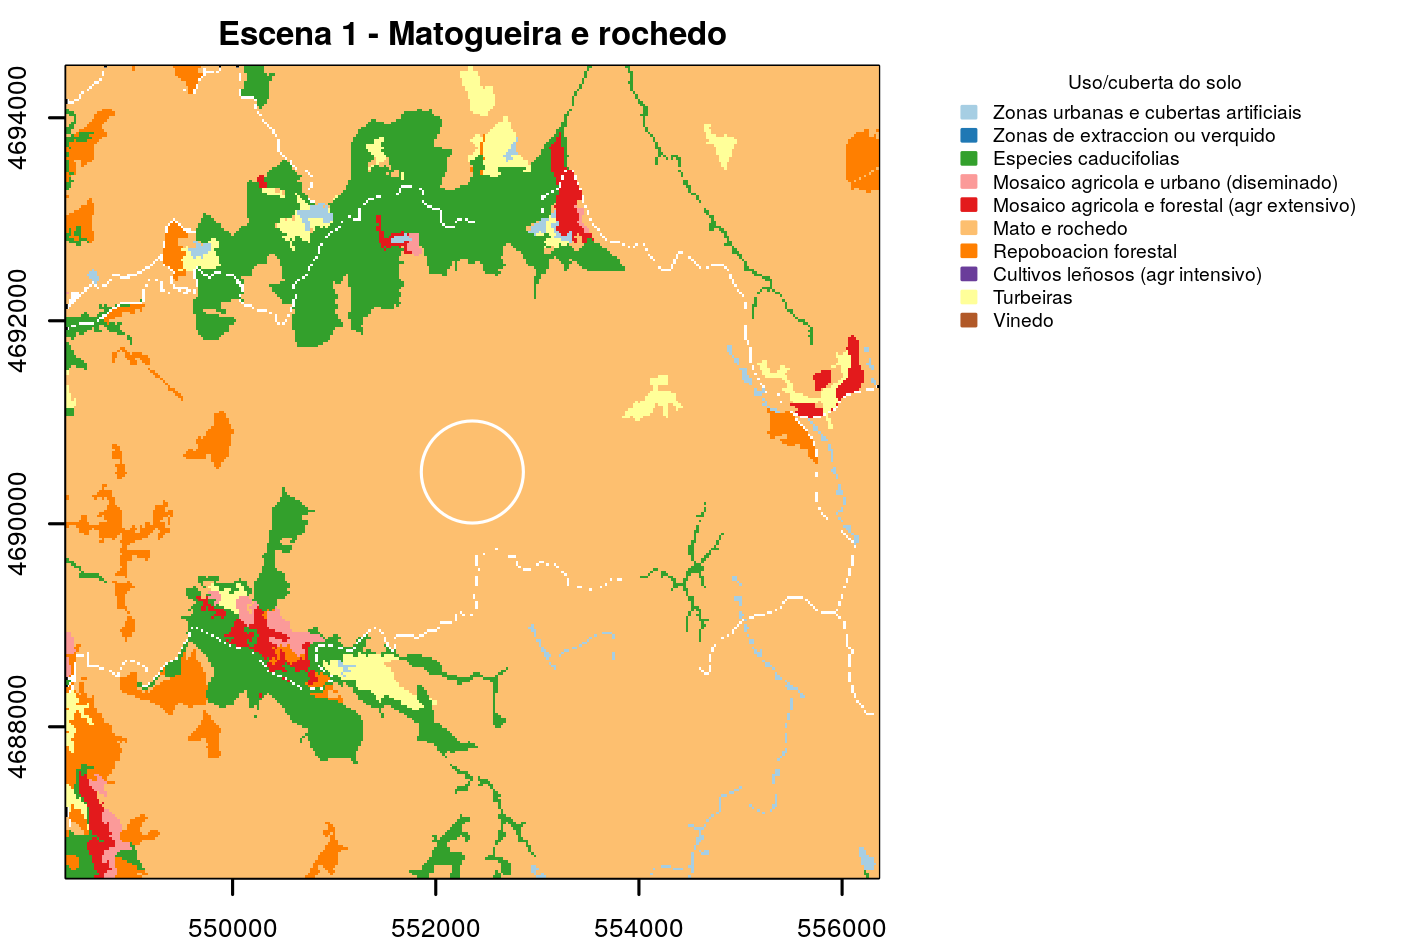
\includegraphics[width=\textwidth]{Escena_1}\\
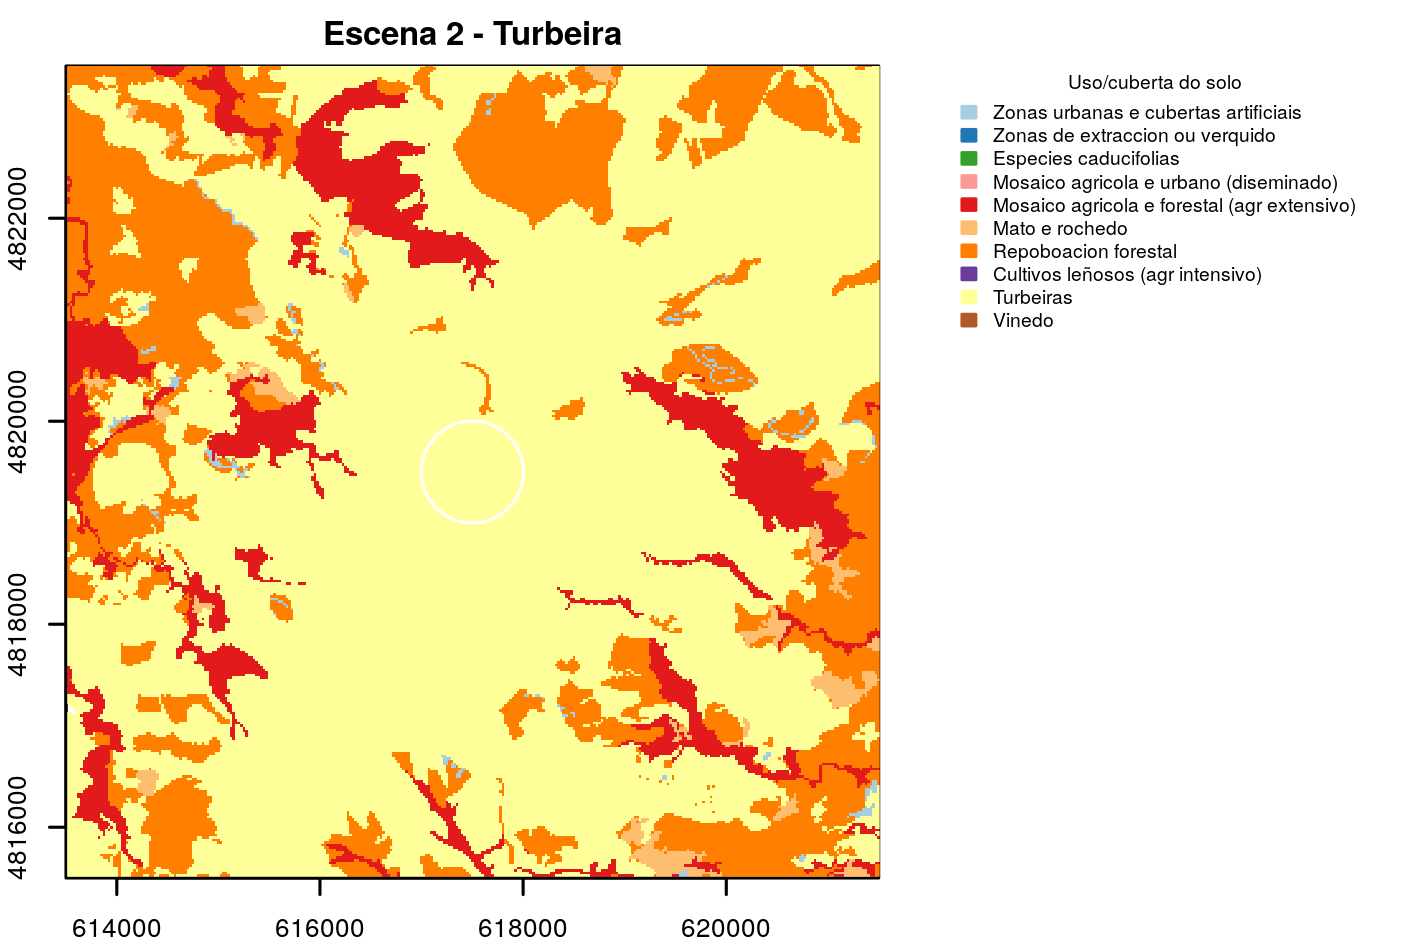
\includegraphics[width=\textwidth]{Escena_2}
\end{figure}

\begin{figure}
\caption{Escenas de entrenamento definidas para áreas de bosque e repoboación forestal}\label{fig:escenas2}
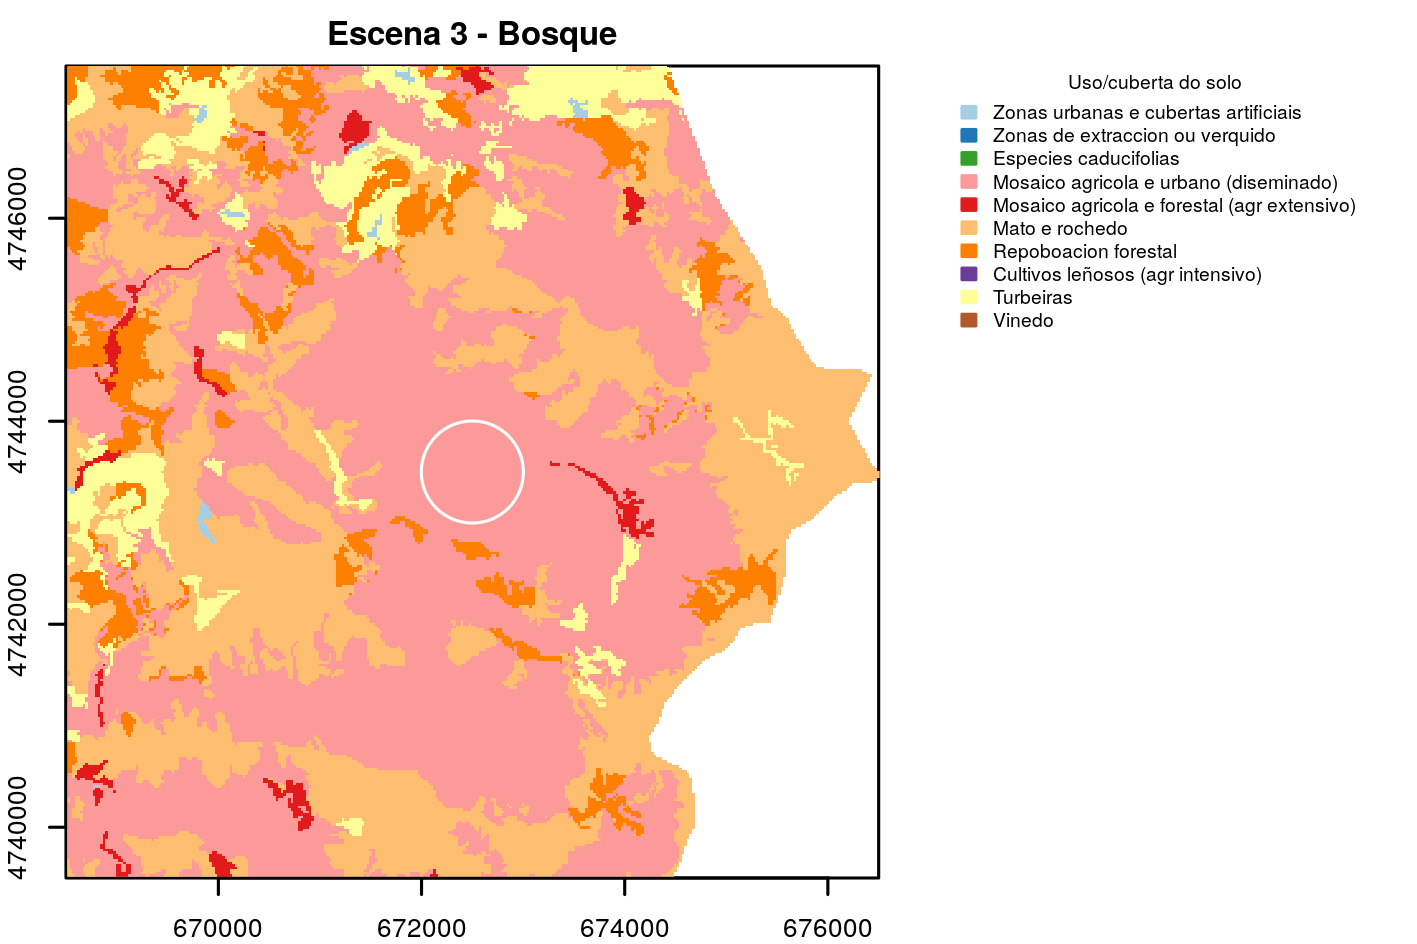
\includegraphics[width=\textwidth]{Escena_3}\\
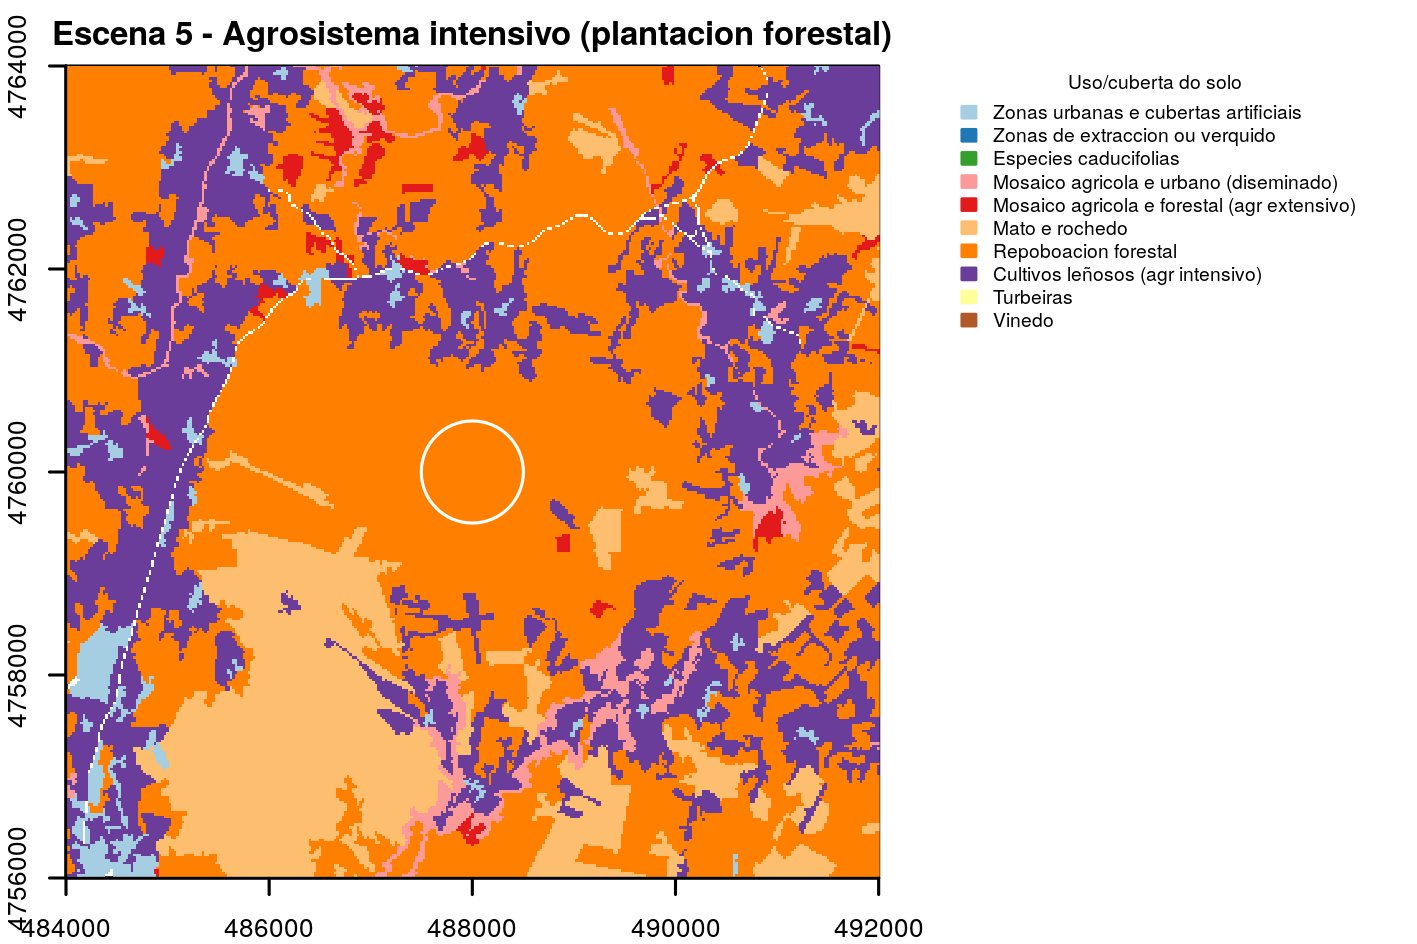
\includegraphics[width=\textwidth]{Escena_5}
\end{figure}

\begin{figure}
\caption{Escena de entrenamento definidas para áreas de uso agrogandeiro intensivo}\label{fig:escenas3}
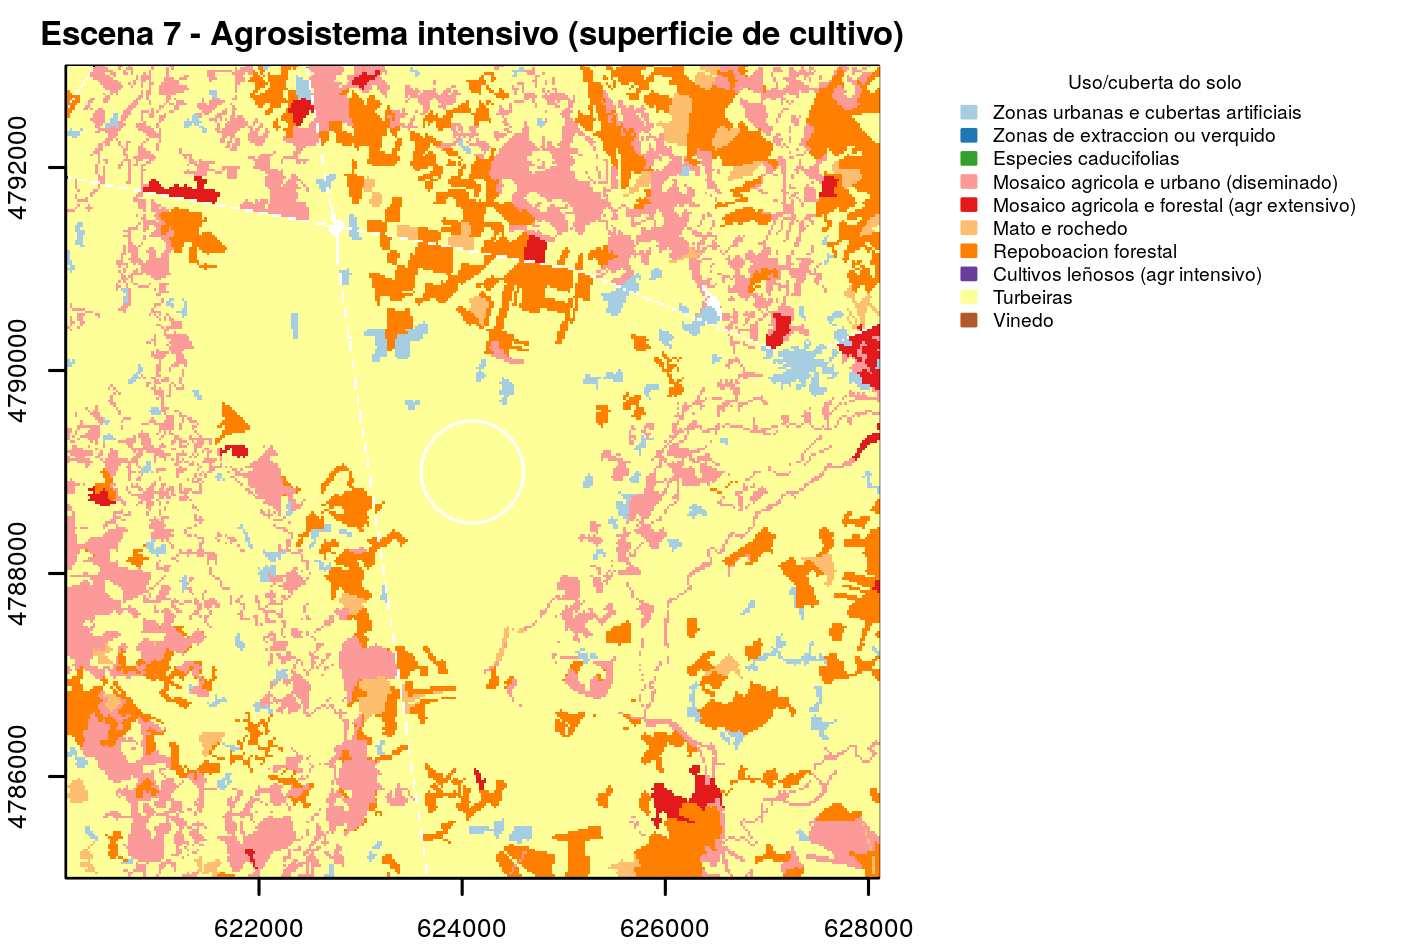
\includegraphics[width=\textwidth]{Escena_7}
\end{figure}

\begin{figure}
\caption{Escenas de entrenamento definidas para áreas de uso agrogandeiro extensivo}\label{fig:escenas4}
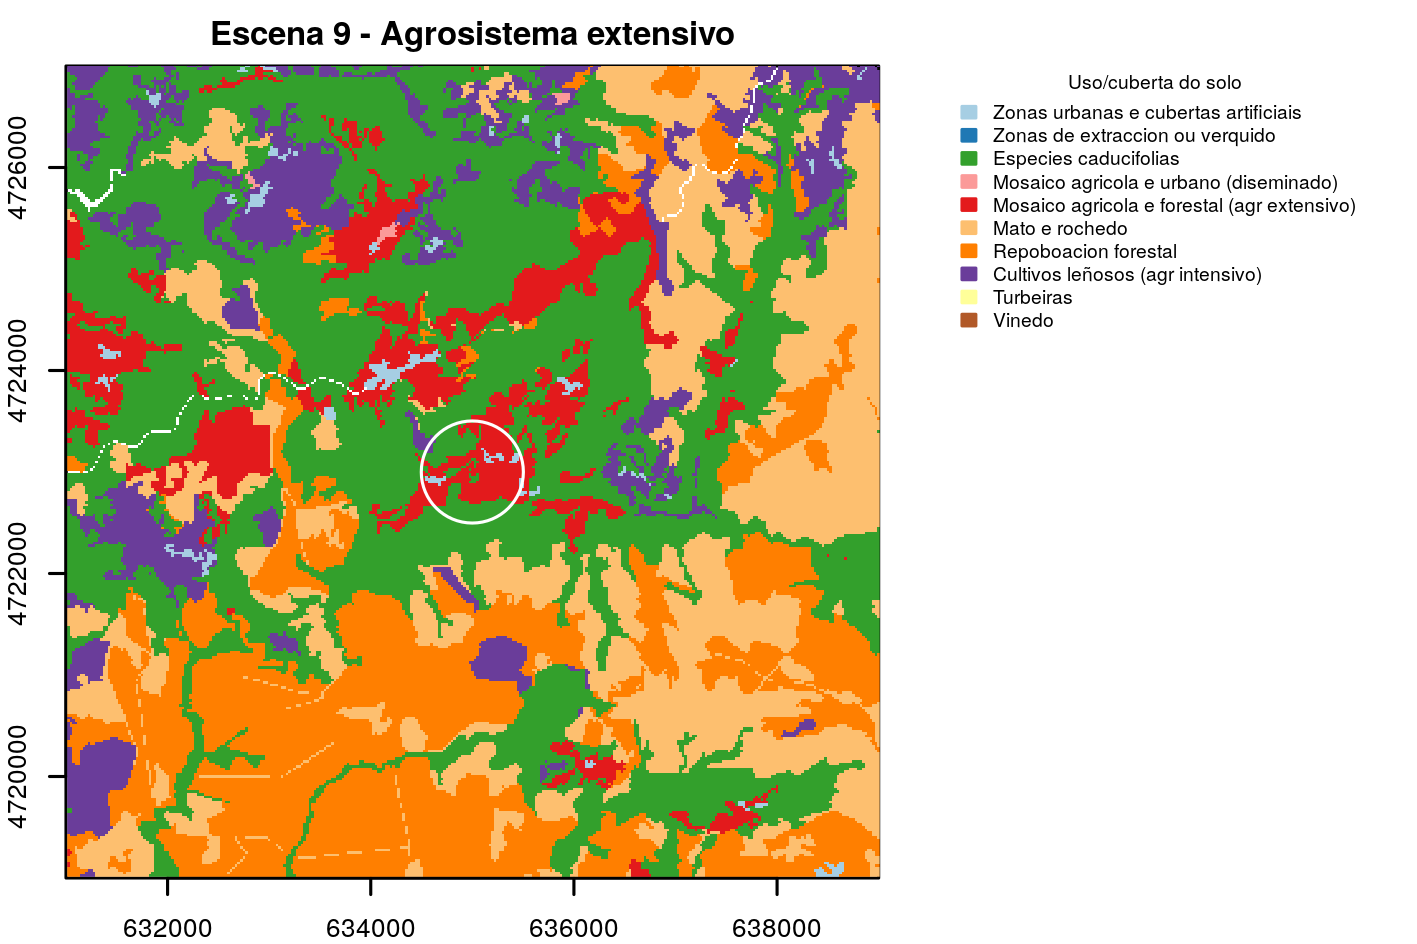
\includegraphics[width=\textwidth]{Escena_9}\\
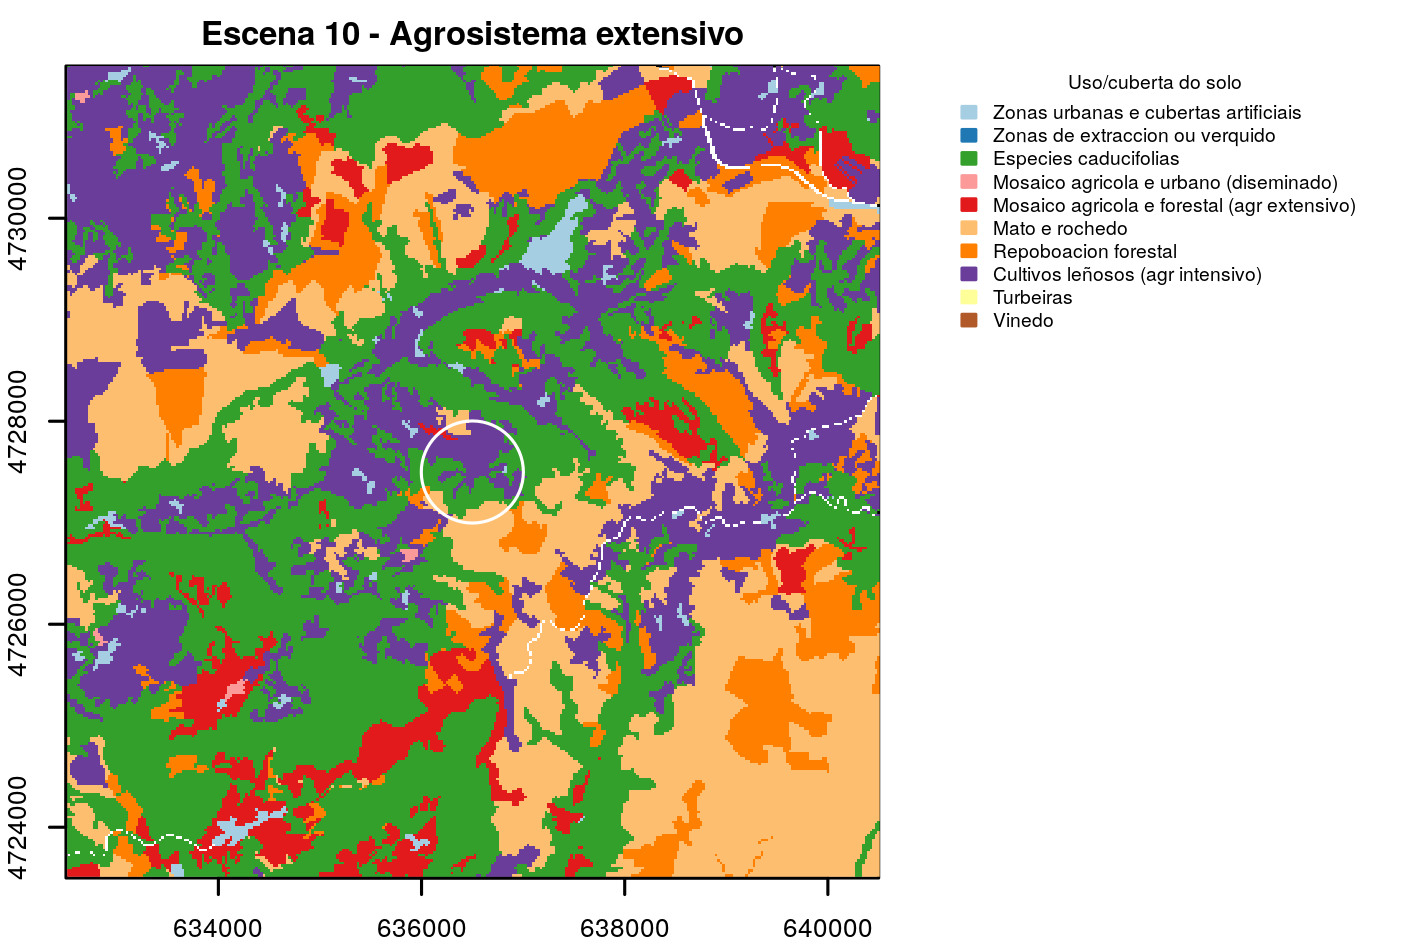
\includegraphics[width=\textwidth]{Escena_10}
\end{figure}

\begin{figure}
\caption{Escenas de entrenamento definidas para áreas de rururbano diseminado}\label{fig:escenas5}
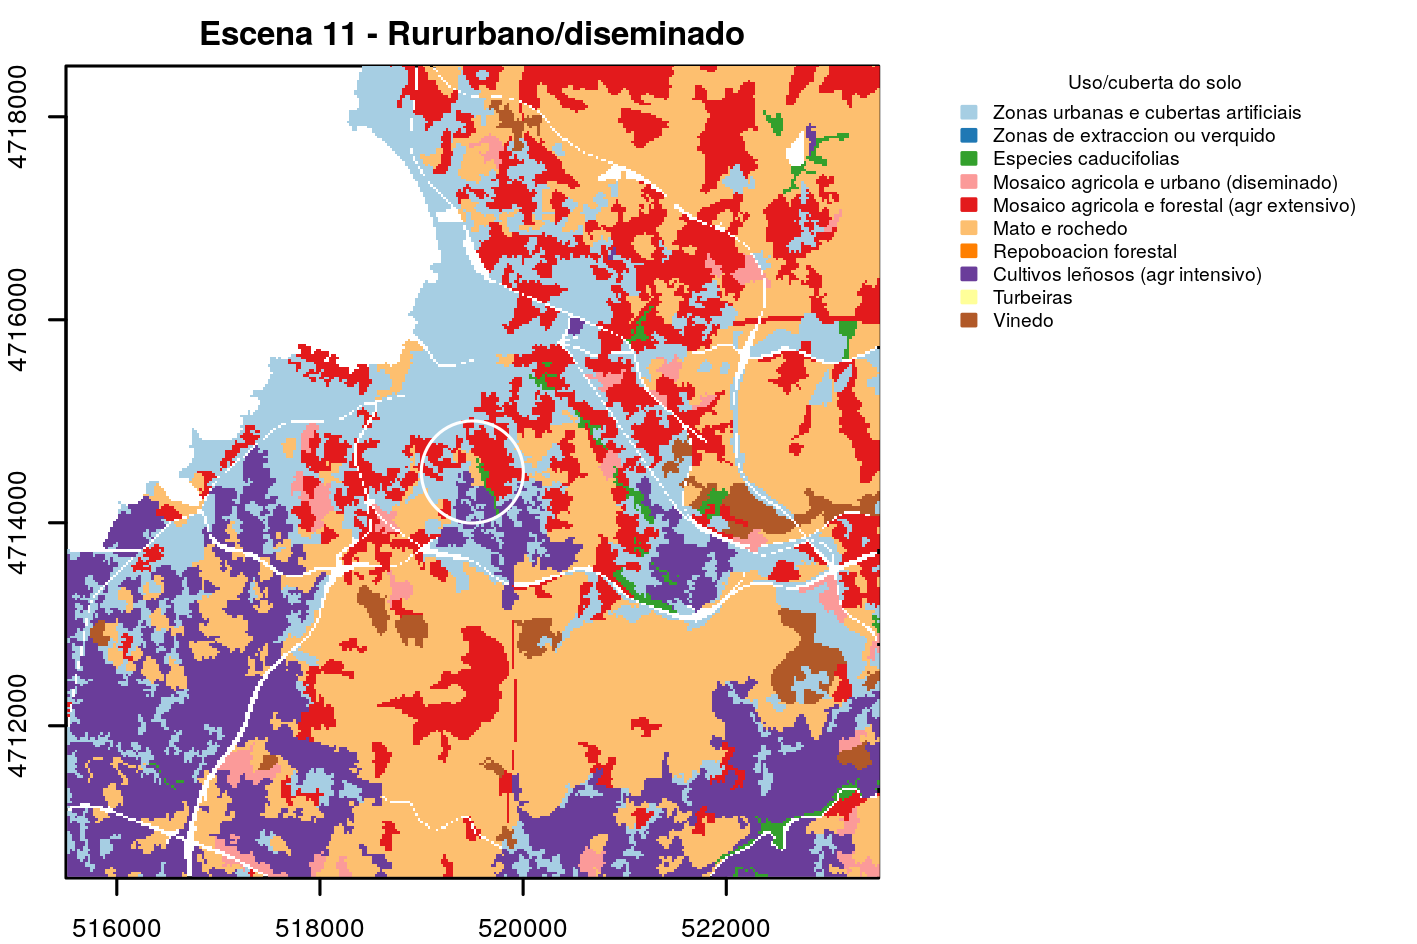
\includegraphics[width=\textwidth]{Escena_11}\\
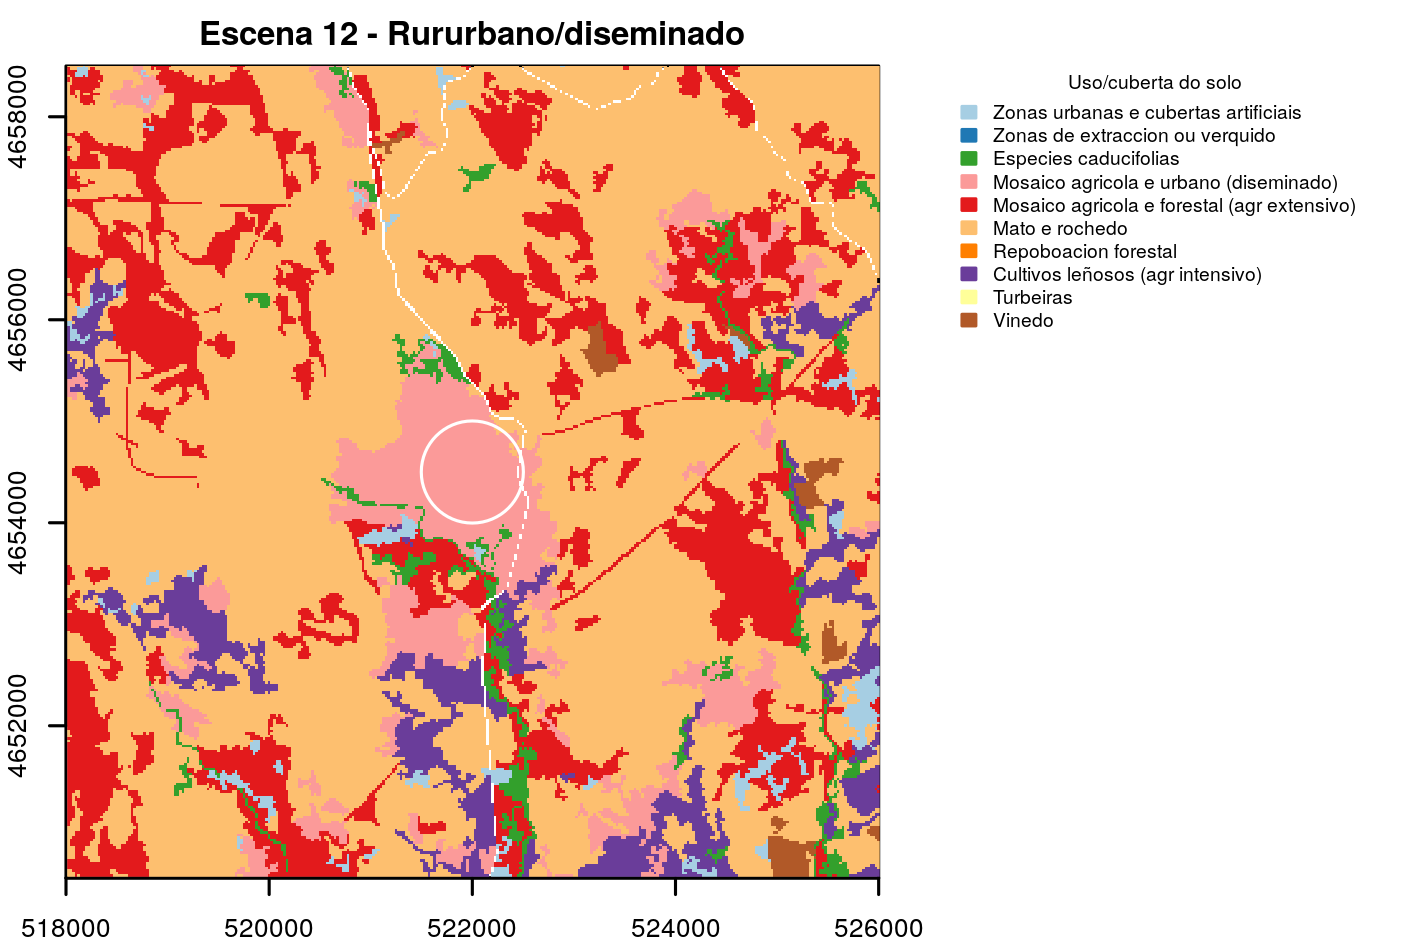
\includegraphics[width=\textwidth]{Escena_12}
\end{figure}

\begin{figure}
\caption{Escenas de entrenamento definidas para áreas urbanas e de uso extractivo}\label{fig:escenas6}
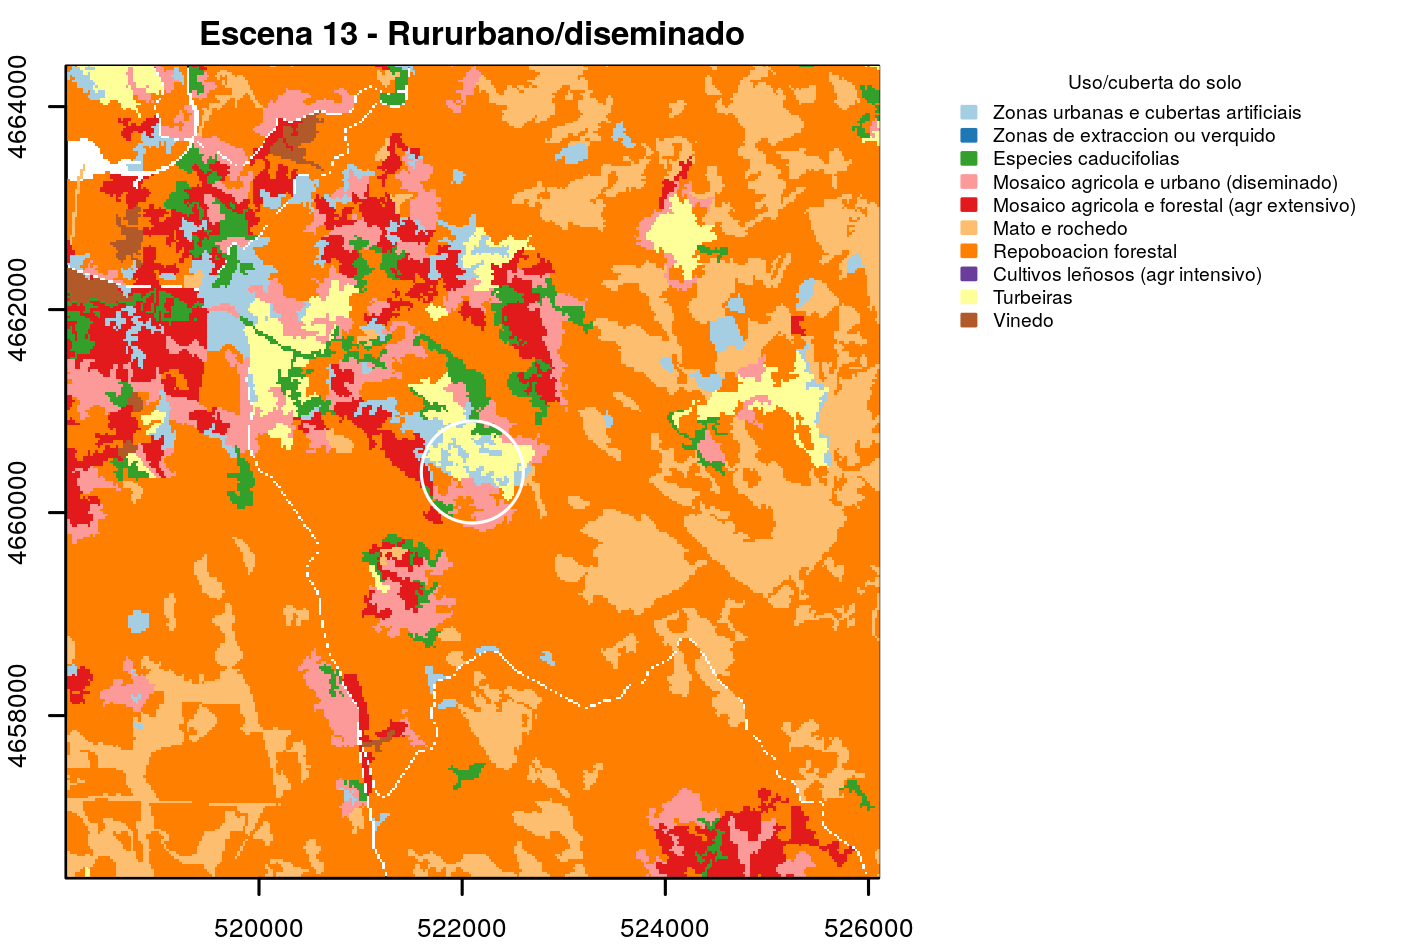
\includegraphics[width=\textwidth]{Escena_13}\\
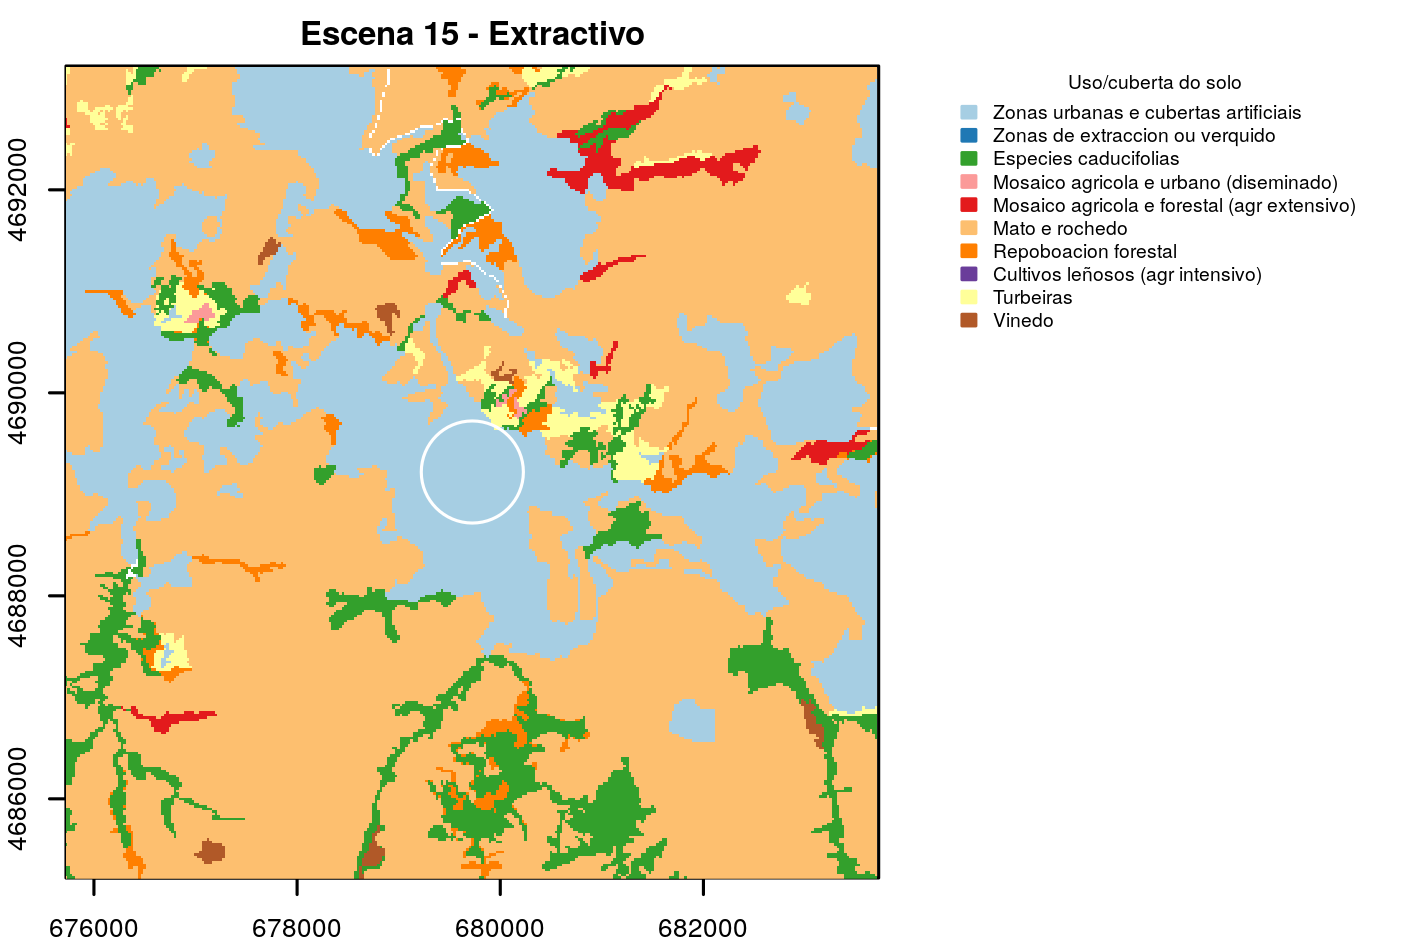
\includegraphics[width=\textwidth]{Escena_15}
\end{figure}

\begin{figure}
\caption{Escenas de entrenamento definidas para áreas de mosaico agroforestal}\label{fig:escenas7}
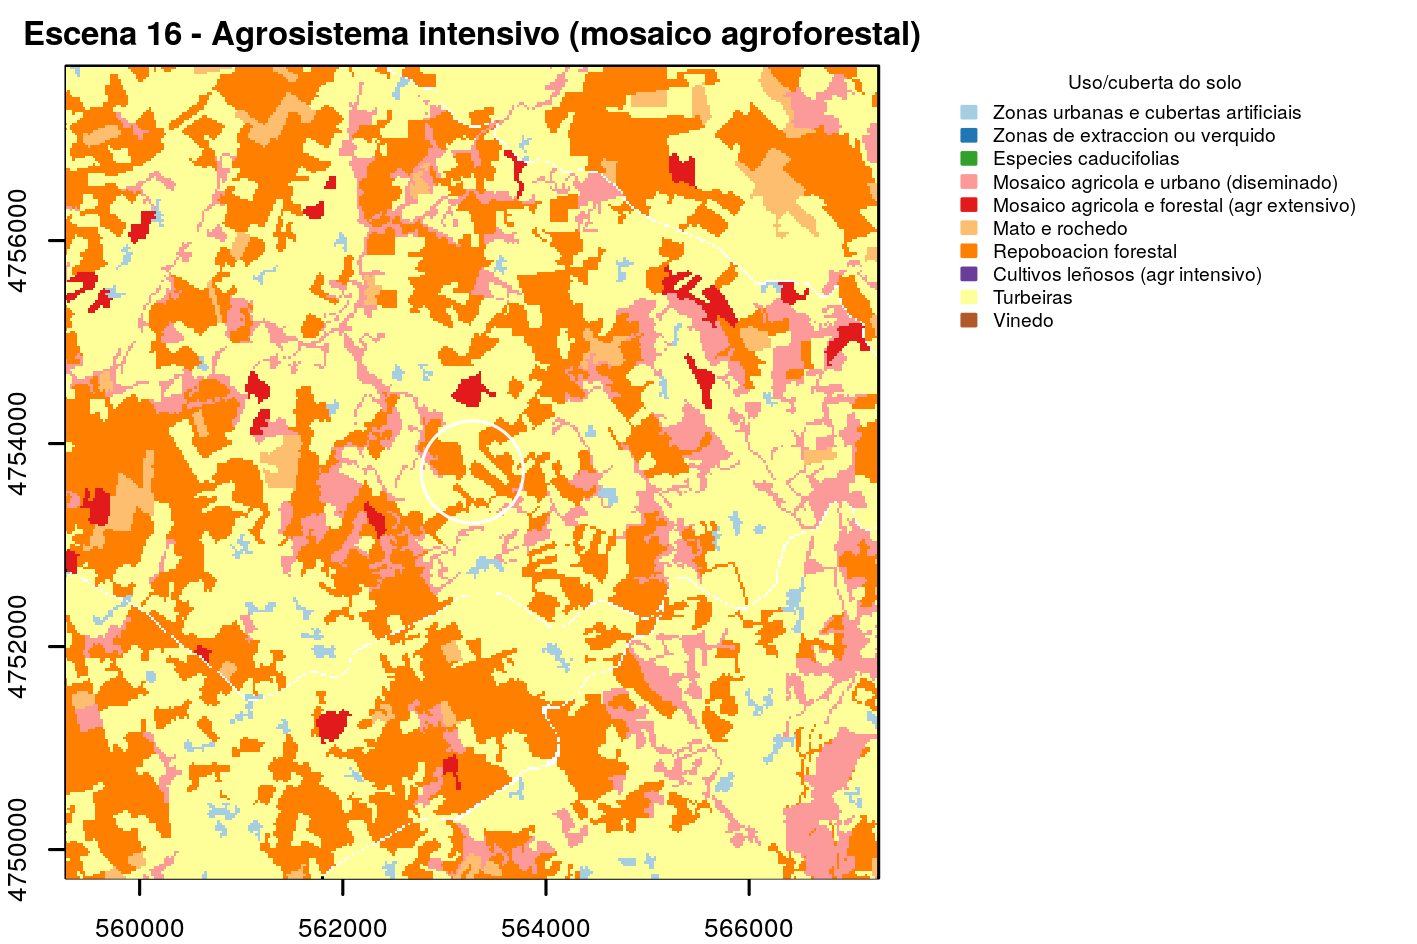
\includegraphics[width=\textwidth]{Escena_16}\\
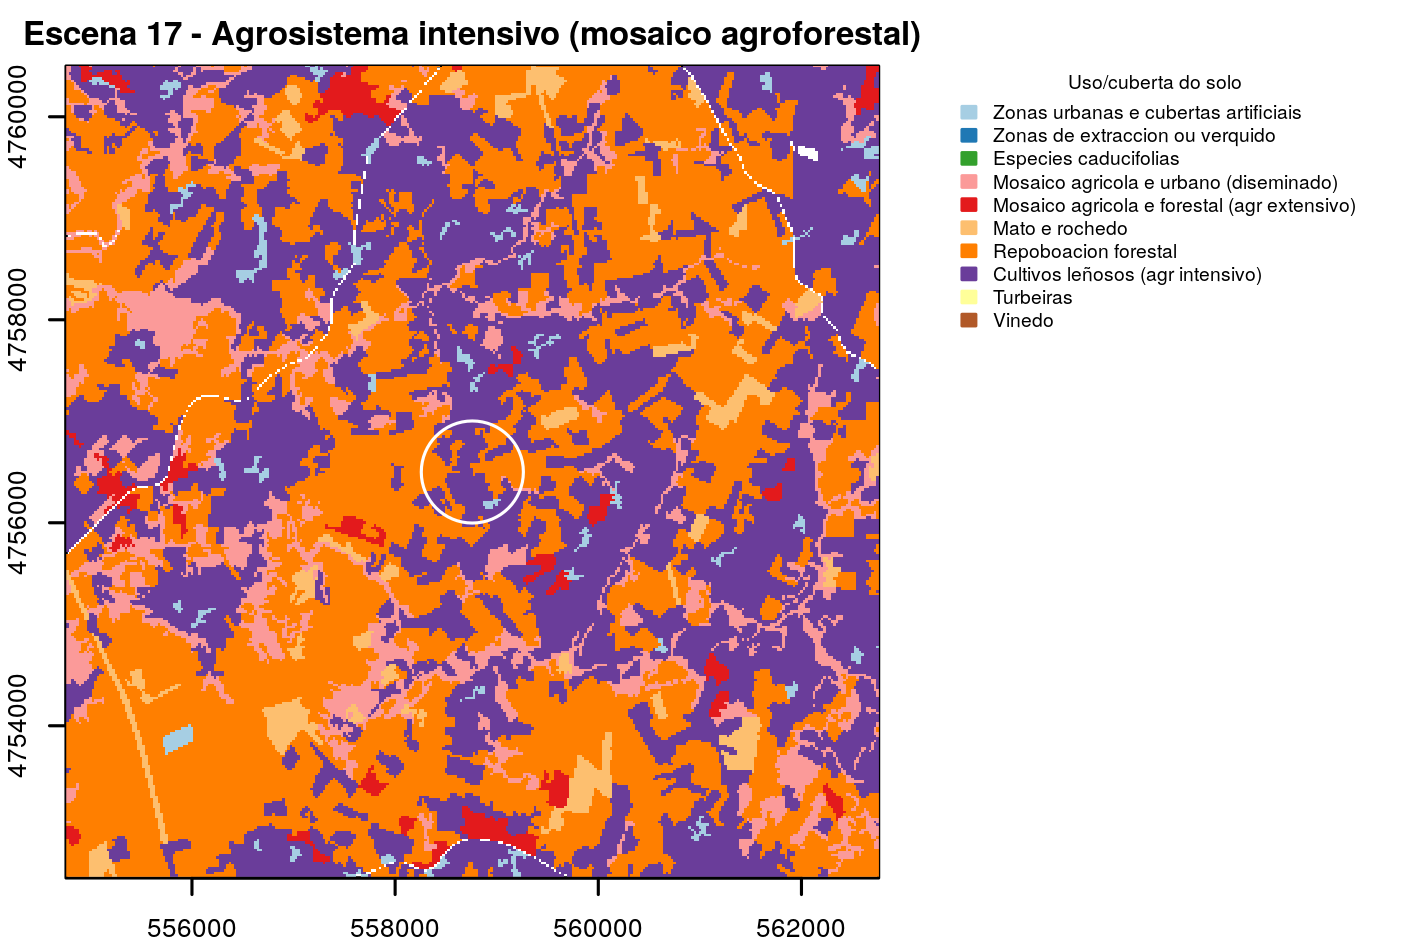
\includegraphics[width=\textwidth]{Escena_17}
\end{figure}

\begin{figure}
\caption{Escenas de entrenamento definidas para áreas de viñedo}\label{fig:escenas8}
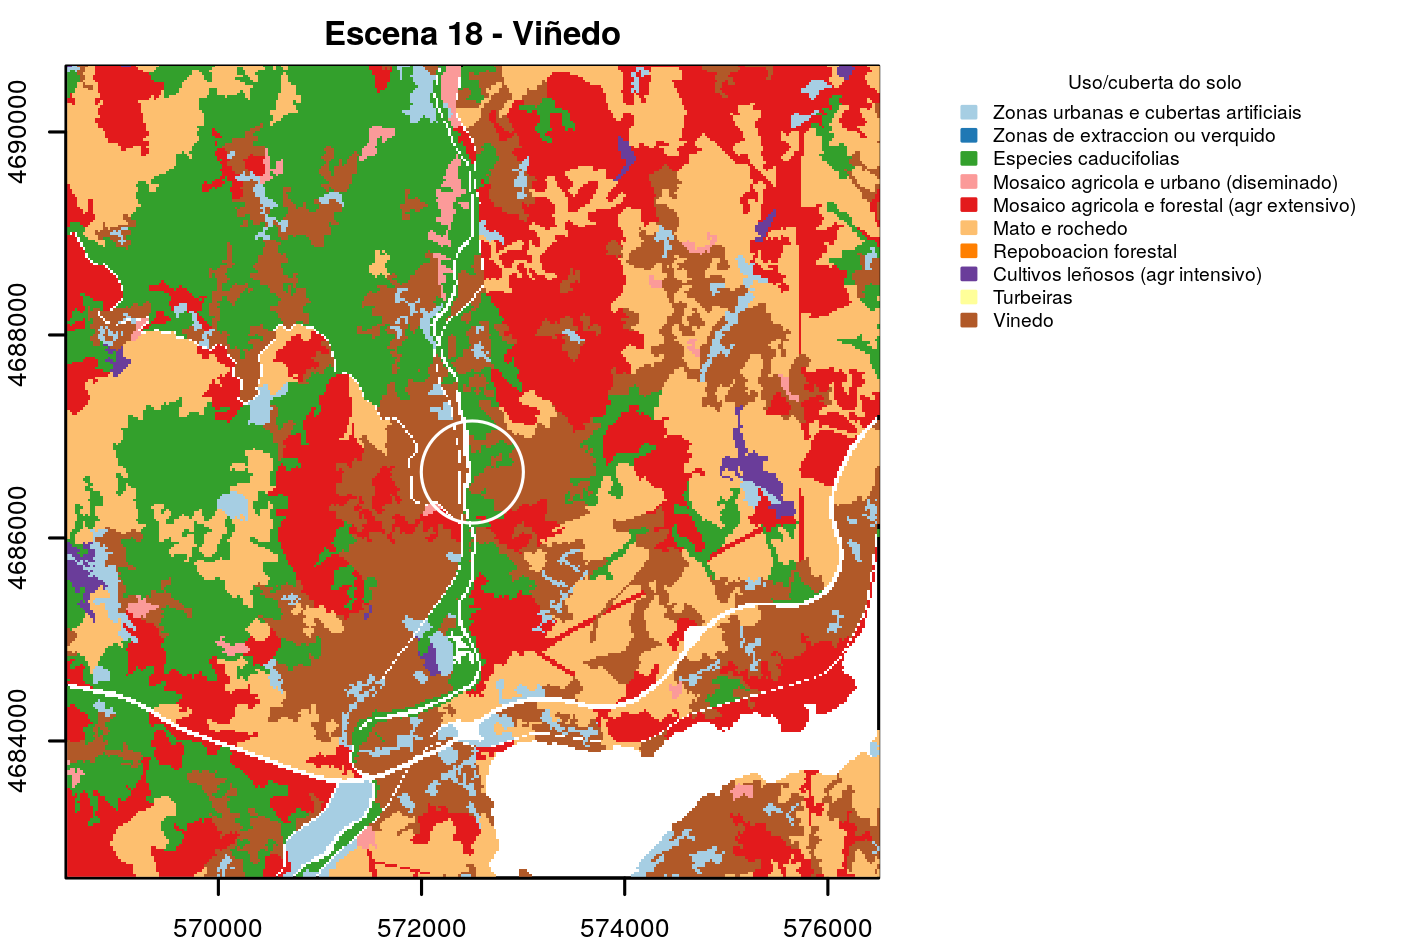
\includegraphics[width=\textwidth]{Escena_18}\\
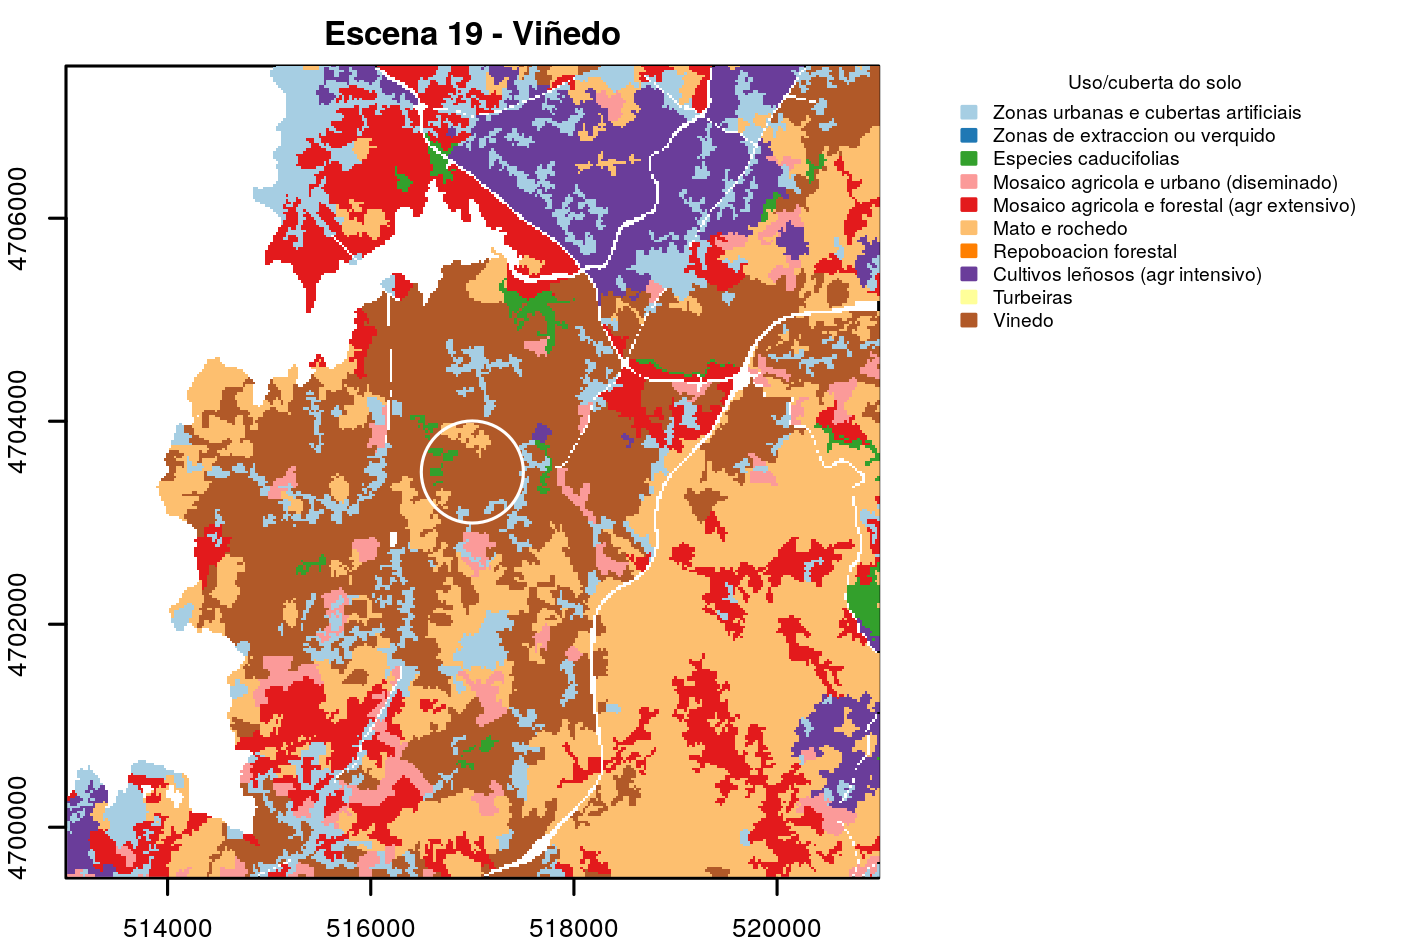
\includegraphics[width=\textwidth]{Escena_19}
\end{figure}

\clearpage


\subsection{Información climática}

A fonte orixinal considera sete clases de termotipos: termotemperado superior, mesotemperado inferior, mesotemperado
superior, supratemperado inferior, supratemperado superior, orotemperado (inferior e superior) e criorotemperado, mesomediterráneo superior. Para facilitar a interpretación do resultado final, neste traballo agrupamos nunha única clase as categorías orixinais de supratemperado inferior, supratemperado superior, orotemperado (inferior e superior) e criorotemperado.

\subsection{Combinación das clases}

Os mapas de clases de formas do terreo e de clases de uso do solo combináronse inicialmente para obter un mapa provisional. Deste mapa, e para mellorar a súa utilidade posterior na xestión, elimináronse as manchas de área menor de 10~ha de superficie. A cada unha das manchas resultantes asignouse unha clase climática (termotipo) mediante unha operación zonal de maioría: é dicir, cada mancha recibiu como atributo o piso termoclimático que ocupaba unha maior parte da súa superficie. Este procedemento permitiu evitar que a información climática, cun nivel de detalle espacial inferior ás dúas outras clases e cunha variabilidade espacial difícil de capturar a esta escala, dividise demasiado as unidades finais. Finalmente, o mapa foi vectorizado de xeito automático.

% No script 4 agora xa se fai o recorte antes da simplificación das áreas de menos de 10ha


\section{Resultados}

Cada tipo de paisaxe contemplado no mapa vén definido, polo tanto, pola combinación das clases dos tres mapas orixinais (excepto para as manchas de cascos históricos, láminas de auga, e praias, que só contan con información de cuberta). En total, a versión 0.6 elaborada de acordo ao descrito neste documento inclúe 20~753 unidades de paisaxe  pertencentes a 185 tipos de paisaxe diferentes, resultantes da combinación das 5 clases de grandes áreas de relevo, 12+3 clases de cuberta do solo, e 5 clases de termotipos (o que resultaría teoricamente en $5\times12\times5 + 3 = 303$ clases teoricamente posibles, das cales non todas aparecen na realidade). A área media das unidades é de 144~ha e a mediana de 21~ha.





\bibliographystyle{galego}
\bibliography{./References/LandscapeMapping}

%\newpage
%\section*{Resumo de tipos de paisaxe por Grandes Áreas Paisaxísticas}

%\begin{landscape}
% \begin{small}
%  % latex table generated in R 3.1.1 by xtable 1.7-4 package
% Fri Oct  2 19:36:23 2015
\begin{table}[p]
\centering
\caption{Grandes Áreas paisaxísticas e código asignado} 
\label{xtaboa0}
\begin{tabular}{rr}
  \hline
 & Código \\ 
  \hline
Golfo Ártabro &   1 \\ 
  A Mariña - Baixo Eo &   2 \\ 
  Costa Sur - Baixo Miño &   3 \\ 
  Ribeiras Encaixadas do Miño e do Sil &   4 \\ 
  Serras Orientais &   5 \\ 
  Chairas e Fosas Luguesas &   6 \\ 
  Galicia Central &   7 \\ 
  Chairas, Fosas e Serras Ourensás &   8 \\ 
  Serras Surorientais &   9 \\ 
  Galicia Setentrional &  10 \\ 
  Chairas e Fosas Occidentais &  11 \\ 
  Rías Baixas &  12 \\ 
   \hline
\end{tabular}
\end{table}
% latex table generated in R 3.1.1 by xtable 1.7-4 package
% Fri Oct  2 19:36:23 2015
\begin{table}[p]
\centering
\caption{Grandes unidades morfolóxicas por Grandes Áreas paisaxísticas (datos en km²)} 
\label{xtaboa1}
\begin{tabular}{rrrrrrrrrrrrr}
  \hline
 & 1 & 2 & 3 & 4 & 5 & 6 & 7 & 8 & 9 & 10 & 11 & 12 \\ 
  \hline
Canons & 36.00 & 0.00 & 0.00 & 318.00 & 41.00 & 6.00 & 0.00 & 0.00 & 82.00 & 0.00 & 0.00 & 0.00 \\ 
  Chairas e vales interiores & 0.00 & 1.00 & 171.00 & 1316.00 & 75.00 & 3217.00 & 231.00 & 1137.00 & 3.00 & 0.00 & 0.00 & 0.00 \\ 
  Litoral Cantabro-Atlantico & 535.00 & 348.00 & 261.00 & 0.00 & 0.00 & 0.00 & 0.00 & 0.00 & 0.00 & 365.00 & 533.00 & 1022.00 \\ 
  Serras & 139.00 & 152.00 & 310.00 & 837.00 & 1794.00 & 1308.00 & 1308.00 & 1705.00 & 2116.00 & 635.00 & 0.00 & 459.00 \\ 
  Vales sublitorais & 577.00 & 424.00 & 392.00 & 1.00 & 584.00 & 28.00 & 3548.00 & 0.00 & 1.00 & 628.00 & 1543.00 & 1219.00 \\ 
   \hline
\end{tabular}
\end{table}
% latex table generated in R 3.1.1 by xtable 1.7-4 package
% Fri Oct  2 19:36:23 2015
\begin{table}[p]
\centering
\caption{Grandes unidades morfolóxicas por Grandes Áreas paisaxísticas (datos en porcentaxe)} 
\label{xtaboa1p}
\begin{tabular}{rrrrrrrrrrrrr}
  \hline
 & 1 & 2 & 3 & 4 & 5 & 6 & 7 & 8 & 9 & 10 & 11 & 12 \\ 
  \hline
Canons & 2.80 & 0.00 & 0.00 & 12.90 & 1.60 & 0.10 & 0.00 & 0.00 & 3.70 & 0.00 & 0.00 & 0.00 \\ 
  Chairas e vales interiores & 0.00 & 0.10 & 14.50 & 53.20 & 3.00 & 70.60 & 4.50 & 40.00 & 0.10 & 0.00 & 0.00 & 0.00 \\ 
  Litoral Cantabro-Atlantico & 41.50 & 37.60 & 22.10 & 0.00 & 0.00 & 0.00 & 0.00 & 0.00 & 0.00 & 22.40 & 25.70 & 37.90 \\ 
  Serras & 10.80 & 16.40 & 26.20 & 33.90 & 71.90 & 28.70 & 25.40 & 60.00 & 96.10 & 39.00 & 0.00 & 17.00 \\ 
  Vales sublitorais & 44.70 & 45.80 & 33.10 & 0.00 & 23.40 & 0.60 & 68.90 & 0.00 & 0.00 & 38.60 & 74.30 & 45.10 \\ 
   \hline
\end{tabular}
\end{table}
% latex table generated in R 3.1.1 by xtable 1.7-4 package
% Fri Oct  2 19:36:23 2015
\begin{table}[p]
\centering
\caption{Clases de cuberta por Grandes Áreas paisaxísticas (datos en km²)} 
\label{xtaboa2}
\begin{tabular}{rrrrrrrrrrrrr}
  \hline
 & 1 & 2 & 3 & 4 & 5 & 6 & 7 & 8 & 9 & 10 & 11 & 12 \\ 
  \hline
Agrosistema extensivo & 68.00 & 25.00 & 62.00 & 622.00 & 963.00 & 1813.00 & 1356.00 & 882.00 & 576.00 & 135.00 & 128.00 & 135.00 \\ 
  Agrosistema intensivo (mosaico agroforestal) & 474.00 & 310.00 & 127.00 & 246.00 & 152.00 & 1253.00 & 1946.00 & 92.00 & 31.00 & 470.00 & 831.00 & 460.00 \\ 
  Agrosistema intensivo (plantacion forestal) & 205.00 & 381.00 & 248.00 & 211.00 & 204.00 & 250.00 & 319.00 & 177.00 & 140.00 & 440.00 & 384.00 & 553.00 \\ 
  Agrosistema intensivo (superficie de cultivo) & 13.00 & 24.00 & 2.00 & 67.00 & 21.00 & 474.00 & 231.00 & 327.00 & 57.00 & 18.00 & 153.00 & 22.00 \\ 
  Bosque & 48.00 & 20.00 & 25.00 & 281.00 & 427.00 & 165.00 & 133.00 & 247.00 & 166.00 & 53.00 & 0.00 & 39.00 \\ 
  Conxunto Historico & 1.00 & 1.00 & 3.00 & 1.00 & 0.00 & 1.00 & 1.00 & 0.00 & 0.00 & 0.00 & 3.00 & 1.00 \\ 
  Extractivo & 0.00 & 0.00 & 6.00 & 2.00 & 4.00 & 0.00 & 7.00 & 3.00 & 22.00 & 12.00 & 1.00 & 0.00 \\ 
  Matogueira e rochedo & 99.00 & 50.00 & 319.00 & 789.00 & 713.00 & 321.00 & 774.00 & 1005.00 & 1195.00 & 213.00 & 388.00 & 703.00 \\ 
  Rururbano (diseminado) & 305.00 & 61.00 & 346.00 & 113.00 & 7.00 & 172.00 & 346.00 & 62.00 & 12.00 & 64.00 & 155.00 & 649.00 \\ 
  Turbeira & 26.00 & 26.00 & 1.00 & 0.00 & 2.00 & 86.00 & 6.00 & 19.00 & 0.00 & 207.00 & 10.00 & 4.00 \\ 
  Urbano & 48.00 & 24.00 & 23.00 & 23.00 & 1.00 & 25.00 & 33.00 & 4.00 & 0.00 & 9.00 & 14.00 & 75.00 \\ 
  Viñedo & 0.00 & 0.00 & 18.00 & 115.00 & 0.00 & 0.00 & 1.00 & 24.00 & 2.00 & 0.00 & 0.00 & 34.00 \\ 
   \hline
\end{tabular}
\end{table}
% latex table generated in R 3.1.1 by xtable 1.7-4 package
% Fri Oct  2 19:36:23 2015
\begin{table}[p]
\centering
\caption{Clases de cuberta por Grandes Áreas paisaxísticas (datos en porcentaxe)} 
\label{xtaboa2p}
\begin{tabular}{rrrrrrrrrrrrr}
  \hline
 & 1 & 2 & 3 & 4 & 5 & 6 & 7 & 8 & 9 & 10 & 11 & 12 \\ 
  \hline
Agrosistema extensivo & 5.30 & 2.70 & 5.20 & 25.20 & 38.60 & 39.80 & 26.30 & 31.00 & 26.20 & 8.30 & 6.20 & 5.00 \\ 
  Agrosistema intensivo (mosaico agroforestal) & 36.70 & 33.50 & 10.70 & 10.00 & 6.10 & 27.50 & 37.80 & 3.20 & 1.40 & 28.90 & 40.00 & 17.00 \\ 
  Agrosistema intensivo (plantacion forestal) & 15.90 & 41.20 & 20.90 & 8.50 & 8.20 & 5.50 & 6.20 & 6.20 & 6.40 & 27.00 & 18.50 & 20.50 \\ 
  Agrosistema intensivo (superficie de cultivo) & 1.00 & 2.60 & 0.20 & 2.70 & 0.80 & 10.40 & 4.50 & 11.50 & 2.60 & 1.10 & 7.40 & 0.80 \\ 
  Bosque & 3.70 & 2.20 & 2.10 & 11.40 & 17.10 & 3.60 & 2.60 & 8.70 & 7.50 & 3.30 & 0.00 & 1.40 \\ 
  Conxunto Historico & 0.10 & 0.10 & 0.30 & 0.00 & 0.00 & 0.00 & 0.00 & 0.00 & 0.00 & 0.00 & 0.10 & 0.00 \\ 
  Extractivo & 0.00 & 0.00 & 0.50 & 0.10 & 0.20 & 0.00 & 0.10 & 0.10 & 1.00 & 0.70 & 0.00 & 0.00 \\ 
  Matogueira e rochedo & 7.70 & 5.40 & 26.90 & 31.90 & 28.60 & 7.00 & 15.00 & 35.30 & 54.30 & 13.10 & 18.70 & 26.00 \\ 
  Rururbano (diseminado) & 23.60 & 6.60 & 29.20 & 4.60 & 0.30 & 3.80 & 6.70 & 2.20 & 0.50 & 3.90 & 7.50 & 24.00 \\ 
  Turbeira & 2.00 & 2.80 & 0.10 & 0.00 & 0.10 & 1.90 & 0.10 & 0.70 & 0.00 & 12.70 & 0.50 & 0.10 \\ 
  Urbano & 3.70 & 2.60 & 1.90 & 0.90 & 0.00 & 0.50 & 0.60 & 0.10 & 0.00 & 0.60 & 0.70 & 2.80 \\ 
  Viñedo & 0.00 & 0.00 & 1.50 & 4.70 & 0.00 & 0.00 & 0.00 & 0.80 & 0.10 & 0.00 & 0.00 & 1.30 \\ 
   \hline
\end{tabular}
\end{table}
% latex table generated in R 3.1.1 by xtable 1.7-4 package
% Fri Oct  2 19:36:23 2015
\begin{table}[p]
\centering
\caption{Termotipos por Grandes Áreas paisaxísticas (datos en km²)} 
\label{xtaboa3}
\begin{tabular}{rrrrrrrrrrrrr}
  \hline
 & 1 & 2 & 3 & 4 & 5 & 6 & 7 & 8 & 9 & 10 & 11 & 12 \\ 
  \hline
Mesomediterráneo & 0.00 & 0.00 & 0.00 & 333.00 & 15.00 & 0.00 & 0.00 & 0.00 & 34.00 & 0.00 & 0.00 & 0.00 \\ 
  Mesotemperado inferior & 417.00 & 474.00 & 204.00 & 1075.00 & 348.00 & 1193.00 & 2932.00 & 1611.00 & 378.00 & 696.00 & 960.00 & 659.00 \\ 
  Mesotemperado superior & 247.00 & 184.00 & 87.00 & 344.00 & 1036.00 & 3148.00 & 1398.00 & 555.00 & 578.00 & 530.00 & 228.00 & 207.00 \\ 
  Supra e orotemperado & 4.00 & 2.00 & 54.00 & 124.00 & 1053.00 & 175.00 & 181.00 & 416.00 & 1202.00 & 107.00 & 0.00 & 71.00 \\ 
  Termotemperado & 610.00 & 262.00 & 822.00 & 595.00 & 34.00 & 43.00 & 642.00 & 243.00 & 0.00 & 285.00 & 867.00 & 1718.00 \\ 
   \hline
\end{tabular}
\end{table}
% latex table generated in R 3.1.1 by xtable 1.7-4 package
% Fri Oct  2 19:36:23 2015
\begin{table}[p]
\centering
\caption{Termotipos por Grandes Áreas paisaxísticas (datos en porcentaxe)} 
\label{xtaboa3p}
\begin{tabular}{rrrrrrrrrrrrr}
  \hline
 & 1 & 2 & 3 & 4 & 5 & 6 & 7 & 8 & 9 & 10 & 11 & 12 \\ 
  \hline
Mesomediterráneo & 0.00 & 0.00 & 0.00 & 13.50 & 0.60 & 0.00 & 0.00 & 0.00 & 1.50 & 0.00 & 0.00 & 0.00 \\ 
  Mesotemperado inferior & 32.30 & 51.20 & 17.20 & 43.50 & 14.00 & 26.20 & 56.90 & 56.60 & 17.20 & 42.80 & 46.20 & 24.40 \\ 
  Mesotemperado superior & 19.10 & 19.90 & 7.40 & 13.90 & 41.50 & 69.10 & 27.10 & 19.50 & 26.30 & 32.60 & 11.00 & 7.70 \\ 
  Supra e orotemperado & 0.30 & 0.20 & 4.60 & 5.00 & 42.20 & 3.80 & 3.50 & 14.60 & 54.60 & 6.60 & 0.00 & 2.60 \\ 
  Termotemperado & 47.30 & 28.30 & 69.50 & 24.10 & 1.40 & 0.90 & 12.50 & 8.50 & 0.00 & 17.50 & 41.80 & 63.60 \\ 
   \hline
\end{tabular}
\end{table}

%  % latex table generated in R 3.2.1 by xtable 1.7-4 package
% Fri Oct  9 10:33:40 2015
\begin{table}[p]
\centering
\caption{Principais tipos de paisaxe,  Golfo Ártabro ( 1 )} 
\label{Tipos 1}
\begin{tabular}{rlrr}
  \hline
 & Tipo & Área (km²) & Porcentaxe \\ 
  \hline
1 & Litoral Cantabro-Atlantico ; Rururbano (diseminado) ; Termotemperado & 249.26 & 19.30 \\ 
  2 & Vales sublitorais ; Agrosistema intensivo (mosaico agroforestal) ; Mesotemperado inferior & 185.89 & 14.40 \\ 
  3 & Litoral Cantabro-Atlantico ; Agrosistema intensivo (mosaico agroforestal) ; Termotemperado & 134.82 & 10.40 \\ 
  4 & Vales sublitorais ; Agrosistema intensivo (plantacion forestal) ; Mesotemperado inferior & 101.37 & 7.90 \\ 
  5 & Vales sublitorais ; Agrosistema intensivo (mosaico agroforestal) ; Mesotemperado superior & 56.41 & 4.40 \\ 
  6 & Vales sublitorais ; Agrosistema intensivo (mosaico agroforestal) ; Termotemperado & 52.42 & 4.10 \\ 
  7 & Litoral Cantabro-Atlantico ; Urbano ; Termotemperado & 40.04 & 3.10 \\ 
  8 & Serras ; Matogueira e rochedo ; Mesotemperado superior & 38.34 & 3.00 \\ 
  9 & Litoral Cantabro-Atlantico ; Agrosistema intensivo (plantacion forestal) ; Termotemperado & 36.56 & 2.80 \\ 
  10 & Vales sublitorais ; Rururbano (diseminado) ; Termotemperado & 27.28 & 2.10 \\ 
  11 & Serras ; Agrosistema extensivo ; Mesotemperado superior & 20.50 & 1.60 \\ 
  12 & Serras ; Agrosistema intensivo (mosaico agroforestal) ; Mesotemperado superior & 21.20 & 1.60 \\ 
  13 & Vales sublitorais ; Agrosistema intensivo (plantacion forestal) ; Termotemperado & 21.27 & 1.60 \\ 
  14 & Serras ; Turbeira ; Mesotemperado superior & 19.36 & 1.50 \\ 
  15 & Vales sublitorais ; Agrosistema intensivo (plantacion forestal) ; Mesotemperado superior & 19.37 & 1.50 \\ 
  16 & Vales sublitorais ; Rururbano (diseminado) ; Mesotemperado inferior & 19.64 & 1.50 \\ 
  17 & Vales sublitorais ; Agrosistema extensivo ; Mesotemperado superior & 17.46 & 1.40 \\ 
  18 & Vales sublitorais ; Matogueira e rochedo ; Mesotemperado inferior & 18.44 & 1.40 \\ 
  19 & Vales sublitorais ; Matogueira e rochedo ; Mesotemperado superior & 15.00 & 1.20 \\ 
  20 & Canons ; Bosque ; Mesotemperado inferior & 13.47 & 1.00 \\ 
  21 & Total & 1108.10 & 85.80 \\ 
   \hline
\end{tabular}
\end{table}
% latex table generated in R 3.2.1 by xtable 1.7-4 package
% Fri Oct  9 10:33:41 2015
\begin{table}[p]
\centering
\caption{Principais tipos de paisaxe,  A Mariña - Baixo Eo ( 2 )} 
\label{Tipos 2}
\begin{tabular}{rlrr}
  \hline
 & Tipo & Área (km²) & Porcentaxe \\ 
  \hline
1 & Vales sublitorais ; Agrosistema intensivo (plantacion forestal) ; Mesotemperado inferior & 129.64 & 14.00 \\ 
  2 & Vales sublitorais ; Agrosistema intensivo (mosaico agroforestal) ; Mesotemperado inferior & 116.09 & 12.60 \\ 
  3 & Litoral Cantabro-Atlantico ; Agrosistema intensivo (plantacion forestal) ; Mesotemperado inferior & 100.27 & 10.80 \\ 
  4 & Litoral Cantabro-Atlantico ; Agrosistema intensivo (mosaico agroforestal) ; Termotemperado & 78.46 & 8.50 \\ 
  5 & Litoral Cantabro-Atlantico ; Agrosistema intensivo (plantacion forestal) ; Termotemperado & 42.72 & 4.60 \\ 
  6 & Litoral Cantabro-Atlantico ; Agrosistema intensivo (mosaico agroforestal) ; Mesotemperado inferior & 39.40 & 4.30 \\ 
  7 & Serras ; Agrosistema intensivo (plantacion forestal) ; Mesotemperado superior & 37.05 & 4.00 \\ 
  8 & Litoral Cantabro-Atlantico ; Rururbano (diseminado) ; Termotemperado & 36.26 & 3.90 \\ 
  9 & Vales sublitorais ; Agrosistema intensivo (mosaico agroforestal) ; Termotemperado & 34.27 & 3.70 \\ 
  10 & Vales sublitorais ; Agrosistema intensivo (plantacion forestal) ; Mesotemperado superior & 29.60 & 3.20 \\ 
  11 & Serras ; Turbeira ; Mesotemperado superior & 21.70 & 2.30 \\ 
  12 & Litoral Cantabro-Atlantico ; Urbano ; Termotemperado & 20.15 & 2.20 \\ 
  13 & Serras ; Agrosistema intensivo (mosaico agroforestal) ; Mesotemperado superior & 20.46 & 2.20 \\ 
  14 & Serras ; Agrosistema intensivo (plantacion forestal) ; Mesotemperado inferior & 20.70 & 2.20 \\ 
  15 & Serras ; Matogueira e rochedo ; Mesotemperado superior & 19.15 & 2.10 \\ 
  16 & Vales sublitorais ; Agrosistema intensivo (plantacion forestal) ; Termotemperado & 19.70 & 2.10 \\ 
  17 & Vales sublitorais ; Agrosistema intensivo (mosaico agroforestal) ; Mesotemperado superior & 15.16 & 1.60 \\ 
  18 & Litoral Cantabro-Atlantico ; Agrosistema intensivo (superficie de cultivo) ; Termotemperado & 13.50 & 1.50 \\ 
  19 & Vales sublitorais ; Matogueira e rochedo ; Mesotemperado inferior & 13.70 & 1.50 \\ 
  20 & Vales sublitorais ; Agrosistema extensivo ; Mesotemperado inferior & 12.22 & 1.30 \\ 
  21 & Vales sublitorais ; Rururbano (diseminado) ; Mesotemperado inferior & 10.73 & 1.20 \\ 
  22 & Total & 830.93 & 89.80 \\ 
   \hline
\end{tabular}
\end{table}
% latex table generated in R 3.2.1 by xtable 1.7-4 package
% Fri Oct  9 10:33:41 2015
\begin{table}[p]
\centering
\caption{Principais tipos de paisaxe,  Costa Sur - Baixo Miño ( 3 )} 
\label{Tipos 3}
\begin{tabular}{rlrr}
  \hline
 & Tipo & Área (km²) & Porcentaxe \\ 
  \hline
1 & Vales sublitorais ; Rururbano (diseminado) ; Termotemperado & 147.82 & 12.50 \\ 
  2 & Litoral Cantabro-Atlantico ; Rururbano (diseminado) ; Termotemperado & 134.98 & 11.40 \\ 
  3 & Vales sublitorais ; Agrosistema intensivo (plantacion forestal) ; Termotemperado & 105.78 & 8.90 \\ 
  4 & Serras ; Matogueira e rochedo ; Mesotemperado superior & 69.70 & 5.90 \\ 
  5 & Serras ; Matogueira e rochedo ; Mesotemperado inferior & 59.84 & 5.10 \\ 
  6 & Serras ; Matogueira e rochedo ; Supra e orotemperado & 50.35 & 4.30 \\ 
  7 & Vales sublitorais ; Matogueira e rochedo ; Termotemperado & 40.45 & 3.40 \\ 
  8 & Litoral Cantabro-Atlantico ; Agrosistema intensivo (mosaico agroforestal) ; Termotemperado & 38.66 & 3.30 \\ 
  9 & Vales sublitorais ; Agrosistema intensivo (mosaico agroforestal) ; Termotemperado & 34.55 & 2.90 \\ 
  10 & Serras ; Agrosistema intensivo (plantacion forestal) ; Termotemperado & 32.95 & 2.80 \\ 
  11 & Chairas e vales interiores ; Matogueira e rochedo ; Mesotemperado inferior & 29.44 & 2.50 \\ 
  12 & Litoral Cantabro-Atlantico ; Agrosistema intensivo (plantacion forestal) ; Termotemperado & 29.68 & 2.50 \\ 
  13 & Chairas e vales interiores ; Rururbano (diseminado) ; Termotemperado & 27.39 & 2.30 \\ 
  14 & Serras ; Agrosistema intensivo (plantacion forestal) ; Mesotemperado inferior & 24.09 & 2.00 \\ 
  15 & Chairas e vales interiores ; Agrosistema intensivo (mosaico agroforestal) ; Termotemperado & 22.70 & 1.90 \\ 
  16 & Chairas e vales interiores ; Agrosistema intensivo (plantacion forestal) ; Termotemperado & 21.85 & 1.80 \\ 
  17 & Serras ; Matogueira e rochedo ; Termotemperado & 20.68 & 1.70 \\ 
  18 & Chairas e vales interiores ; Matogueira e rochedo ; Termotemperado & 17.21 & 1.50 \\ 
  19 & Vales sublitorais ; Agrosistema extensivo ; Termotemperado & 18.00 & 1.50 \\ 
  20 & Litoral Cantabro-Atlantico ; Urbano ; Termotemperado & 17.06 & 1.40 \\ 
  21 & no data ; Rururbano (diseminado) ; Termotemperado & 13.40 & 1.10 \\ 
  22 & Chairas e vales interiores ; Agrosistema intensivo (mosaico agroforestal) ; Mesotemperado inferior & 11.60 & 1.00 \\ 
  23 & Vales sublitorais ; Bosque ; Termotemperado & 12.18 & 1.00 \\ 
  24 & Total & 980.36 & 82.70 \\ 
   \hline
\end{tabular}
\end{table}
% latex table generated in R 3.2.1 by xtable 1.7-4 package
% Fri Oct  9 10:33:41 2015
\begin{table}[p]
\centering
\caption{Principais tipos de paisaxe,  Ribeiras Encaixadas do Miño e do Sil ( 4 )} 
\label{Tipos 4}
\begin{tabular}{rlrr}
  \hline
 & Tipo & Área (km²) & Porcentaxe \\ 
  \hline
1 & Chairas e vales interiores ; Agrosistema extensivo ; Mesotemperado inferior & 226.57 & 9.20 \\ 
  2 & Serras ; Matogueira e rochedo ; Mesotemperado superior & 130.18 & 5.30 \\ 
  3 & Serras ; Matogueira e rochedo ; Mesotemperado inferior & 126.40 & 5.10 \\ 
  4 & Chairas e vales interiores ; Agrosistema intensivo (mosaico agroforestal) ; Mesotemperado inferior & 118.55 & 4.80 \\ 
  5 & Serras ; Agrosistema extensivo ; Mesotemperado inferior & 110.09 & 4.50 \\ 
  6 & Chairas e vales interiores ; Matogueira e rochedo ; Termotemperado & 105.75 & 4.30 \\ 
  7 & Chairas e vales interiores ; Matogueira e rochedo ; Mesotemperado inferior & 103.19 & 4.20 \\ 
  8 & Serras ; Matogueira e rochedo ; Supra e orotemperado & 100.24 & 4.10 \\ 
  9 & Chairas e vales interiores ; Agrosistema extensivo ; Termotemperado & 91.77 & 3.70 \\ 
  10 & Serras ; Agrosistema extensivo ; Mesotemperado superior & 79.50 & 3.20 \\ 
  11 & Chairas e vales interiores ; Matogueira e rochedo ; Mesomediterráneo & 74.02 & 3.00 \\ 
  12 & Chairas e vales interiores ; Rururbano (diseminado) ; Termotemperado & 64.13 & 2.60 \\ 
  13 & Chairas e vales interiores ; Agrosistema intensivo (plantacion forestal) ; Termotemperado & 60.42 & 2.40 \\ 
  14 & Chairas e vales interiores ; Bosque ; Termotemperado & 58.81 & 2.40 \\ 
  15 & Chairas e vales interiores ; Bosque ; Mesotemperado inferior & 58.08 & 2.30 \\ 
  16 & Chairas e vales interiores ; Viñedo ; Termotemperado & 54.56 & 2.20 \\ 
  17 & Canons ; Bosque ; Mesotemperado inferior & 47.00 & 1.90 \\ 
  18 & Canons ; Matogueira e rochedo ; Mesomediterráneo & 43.68 & 1.80 \\ 
  19 & Serras ; Matogueira e rochedo ; Mesomediterráneo & 45.10 & 1.80 \\ 
  20 & Chairas e vales interiores ; Agrosistema intensivo (mosaico agroforestal) ; Termotemperado & 38.34 & 1.60 \\ 
  21 & Chairas e vales interiores ; Agrosistema intensivo (plantacion forestal) ; Mesotemperado inferior & 38.94 & 1.60 \\ 
  22 & Serras ; Agrosistema intensivo (mosaico agroforestal) ; Mesotemperado superior & 38.27 & 1.50 \\ 
  23 & Serras ; Bosque ; Mesotemperado inferior & 36.08 & 1.50 \\ 
  24 & Canons ; Bosque ; Termotemperado & 34.73 & 1.40 \\ 
  25 & Canons ; Matogueira e rochedo ; Mesotemperado inferior & 32.00 & 1.30 \\ 
  26 & Chairas e vales interiores ; Viñedo ; Mesomediterráneo & 33.13 & 1.30 \\ 
  27 & Canons ; Agrosistema extensivo ; Mesotemperado inferior & 29.29 & 1.20 \\ 
  28 & Chairas e vales interiores ; Agrosistema extensivo ; Mesomediterráneo & 30.61 & 1.20 \\ 
  29 & Chairas e vales interiores ; Rururbano (diseminado) ; Mesotemperado inferior & 30.34 & 1.20 \\ 
  30 & Serras ; Agrosistema intensivo (mosaico agroforestal) ; Mesotemperado inferior & 28.86 & 1.20 \\ 
  31 & Chairas e vales interiores ; Agrosistema intensivo (superficie de cultivo) ; Mesotemperado inferior & 23.93 & 1.00 \\ 
  32 & Serras ; Agrosistema intensivo (superficie de cultivo) ; Mesotemperado superior & 24.71 & 1.00 \\ 
  33 & Total & 2117.27 & 85.80 \\ 
   \hline
\end{tabular}
\end{table}
% latex table generated in R 3.2.1 by xtable 1.7-4 package
% Fri Oct  9 10:33:41 2015
\begin{table}[p]
\centering
\caption{Principais tipos de paisaxe,  Serras Orientais ( 5 )} 
\label{Tipos 5}
\begin{tabular}{rlrr}
  \hline
 & Tipo & Área (km²) & Porcentaxe \\ 
  \hline
1 & Serras ; Agrosistema extensivo ; Supra e orotemperado & 378.25 & 15.20 \\ 
  2 & Serras ; Matogueira e rochedo ; Supra e orotemperado & 369.67 & 14.80 \\ 
  3 & Serras ; Agrosistema extensivo ; Mesotemperado superior & 295.32 & 11.80 \\ 
  4 & Serras ; Matogueira e rochedo ; Mesotemperado superior & 172.18 & 6.90 \\ 
  5 & Vales sublitorais ; Agrosistema extensivo ; Mesotemperado superior & 141.35 & 5.70 \\ 
  6 & Serras ; Bosque ; Supra e orotemperado & 128.80 & 5.20 \\ 
  7 & Vales sublitorais ; Agrosistema extensivo ; Mesotemperado inferior & 97.14 & 3.90 \\ 
  8 & Serras ; Bosque ; Mesotemperado superior & 94.25 & 3.80 \\ 
  9 & Vales sublitorais ; Bosque ; Mesotemperado superior & 86.92 & 3.50 \\ 
  10 & Serras ; Agrosistema intensivo (plantacion forestal) ; Supra e orotemperado & 85.44 & 3.40 \\ 
  11 & Vales sublitorais ; Bosque ; Mesotemperado inferior & 70.38 & 2.80 \\ 
  12 & Vales sublitorais ; Matogueira e rochedo ; Mesotemperado superior & 61.69 & 2.50 \\ 
  13 & Serras ; Agrosistema intensivo (mosaico agroforestal) ; Supra e orotemperado & 60.90 & 2.40 \\ 
  14 & Serras ; Agrosistema intensivo (plantacion forestal) ; Mesotemperado superior & 58.11 & 2.30 \\ 
  15 & Serras ; Agrosistema intensivo (mosaico agroforestal) ; Mesotemperado superior & 48.86 & 2.00 \\ 
  16 & Vales sublitorais ; Matogueira e rochedo ; Mesotemperado inferior & 39.81 & 1.60 \\ 
  17 & Serras ; Matogueira e rochedo ; Mesotemperado inferior & 27.49 & 1.10 \\ 
  18 & Total & 2216.56 & 88.90 \\ 
   \hline
\end{tabular}
\end{table}
% latex table generated in R 3.2.1 by xtable 1.7-4 package
% Fri Oct  9 10:33:41 2015
\begin{table}[p]
\centering
\caption{Principais tipos de paisaxe,  Chairas e Fosas Luguesas ( 6 )} 
\label{Tipos 6}
\begin{tabular}{rlrr}
  \hline
 & Tipo & Área (km²) & Porcentaxe \\ 
  \hline
1 & Chairas e vales interiores ; Agrosistema extensivo ; Mesotemperado superior & 797.87 & 17.50 \\ 
  2 & Chairas e vales interiores ; Agrosistema intensivo (mosaico agroforestal) ; Mesotemperado superior & 664.75 & 14.60 \\ 
  3 & Serras ; Agrosistema extensivo ; Mesotemperado superior & 462.36 & 10.10 \\ 
  4 & Chairas e vales interiores ; Agrosistema extensivo ; Mesotemperado inferior & 436.22 & 9.60 \\ 
  5 & Chairas e vales interiores ; Agrosistema intensivo (mosaico agroforestal) ; Mesotemperado inferior & 295.64 & 6.50 \\ 
  6 & Serras ; Agrosistema intensivo (mosaico agroforestal) ; Mesotemperado superior & 246.83 & 5.40 \\ 
  7 & Chairas e vales interiores ; Agrosistema intensivo (superficie de cultivo) ; Mesotemperado superior & 208.92 & 4.60 \\ 
  8 & Serras ; Agrosistema intensivo (superficie de cultivo) ; Mesotemperado superior & 132.67 & 2.90 \\ 
  9 & Chairas e vales interiores ; Agrosistema intensivo (plantacion forestal) ; Mesotemperado superior & 118.95 & 2.60 \\ 
  10 & Chairas e vales interiores ; Agrosistema intensivo (superficie de cultivo) ; Mesotemperado inferior & 106.27 & 2.30 \\ 
  11 & Chairas e vales interiores ; Matogueira e rochedo ; Mesotemperado inferior & 89.08 & 2.00 \\ 
  12 & Chairas e vales interiores ; Matogueira e rochedo ; Mesotemperado superior & 87.81 & 1.90 \\ 
  13 & Chairas e vales interiores ; Rururbano (diseminado) ; Mesotemperado superior & 88.58 & 1.90 \\ 
  14 & Serras ; Matogueira e rochedo ; Mesotemperado superior & 81.24 & 1.80 \\ 
  15 & Chairas e vales interiores ; Bosque ; Mesotemperado superior & 69.92 & 1.50 \\ 
  16 & Chairas e vales interiores ; Rururbano (diseminado) ; Mesotemperado inferior & 64.35 & 1.40 \\ 
  17 & Chairas e vales interiores ; Bosque ; Mesotemperado inferior & 58.90 & 1.30 \\ 
  18 & Serras ; Agrosistema intensivo (plantacion forestal) ; Mesotemperado superior & 60.75 & 1.30 \\ 
  19 & Serras ; Agrosistema extensivo ; Supra e orotemperado & 49.88 & 1.10 \\ 
  20 & Serras ; Turbeira ; Mesotemperado superior & 51.82 & 1.10 \\ 
  21 & Total & 4172.81 & 91.40 \\ 
   \hline
\end{tabular}
\end{table}
% latex table generated in R 3.2.1 by xtable 1.7-4 package
% Fri Oct  9 10:33:41 2015
\begin{table}[p]
\centering
\caption{Principais tipos de paisaxe,  Galicia Central ( 7 )} 
\label{Tipos 7}
\begin{tabular}{rlrr}
  \hline
 & Tipo & Área (km²) & Porcentaxe \\ 
  \hline
1 & Vales sublitorais ; Agrosistema intensivo (mosaico agroforestal) ; Mesotemperado inferior & 1225.74 & 23.80 \\ 
  2 & Vales sublitorais ; Agrosistema extensivo ; Mesotemperado inferior & 535.39 & 10.40 \\ 
  3 & Serras ; Agrosistema extensivo ; Mesotemperado superior & 363.58 & 7.10 \\ 
  4 & Vales sublitorais ; Agrosistema intensivo (mosaico agroforestal) ; Termotemperado & 298.29 & 5.80 \\ 
  5 & Serras ; Matogueira e rochedo ; Mesotemperado superior & 257.51 & 5.00 \\ 
  6 & Vales sublitorais ; Agrosistema intensivo (mosaico agroforestal) ; Mesotemperado superior & 226.65 & 4.40 \\ 
  7 & Vales sublitorais ; Rururbano (diseminado) ; Mesotemperado inferior & 188.56 & 3.70 \\ 
  8 & Vales sublitorais ; Matogueira e rochedo ; Mesotemperado inferior & 160.57 & 3.10 \\ 
  9 & Vales sublitorais ; Agrosistema extensivo ; Mesotemperado superior & 150.12 & 2.90 \\ 
  10 & Serras ; Agrosistema extensivo ; Mesotemperado inferior & 137.54 & 2.70 \\ 
  11 & Vales sublitorais ; Agrosistema intensivo (plantacion forestal) ; Mesotemperado inferior & 140.19 & 2.70 \\ 
  12 & Vales sublitorais ; Agrosistema intensivo (superficie de cultivo) ; Mesotemperado inferior & 126.21 & 2.40 \\ 
  13 & Serras ; Matogueira e rochedo ; Supra e orotemperado & 113.08 & 2.20 \\ 
  14 & Vales sublitorais ; Rururbano (diseminado) ; Termotemperado & 99.95 & 1.90 \\ 
  15 & Serras ; Agrosistema intensivo (mosaico agroforestal) ; Mesotemperado superior & 82.78 & 1.60 \\ 
  16 & Serras ; Matogueira e rochedo ; Mesotemperado inferior & 83.06 & 1.60 \\ 
  17 & Vales sublitorais ; Agrosistema intensivo (plantacion forestal) ; Termotemperado & 62.40 & 1.20 \\ 
  18 & Vales sublitorais ; Matogueira e rochedo ; Mesotemperado superior & 55.11 & 1.10 \\ 
  19 & Vales sublitorais ; Agrosistema extensivo ; Termotemperado & 49.53 & 1.00 \\ 
  20 & Total & 4356.26 & 84.60 \\ 
   \hline
\end{tabular}
\end{table}
% latex table generated in R 3.2.1 by xtable 1.7-4 package
% Fri Oct  9 10:33:41 2015
\begin{table}[p]
\centering
\caption{Principais tipos de paisaxe,  Chairas, Fosas e Serras Ourensás ( 8 )} 
\label{Tipos 8}
\begin{tabular}{rlrr}
  \hline
 & Tipo & Área (km²) & Porcentaxe \\ 
  \hline
1 & Chairas e vales interiores ; Agrosistema extensivo ; Mesotemperado inferior & 342.76 & 12.00 \\ 
  2 & Serras ; Matogueira e rochedo ; Mesotemperado superior & 284.07 & 10.00 \\ 
  3 & Serras ; Agrosistema extensivo ; Mesotemperado inferior & 256.71 & 9.00 \\ 
  4 & Serras ; Matogueira e rochedo ; Mesotemperado inferior & 255.53 & 9.00 \\ 
  5 & Serras ; Matogueira e rochedo ; Supra e orotemperado & 239.60 & 8.40 \\ 
  6 & Chairas e vales interiores ; Agrosistema intensivo (superficie de cultivo) ; Mesotemperado inferior & 212.46 & 7.50 \\ 
  7 & Serras ; Agrosistema extensivo ; Mesotemperado superior & 140.13 & 4.90 \\ 
  8 & Chairas e vales interiores ; Matogueira e rochedo ; Mesotemperado inferior & 136.15 & 4.80 \\ 
  9 & Serras ; Agrosistema extensivo ; Supra e orotemperado & 87.82 & 3.10 \\ 
  10 & Chairas e vales interiores ; Bosque ; Mesotemperado inferior & 79.78 & 2.80 \\ 
  11 & Serras ; Bosque ; Mesotemperado inferior & 76.28 & 2.70 \\ 
  12 & Chairas e vales interiores ; Matogueira e rochedo ; Termotemperado & 61.48 & 2.20 \\ 
  13 & Serras ; Agrosistema intensivo (plantacion forestal) ; Mesotemperado inferior & 56.85 & 2.00 \\ 
  14 & Chairas e vales interiores ; Agrosistema extensivo ; Termotemperado & 50.49 & 1.80 \\ 
  15 & Chairas e vales interiores ; Agrosistema intensivo (plantacion forestal) ; Mesotemperado inferior & 46.95 & 1.70 \\ 
  16 & Serras ; Agrosistema intensivo (superficie de cultivo) ; Mesotemperado inferior & 46.12 & 1.60 \\ 
  17 & Serras ; Bosque ; Mesotemperado superior & 45.85 & 1.60 \\ 
  18 & Chairas e vales interiores ; Agrosistema intensivo (mosaico agroforestal) ; Mesotemperado inferior & 41.06 & 1.40 \\ 
  19 & Serras ; Agrosistema intensivo (superficie de cultivo) ; Mesotemperado superior & 35.88 & 1.30 \\ 
  20 & Chairas e vales interiores ; Agrosistema intensivo (mosaico agroforestal) ; Termotemperado & 34.03 & 1.20 \\ 
  21 & Chairas e vales interiores ; Rururbano (diseminado) ; Mesotemperado inferior & 34.69 & 1.20 \\ 
  22 & Serras ; Agrosistema intensivo (plantacion forestal) ; Mesotemperado superior & 31.71 & 1.10 \\ 
  23 & Serras ; Bosque ; Supra e orotemperado & 27.73 & 1.00 \\ 
  24 & Total & 2624.13 & 92.30 \\ 
   \hline
\end{tabular}
\end{table}
% latex table generated in R 3.2.1 by xtable 1.7-4 package
% Fri Oct  9 10:33:41 2015
\begin{table}[p]
\centering
\caption{Principais tipos de paisaxe,  Serras Surorientais ( 9 )} 
\label{Tipos 9}
\begin{tabular}{rlrr}
  \hline
 & Tipo & Área (km²) & Porcentaxe \\ 
  \hline
1 & Serras ; Matogueira e rochedo ; Supra e orotemperado & 825.10 & 37.50 \\ 
  2 & Serras ; Agrosistema extensivo ; Mesotemperado superior & 229.18 & 10.40 \\ 
  3 & Serras ; Matogueira e rochedo ; Mesotemperado superior & 218.13 & 9.90 \\ 
  4 & Serras ; Agrosistema extensivo ; Supra e orotemperado & 165.93 & 7.50 \\ 
  5 & Serras ; Agrosistema extensivo ; Mesotemperado inferior & 155.37 & 7.10 \\ 
  6 & Serras ; Agrosistema intensivo (plantacion forestal) ; Supra e orotemperado & 112.84 & 5.10 \\ 
  7 & Serras ; Matogueira e rochedo ; Mesotemperado inferior & 91.96 & 4.20 \\ 
  8 & Serras ; Bosque ; Mesotemperado superior & 56.72 & 2.60 \\ 
  9 & Serras ; Bosque ; Supra e orotemperado & 45.21 & 2.10 \\ 
  10 & Serras ; Bosque ; Mesotemperado inferior & 43.08 & 2.00 \\ 
  11 & Serras ; Agrosistema intensivo (superficie de cultivo) ; Mesotemperado superior & 25.28 & 1.10 \\ 
  12 & Total & 1968.80 & 89.50 \\ 
   \hline
\end{tabular}
\end{table}
% latex table generated in R 3.2.1 by xtable 1.7-4 package
% Fri Oct  9 10:33:41 2015
\begin{table}[p]
\centering
\caption{Principais tipos de paisaxe,  Galicia Setentrional ( 10 )} 
\label{Tipos 10}
\begin{tabular}{rlrr}
  \hline
 & Tipo & Área (km²) & Porcentaxe \\ 
  \hline
1 & Vales sublitorais ; Agrosistema intensivo (mosaico agroforestal) ; Mesotemperado inferior & 203.47 & 12.50 \\ 
  2 & Vales sublitorais ; Agrosistema intensivo (plantacion forestal) ; Mesotemperado inferior & 192.72 & 11.80 \\ 
  3 & Serras ; Matogueira e rochedo ; Mesotemperado superior & 107.67 & 6.60 \\ 
  4 & Serras ; Turbeira ; Mesotemperado superior & 107.35 & 6.60 \\ 
  5 & Litoral Cantabro-Atlantico ; Agrosistema intensivo (mosaico agroforestal) ; Termotemperado & 97.07 & 6.00 \\ 
  6 & Serras ; Turbeira ; Supra e orotemperado & 83.38 & 5.10 \\ 
  7 & Serras ; Agrosistema extensivo ; Mesotemperado superior & 71.03 & 4.40 \\ 
  8 & Litoral Cantabro-Atlantico ; Agrosistema intensivo (plantacion forestal) ; Mesotemperado inferior & 62.49 & 3.80 \\ 
  9 & Litoral Cantabro-Atlantico ; Agrosistema intensivo (plantacion forestal) ; Termotemperado & 54.04 & 3.30 \\ 
  10 & Serras ; Agrosistema intensivo (mosaico agroforestal) ; Mesotemperado superior & 49.80 & 3.10 \\ 
  11 & Litoral Cantabro-Atlantico ; Rururbano (diseminado) ; Termotemperado & 45.22 & 2.80 \\ 
  12 & Serras ; Agrosistema intensivo (plantacion forestal) ; Mesotemperado superior & 45.39 & 2.80 \\ 
  13 & Vales sublitorais ; Agrosistema intensivo (mosaico agroforestal) ; Mesotemperado superior & 35.83 & 2.20 \\ 
  14 & Serras ; Agrosistema intensivo (plantacion forestal) ; Mesotemperado inferior & 31.89 & 2.00 \\ 
  15 & Vales sublitorais ; Agrosistema intensivo (plantacion forestal) ; Mesotemperado superior & 32.69 & 2.00 \\ 
  16 & Litoral Cantabro-Atlantico ; Agrosistema intensivo (mosaico agroforestal) ; Mesotemperado inferior & 30.24 & 1.90 \\ 
  17 & Litoral Cantabro-Atlantico ; Matogueira e rochedo ; Termotemperado & 31.12 & 1.90 \\ 
  18 & Serras ; Agrosistema intensivo (mosaico agroforestal) ; Mesotemperado inferior & 27.05 & 1.70 \\ 
  19 & Serras ; Matogueira e rochedo ; Mesotemperado inferior & 24.89 & 1.50 \\ 
  20 & Serras ; Bosque ; Mesotemperado superior & 21.99 & 1.40 \\ 
  21 & Vales sublitorais ; Agrosistema intensivo (mosaico agroforestal) ; Termotemperado & 20.50 & 1.30 \\ 
  22 & Serras ; Agrosistema extensivo ; Mesotemperado inferior & 17.60 & 1.10 \\ 
  23 & Vales sublitorais ; Agrosistema extensivo ; Mesotemperado superior & 18.07 & 1.10 \\ 
  24 & Vales sublitorais ; Agrosistema intensivo (plantacion forestal) ; Termotemperado & 16.32 & 1.00 \\ 
  25 & Vales sublitorais ; Matogueira e rochedo ; Mesotemperado inferior & 16.13 & 1.00 \\ 
  26 & Vales sublitorais ; Matogueira e rochedo ; Mesotemperado superior & 16.98 & 1.00 \\ 
  27 & Total & 1460.93 & 89.90 \\ 
   \hline
\end{tabular}
\end{table}
% latex table generated in R 3.2.1 by xtable 1.7-4 package
% Fri Oct  9 10:33:41 2015
\begin{table}[p]
\centering
\caption{Principais tipos de paisaxe,  Chairas e Fosas Occidentais ( 11 )} 
\label{Tipos 11}
\begin{tabular}{rlrr}
  \hline
 & Tipo & Área (km²) & Porcentaxe \\ 
  \hline
1 & Vales sublitorais ; Agrosistema intensivo (mosaico agroforestal) ; Mesotemperado inferior & 374.79 & 18.10 \\ 
  2 & Litoral Cantabro-Atlantico ; Agrosistema intensivo (mosaico agroforestal) ; Termotemperado & 183.90 & 8.90 \\ 
  3 & Vales sublitorais ; Agrosistema intensivo (mosaico agroforestal) ; Termotemperado & 183.34 & 8.80 \\ 
  4 & Vales sublitorais ; Agrosistema intensivo (plantacion forestal) ; Mesotemperado inferior & 173.01 & 8.30 \\ 
  5 & Vales sublitorais ; Matogueira e rochedo ; Mesotemperado inferior & 148.54 & 7.20 \\ 
  6 & Litoral Cantabro-Atlantico ; Matogueira e rochedo ; Termotemperado & 116.54 & 5.60 \\ 
  7 & Vales sublitorais ; Agrosistema intensivo (superficie de cultivo) ; Mesotemperado inferior & 102.60 & 4.90 \\ 
  8 & Vales sublitorais ; Agrosistema extensivo ; Mesotemperado inferior & 94.66 & 4.60 \\ 
  9 & Litoral Cantabro-Atlantico ; Agrosistema intensivo (plantacion forestal) ; Termotemperado & 89.54 & 4.30 \\ 
  10 & Vales sublitorais ; Agrosistema intensivo (mosaico agroforestal) ; Mesotemperado superior & 83.26 & 4.00 \\ 
  11 & Vales sublitorais ; Agrosistema intensivo (plantacion forestal) ; Termotemperado & 80.70 & 3.90 \\ 
  12 & Vales sublitorais ; Matogueira e rochedo ; Mesotemperado superior & 68.50 & 3.30 \\ 
  13 & Litoral Cantabro-Atlantico ; Rururbano (diseminado) ; Termotemperado & 57.58 & 2.80 \\ 
  14 & Vales sublitorais ; Rururbano (diseminado) ; Termotemperado & 51.48 & 2.50 \\ 
  15 & Vales sublitorais ; Rururbano (diseminado) ; Mesotemperado inferior & 39.12 & 1.90 \\ 
  16 & Vales sublitorais ; Matogueira e rochedo ; Termotemperado & 34.92 & 1.70 \\ 
  17 & Vales sublitorais ; Agrosistema intensivo (plantacion forestal) ; Mesotemperado superior & 32.91 & 1.60 \\ 
  18 & Total & 1915.39 & 92.40 \\ 
   \hline
\end{tabular}
\end{table}
% latex table generated in R 3.2.1 by xtable 1.7-4 package
% Fri Oct  9 10:33:41 2015
\begin{table}[p]
\centering
\caption{Principais tipos de paisaxe,  Rías Baixas ( 12 )} 
\label{Tipos 12}
\begin{tabular}{rlrr}
  \hline
 & Tipo & Área (km²) & Porcentaxe \\ 
  \hline
1 & Litoral Cantabro-Atlantico ; Rururbano (diseminado) ; Termotemperado & 442.96 & 16.40 \\ 
  2 & Vales sublitorais ; Agrosistema intensivo (plantacion forestal) ; Termotemperado & 222.83 & 8.30 \\ 
  3 & Litoral Cantabro-Atlantico ; Agrosistema intensivo (mosaico agroforestal) ; Termotemperado & 177.25 & 6.60 \\ 
  4 & Vales sublitorais ; Rururbano (diseminado) ; Termotemperado & 163.59 & 6.10 \\ 
  5 & Vales sublitorais ; Agrosistema intensivo (mosaico agroforestal) ; Termotemperado & 151.69 & 5.60 \\ 
  6 & Vales sublitorais ; Matogueira e rochedo ; Mesotemperado inferior & 151.93 & 5.60 \\ 
  7 & Vales sublitorais ; Matogueira e rochedo ; Termotemperado & 142.35 & 5.30 \\ 
  8 & Litoral Cantabro-Atlantico ; Agrosistema intensivo (plantacion forestal) ; Termotemperado & 133.46 & 4.90 \\ 
  9 & Serras ; Matogueira e rochedo ; Mesotemperado inferior & 116.47 & 4.30 \\ 
  10 & Serras ; Matogueira e rochedo ; Mesotemperado superior & 109.91 & 4.10 \\ 
  11 & Vales sublitorais ; Agrosistema intensivo (plantacion forestal) ; Mesotemperado inferior & 107.66 & 4.00 \\ 
  12 & Vales sublitorais ; Agrosistema intensivo (mosaico agroforestal) ; Mesotemperado inferior & 101.56 & 3.80 \\ 
  13 & Litoral Cantabro-Atlantico ; Matogueira e rochedo ; Termotemperado & 70.42 & 2.60 \\ 
  14 & Serras ; Matogueira e rochedo ; Supra e orotemperado & 67.15 & 2.50 \\ 
  15 & Litoral Cantabro-Atlantico ; Urbano ; Termotemperado & 59.70 & 2.20 \\ 
  16 & Serras ; Agrosistema intensivo (plantacion forestal) ; Mesotemperado inferior & 43.18 & 1.60 \\ 
  17 & Vales sublitorais ; Agrosistema extensivo ; Mesotemperado inferior & 34.89 & 1.30 \\ 
  18 & Litoral Cantabro-Atlantico ; Viñedo ; Termotemperado & 33.54 & 1.20 \\ 
  19 & Serras ; Agrosistema extensivo ; Mesotemperado inferior & 28.92 & 1.10 \\ 
  20 & Vales sublitorais ; Agrosistema extensivo ; Termotemperado & 25.94 & 1.00 \\ 
  21 & Total & 2385.40 & 88.50 \\ 
   \hline
\end{tabular}
\end{table}

% \end{small}
%\clearpage
%\end{landscape}


%\section*{Cambios de cuberta do solo por Grandes Áreas e Comarcas Paisaxísticas}

%Presentamos a continuación un conxunto de táboas de continxencia nas que se detallan os principais cambios de cuberta do solo identificados nas Grandes Áreas e Comarcas. Os datos de partida para a análise proveñen das edicións de 1980--1989 e 2000-2010 do \emph{Mapa de Cultivos y Aprovechamientos} publicadas polo Ministerio de Agricultura. Os anos medios de referencia para estas fontes, no caso de Galicia, corresponden a 1985 e 2005, respectivamente. A metodoloxía seguida na análise segue a publicada por \citet{Corbelle2014RGE}, e fundamentalmente afecta á reclasificación das clases orixinarias dos dous mapas en cinco clases simples: superficie agrícola utilizada (SAU), superficie arborada con orixe en plantación (Arb-plant), superficie arborada procedente de revexetación espontánea (Arb-revex), superficie de matogueira (Mato), e superficie construída (Artificial). Cada táboa de continxencia presenta en filas as clases de cuberta do ano 1985 e en columnas as de 2005: dese xeito, cada cela debe interpretarse como a área (en km²) ocupada pola clase correspondente á fila en 1985 e pola clase correspondente á columna en 2005.

%\clearpage

%\begin{small}
%% latex table generated in R 3.1.1 by xtable 1.7-4 package
% Fri Oct  9 18:24:26 2015
\begin{table}[p]
\centering
\caption{Cambios de cuberta 1985--2005 (km²), Golfo Ártabro (GAP 1 )} 
\label{TaboaContinxGAP1}
\begin{tabular}{rrrrrr}
  \hline
 & SAU & Mato & Arb-plant & Arb-revex & Artificial \\ 
  \hline
SAU & 232.17 & 13.94 & 115.19 & 19.42 & 72.92 \\ 
  Mato & 25.70 & 60.85 & 83.76 & 9.91 & 6.75 \\ 
  Arb-plant & 54.16 & 32.77 & 383.85 & 21.92 & 29.60 \\ 
  Arb-revex & 1.28 & 4.35 & 8.04 & 20.49 & 0.11 \\ 
  Artificial & 13.21 & 11.40 & 6.77 & 1.55 & 44.79 \\ 
   \hline
\end{tabular}
\end{table}
% latex table generated in R 3.1.1 by xtable 1.7-4 package
% Fri Oct  9 18:24:26 2015
\begin{table}[p]
\centering
\caption{Cambios de cuberta 1985--2005 (km²), A Mariña - Baixo Eo (GAP 2 )} 
\label{TaboaContinxGAP2}
\begin{tabular}{rrrrrr}
  \hline
 & SAU & Mato & Arb-plant & Arb-revex & Artificial \\ 
  \hline
SAU & 167.74 & 6.12 & 65.25 & 6.16 & 17.34 \\ 
  Mato & 16.63 & 52.95 & 84.69 & 4.77 & 1.72 \\ 
  Arb-plant & 27.36 & 18.78 & 390.18 & 10.75 & 4.61 \\ 
  Arb-revex & 1.67 & 1.20 & 10.84 & 10.21 & 0.11 \\ 
  Artificial & 2.92 & 3.60 & 6.10 & 0.07 & 7.13 \\ 
   \hline
\end{tabular}
\end{table}
% latex table generated in R 3.1.1 by xtable 1.7-4 package
% Fri Oct  9 18:24:26 2015
\begin{table}[p]
\centering
\caption{Cambios de cuberta 1985--2005 (km²), Costa Sur - Baixo Miño (GAP 3 )} 
\label{TaboaContinxGAP3}
\begin{tabular}{rrrrrr}
  \hline
 & SAU & Mato & Arb-plant & Arb-revex & Artificial \\ 
  \hline
SAU & 168.61 & 10.00 & 65.26 & 13.96 & 52.35 \\ 
  Mato & 4.46 & 188.04 & 94.33 & 8.83 & 7.43 \\ 
  Arb-plant & 39.96 & 57.56 & 399.28 & 17.25 & 27.31 \\ 
  Arb-revex & 0.25 & 0.40 & 1.19 & 2.92 & 0.37 \\ 
  Artificial & 1.80 & 1.15 & 2.24 & 0.93 & 8.60 \\ 
   \hline
\end{tabular}
\end{table}
% latex table generated in R 3.1.1 by xtable 1.7-4 package
% Fri Oct  9 18:24:26 2015
\begin{table}[p]
\centering
\caption{Cambios de cuberta 1985--2005 (km²), Ribeiras Encaixadas do Miño e do Sil (GAP 4 )} 
\label{TaboaContinxGAP4}
\begin{tabular}{rrrrrr}
  \hline
 & SAU & Mato & Arb-plant & Arb-revex & Artificial \\ 
  \hline
SAU & 359.04 & 146.63 & 181.25 & 57.12 & 43.39 \\ 
  Mato & 65.02 & 417.90 & 181.87 & 61.96 & 9.59 \\ 
  Arb-plant & 42.66 & 157.42 & 424.75 & 28.00 & 15.11 \\ 
  Arb-revex & 23.95 & 33.09 & 49.60 & 74.22 & 2.36 \\ 
  Artificial & 10.21 & 6.16 & 7.29 & 4.00 & 18.32 \\ 
   \hline
\end{tabular}
\end{table}
% latex table generated in R 3.1.1 by xtable 1.7-4 package
% Fri Oct  9 18:24:26 2015
\begin{table}[p]
\centering
\caption{Cambios de cuberta 1985--2005 (km²), Serras Orientais (GAP 5 )} 
\label{TaboaContinxGAP5}
\begin{tabular}{rrrrrr}
  \hline
 & SAU & Mato & Arb-plant & Arb-revex & Artificial \\ 
  \hline
SAU & 261.93 & 151.50 & 56.93 & 166.70 & 12.43 \\ 
  Mato & 118.32 & 640.84 & 188.48 & 270.50 & 6.75 \\ 
  Arb-plant & 14.26 & 115.55 & 166.59 & 35.74 & 0.64 \\ 
  Arb-revex & 29.06 & 37.19 & 32.49 & 165.62 & 1.69 \\ 
  Artificial & 2.45 & 4.94 & 3.75 & 1.88 & 1.33 \\ 
   \hline
\end{tabular}
\end{table}
% latex table generated in R 3.1.1 by xtable 1.7-4 package
% Fri Oct  9 18:24:26 2015
\begin{table}[p]
\centering
\caption{Cambios de cuberta 1985--2005 (km²), Chairas e Fosas Luguesas (GAP 6 )} 
\label{TaboaContinxGAP6}
\begin{tabular}{rrrrrr}
  \hline
 & SAU & Mato & Arb-plant & Arb-revex & Artificial \\ 
  \hline
SAU & 1260.45 & 186.22 & 282.63 & 125.54 & 79.42 \\ 
  Mato & 417.40 & 538.23 & 404.14 & 107.95 & 18.05 \\ 
  Arb-plant & 131.91 & 136.85 & 387.10 & 44.63 & 10.36 \\ 
  Arb-revex & 111.19 & 43.02 & 96.93 & 108.87 & 5.39 \\ 
  Artificial & 11.17 & 13.77 & 8.38 & 3.17 & 16.32 \\ 
   \hline
\end{tabular}
\end{table}
% latex table generated in R 3.1.1 by xtable 1.7-4 package
% Fri Oct  9 18:24:26 2015
\begin{table}[p]
\centering
\caption{Cambios de cuberta 1985--2005 (km²), Galicia Central (GAP 7 )} 
\label{TaboaContinxGAP7}
\begin{tabular}{rrrrrr}
  \hline
 & SAU & Mato & Arb-plant & Arb-revex & Artificial \\ 
  \hline
SAU & 1058.04 & 111.88 & 316.22 & 75.30 & 109.88 \\ 
  Mato & 340.57 & 624.24 & 497.87 & 81.92 & 26.55 \\ 
  Arb-plant & 357.08 & 174.85 & 1057.12 & 70.91 & 43.57 \\ 
  Arb-revex & 35.59 & 11.55 & 37.78 & 29.49 & 1.62 \\ 
  Artificial & 19.06 & 4.85 & 12.58 & 3.57 & 25.76 \\ 
   \hline
\end{tabular}
\end{table}
% latex table generated in R 3.1.1 by xtable 1.7-4 package
% Fri Oct  9 18:24:26 2015
\begin{table}[p]
\centering
\caption{Cambios de cuberta 1985--2005 (km²), Chairas, Fosas e Serras Ourensás (GAP 8 )} 
\label{TaboaContinxGAP8}
\begin{tabular}{rrrrrr}
  \hline
 & SAU & Mato & Arb-plant & Arb-revex & Artificial \\ 
  \hline
SAU & 493.21 & 167.78 & 92.94 & 140.46 & 28.04 \\ 
  Mato & 94.71 & 692.16 & 152.69 & 183.90 & 10.29 \\ 
  Arb-plant & 20.82 & 141.34 & 339.14 & 26.06 & 3.43 \\ 
  Arb-revex & 20.25 & 29.20 & 28.78 & 94.61 & 1.24 \\ 
  Artificial & 15.49 & 17.74 & 3.18 & 3.81 & 13.81 \\ 
   \hline
\end{tabular}
\end{table}
% latex table generated in R 3.1.1 by xtable 1.7-4 package
% Fri Oct  9 18:24:26 2015
\begin{table}[p]
\centering
\caption{Cambios de cuberta 1985--2005 (km²), Serras Surorientais (GAP 9 )} 
\label{TaboaContinxGAP9}
\begin{tabular}{rrrrrr}
  \hline
 & SAU & Mato & Arb-plant & Arb-revex & Artificial \\ 
  \hline
SAU & 187.03 & 173.13 & 13.41 & 90.51 & 11.01 \\ 
  Mato & 60.42 & 887.16 & 37.27 & 125.79 & 16.60 \\ 
  Arb-plant & 5.49 & 138.83 & 183.37 & 9.51 & 0.67 \\ 
  Arb-revex & 19.16 & 43.40 & 6.57 & 138.52 & 1.49 \\ 
  Artificial & 6.16 & 4.68 & 0.43 & 2.76 & 5.18 \\ 
   \hline
\end{tabular}
\end{table}
% latex table generated in R 3.1.1 by xtable 1.7-4 package
% Fri Oct  9 18:24:26 2015
\begin{table}[p]
\centering
\caption{Cambios de cuberta 1985--2005 (km²), Galicia Setentrional (GAP 10 )} 
\label{TaboaContinxGAP10}
\begin{tabular}{rrrrrr}
  \hline
 & SAU & Mato & Arb-plant & Arb-revex & Artificial \\ 
  \hline
SAU & 186.00 & 20.63 & 109.19 & 16.52 & 25.77 \\ 
  Mato & 58.34 & 269.98 & 182.75 & 27.46 & 13.38 \\ 
  Arb-plant & 34.93 & 60.55 & 439.30 & 20.05 & 8.49 \\ 
  Arb-revex & 7.57 & 13.65 & 42.33 & 35.59 & 0.42 \\ 
  Artificial & 2.44 & 17.40 & 6.83 & 0.88 & 12.16 \\ 
   \hline
\end{tabular}
\end{table}
% latex table generated in R 3.1.1 by xtable 1.7-4 package
% Fri Oct  9 18:24:26 2015
\begin{table}[p]
\centering
\caption{Cambios de cuberta 1985--2005 (km²), Chairas e Fosas Occidentais (GAP 11 )} 
\label{TaboaContinxGAP11}
\begin{tabular}{rrrrrr}
  \hline
 & SAU & Mato & Arb-plant & Arb-revex & Artificial \\ 
  \hline
SAU & 414.00 & 22.87 & 114.47 & 12.19 & 47.95 \\ 
  Mato & 90.23 & 234.39 & 184.48 & 3.89 & 11.54 \\ 
  Arb-plant & 126.73 & 92.70 & 622.11 & 9.93 & 15.59 \\ 
  Arb-revex & 1.31 & 0.20 & 1.81 & 0.53 & 0.06 \\ 
  Artificial & 7.97 & 10.62 & 5.64 & 0.52 & 16.25 \\ 
   \hline
\end{tabular}
\end{table}
% latex table generated in R 3.1.1 by xtable 1.7-4 package
% Fri Oct  9 18:24:26 2015
\begin{table}[p]
\centering
\caption{Cambios de cuberta 1985--2005 (km²), Rías Baixas (GAP 12 )} 
\label{TaboaContinxGAP12}
\begin{tabular}{rrrrrr}
  \hline
 & SAU & Mato & Arb-plant & Arb-revex & Artificial \\ 
  \hline
SAU & 408.35 & 39.24 & 163.35 & 21.80 & 140.72 \\ 
  Mato & 27.93 & 407.07 & 250.93 & 16.62 & 18.19 \\ 
  Arb-plant & 91.51 & 180.76 & 696.53 & 29.13 & 52.55 \\ 
  Arb-revex & 1.15 & 1.81 & 6.09 & 4.96 & 0.20 \\ 
  Artificial & 14.20 & 21.29 & 16.63 & 0.72 & 54.98 \\ 
   \hline
\end{tabular}
\end{table}

%\clearpage
%% latex table generated in R 3.1.1 by xtable 1.7-4 package
% Thu Nov 12 12:17:58 2015
\begin{table}[p]
\centering
\caption{Cambios de cuberta 1985--2005 (km²), Golfo Ártabro Litoral (CP 1 )} 
\label{TaboaContinxCP1}
\begin{tabular}{rrrrrr}
  \hline
 & SAU & Mato & Arb-plant & Arb-revex & Artificial \\ 
  \hline
SAU & 78.06 & 8.02 & 34.56 & 9.16 & 46.34 \\ 
  Mato & 2.62 & 11.79 & 14.11 & 0.98 & 5.12 \\ 
  Arb-plant & 14.90 & 5.81 & 91.69 & 6.06 & 19.70 \\ 
  Arb-revex & 0.07 & 0.09 & 0.28 & 0.20 & 0.00 \\ 
  Artificial & 12.21 & 2.47 & 3.29 & 0.74 & 43.16 \\ 
   \hline
\end{tabular}
\end{table}
% latex table generated in R 3.1.1 by xtable 1.7-4 package
% Thu Nov 12 12:17:58 2015
\begin{table}[p]
\centering
\caption{Cambios de cuberta 1985--2005 (km²), A Mariña - Baixo Eo Interior (CP 2 )} 
\label{TaboaContinxCP2}
\begin{tabular}{rrrrrr}
  \hline
 & SAU & Mato & Arb-plant & Arb-revex & Artificial \\ 
  \hline
SAU & 89.00 & 2.98 & 40.72 & 5.91 & 6.59 \\ 
  Mato & 14.21 & 38.54 & 54.80 & 4.57 & 0.55 \\ 
  Arb-plant & 17.10 & 9.43 & 207.72 & 9.27 & 1.39 \\ 
  Arb-revex & 1.57 & 1.14 & 10.21 & 9.89 & 0.08 \\ 
  Artificial & 0.59 & 0.35 & 0.95 & 0.03 & 1.05 \\ 
   \hline
\end{tabular}
\end{table}
% latex table generated in R 3.1.1 by xtable 1.7-4 package
% Thu Nov 12 12:17:58 2015
\begin{table}[p]
\centering
\caption{Cambios de cuberta 1985--2005 (km²), Costa Sur - Baixo Miño Litoral (CP 3 )} 
\label{TaboaContinxCP3}
\begin{tabular}{rrrrrr}
  \hline
 & SAU & Mato & Arb-plant & Arb-revex & Artificial \\ 
  \hline
SAU & 36.01 & 2.01 & 6.83 & 1.53 & 14.55 \\ 
  Mato & 1.33 & 14.45 & 10.34 & 0.16 & 1.04 \\ 
  Arb-plant & 10.46 & 14.27 & 60.16 & 1.61 & 4.99 \\ 
  Arb-revex & 0.13 & 0.07 & 0.24 & 0.75 & 0.07 \\ 
  Artificial & 0.64 & 0.75 & 0.34 & 0.18 & 2.87 \\ 
   \hline
\end{tabular}
\end{table}
% latex table generated in R 3.1.1 by xtable 1.7-4 package
% Thu Nov 12 12:17:58 2015
\begin{table}[p]
\centering
\caption{Cambios de cuberta 1985--2005 (km²), O Ribeiro (CP 4 )} 
\label{TaboaContinxCP4}
\begin{tabular}{rrrrrr}
  \hline
 & SAU & Mato & Arb-plant & Arb-revex & Artificial \\ 
  \hline
SAU & 43.31 & 11.12 & 33.08 & 3.97 & 6.42 \\ 
  Mato & 1.60 & 30.82 & 25.81 & 1.38 & 0.99 \\ 
  Arb-plant & 10.30 & 34.73 & 139.53 & 8.78 & 3.64 \\ 
  Arb-revex & 0.00 & 0.20 & 0.46 &  &  \\ 
  Artificial & 1.72 & 0.36 & 1.19 & 0.48 & 1.72 \\ 
   \hline
\end{tabular}
\end{table}
% latex table generated in R 3.1.1 by xtable 1.7-4 package
% Thu Nov 12 12:17:58 2015
\begin{table}[p]
\centering
\caption{Cambios de cuberta 1985--2005 (km²), Fosa de Ourense (CP 5 )} 
\label{TaboaContinxCP5}
\begin{tabular}{rrrrrr}
  \hline
 & SAU & Mato & Arb-plant & Arb-revex & Artificial \\ 
  \hline
SAU & 104.80 & 43.09 & 79.29 & 6.98 & 21.12 \\ 
  Mato & 11.08 & 42.93 & 38.14 & 4.13 & 3.90 \\ 
  Arb-plant & 19.79 & 53.73 & 152.82 & 7.30 & 9.88 \\ 
  Arb-revex & 1.71 & 1.46 & 4.07 & 5.02 & 0.19 \\ 
  Artificial & 2.57 & 0.60 & 1.02 & 0.21 & 9.84 \\ 
   \hline
\end{tabular}
\end{table}
% latex table generated in R 3.1.1 by xtable 1.7-4 package
% Thu Nov 12 12:17:58 2015
\begin{table}[p]
\centering
\caption{Cambios de cuberta 1985--2005 (km²), Ribeira Sacra Miñota (CP 6 )} 
\label{TaboaContinxCP6}
\begin{tabular}{rrrrrr}
  \hline
 & SAU & Mato & Arb-plant & Arb-revex & Artificial \\ 
  \hline
SAU & 122.27 & 21.84 & 28.48 & 14.92 & 5.47 \\ 
  Mato & 39.77 & 68.69 & 42.02 & 16.69 & 1.10 \\ 
  Arb-plant & 5.82 & 6.19 & 21.92 & 2.33 & 0.32 \\ 
  Arb-revex & 8.25 & 2.73 & 12.55 & 18.94 & 0.49 \\ 
  Artificial & 2.24 & 0.76 & 0.92 & 0.84 & 1.44 \\ 
   \hline
\end{tabular}
\end{table}
% latex table generated in R 3.1.1 by xtable 1.7-4 package
% Thu Nov 12 12:17:58 2015
\begin{table}[p]
\centering
\caption{Cambios de cuberta 1985--2005 (km²), Valdeorras (CP 7 )} 
\label{TaboaContinxCP7}
\begin{tabular}{rrrrrr}
  \hline
 & SAU & Mato & Arb-plant & Arb-revex & Artificial \\ 
  \hline
SAU & 45.60 & 55.53 & 24.11 & 17.50 & 7.57 \\ 
  Mato & 6.76 & 207.75 & 51.40 & 24.51 & 3.29 \\ 
  Arb-plant & 2.92 & 48.81 & 74.59 & 3.56 & 0.94 \\ 
  Arb-revex & 10.29 & 21.11 & 26.01 & 27.56 & 1.43 \\ 
  Artificial & 2.42 & 3.28 & 3.22 & 1.42 & 4.75 \\ 
   \hline
\end{tabular}
\end{table}
% latex table generated in R 3.1.1 by xtable 1.7-4 package
% Thu Nov 12 12:17:58 2015
\begin{table}[p]
\centering
\caption{Cambios de cuberta 1985--2005 (km²), Ribeira Sacra Silense (CP 8 )} 
\label{TaboaContinxCP8}
\begin{tabular}{rrrrrr}
  \hline
 & SAU & Mato & Arb-plant & Arb-revex & Artificial \\ 
  \hline
SAU & 43.06 & 15.06 & 16.28 & 13.76 & 2.80 \\ 
  Mato & 5.81 & 67.71 & 24.50 & 15.24 & 0.31 \\ 
  Arb-plant & 3.82 & 13.96 & 35.88 & 6.04 & 0.32 \\ 
  Arb-revex & 3.70 & 7.60 & 6.51 & 22.71 & 0.25 \\ 
  Artificial & 1.27 & 1.15 & 0.95 & 1.04 & 0.58 \\ 
   \hline
\end{tabular}
\end{table}
% latex table generated in R 3.1.1 by xtable 1.7-4 package
% Thu Nov 12 12:17:58 2015
\begin{table}[p]
\centering
\caption{Cambios de cuberta 1985--2005 (km²), Os Ancares - A Fonsagrada (CP 9 )} 
\label{TaboaContinxCP9}
\begin{tabular}{rrrrrr}
  \hline
 & SAU & Mato & Arb-plant & Arb-revex & Artificial \\ 
  \hline
SAU & 189.79 & 95.85 & 44.27 & 106.65 & 8.64 \\ 
  Mato & 89.98 & 395.30 & 135.50 & 187.04 & 2.26 \\ 
  Arb-plant & 13.32 & 91.68 & 140.07 & 32.46 & 0.46 \\ 
  Arb-revex & 22.08 & 30.57 & 29.16 & 136.36 & 1.20 \\ 
  Artificial & 1.62 & 3.00 & 2.65 & 0.77 & 0.77 \\ 
   \hline
\end{tabular}
\end{table}
% latex table generated in R 3.1.1 by xtable 1.7-4 package
% Thu Nov 12 12:17:58 2015
\begin{table}[p]
\centering
\caption{Cambios de cuberta 1985--2005 (km²), Lugo (CP 10 )} 
\label{TaboaContinxCP10}
\begin{tabular}{rrrrrr}
  \hline
 & SAU & Mato & Arb-plant & Arb-revex & Artificial \\ 
  \hline
SAU & 347.09 & 43.11 & 92.67 & 31.47 & 28.34 \\ 
  Mato & 75.37 & 113.65 & 80.96 & 19.18 & 5.25 \\ 
  Arb-plant & 59.25 & 34.11 & 150.98 & 15.09 & 5.03 \\ 
  Arb-revex & 37.53 & 18.46 & 35.40 & 36.80 & 1.82 \\ 
  Artificial & 2.22 & 5.63 & 2.82 & 1.11 & 7.58 \\ 
   \hline
\end{tabular}
\end{table}
% latex table generated in R 3.1.1 by xtable 1.7-4 package
% Thu Nov 12 12:17:58 2015
\begin{table}[p]
\centering
\caption{Cambios de cuberta 1985--2005 (km²), Terra de Chantada (CP 11 )} 
\label{TaboaContinxCP11}
\begin{tabular}{rrrrrr}
  \hline
 & SAU & Mato & Arb-plant & Arb-revex & Artificial \\ 
  \hline
SAU & 103.72 & 16.10 & 18.09 & 8.54 & 4.77 \\ 
  Mato & 52.77 & 58.29 & 32.11 & 10.44 & 1.83 \\ 
  Arb-plant & 12.47 & 7.17 & 19.90 & 2.80 & 0.50 \\ 
  Arb-revex & 9.73 & 2.24 & 6.40 & 5.15 & 0.56 \\ 
  Artificial & 1.98 & 0.06 & 0.19 & 0.09 & 1.61 \\ 
   \hline
\end{tabular}
\end{table}
% latex table generated in R 3.1.1 by xtable 1.7-4 package
% Thu Nov 12 12:17:58 2015
\begin{table}[p]
\centering
\caption{Cambios de cuberta 1985--2005 (km²), Sarria - Terra de Lemos (CP 12 )} 
\label{TaboaContinxCP12}
\begin{tabular}{rrrrrr}
  \hline
 & SAU & Mato & Arb-plant & Arb-revex & Artificial \\ 
  \hline
SAU & 312.81 & 58.52 & 58.84 & 45.13 & 19.10 \\ 
  Mato & 60.79 & 95.86 & 73.07 & 32.81 & 2.36 \\ 
  Arb-plant & 13.52 & 20.05 & 50.08 & 11.11 & 0.65 \\ 
  Arb-revex & 25.74 & 5.59 & 14.11 & 29.41 & 1.15 \\ 
  Artificial & 4.08 & 0.71 & 0.39 & 1.16 & 4.51 \\ 
   \hline
\end{tabular}
\end{table}
% latex table generated in R 3.1.1 by xtable 1.7-4 package
% Thu Nov 12 12:17:58 2015
\begin{table}[p]
\centering
\caption{Cambios de cuberta 1985--2005 (km²), A Ulloa (CP 13 )} 
\label{TaboaContinxCP13}
\begin{tabular}{rrrrrr}
  \hline
 & SAU & Mato & Arb-plant & Arb-revex & Artificial \\ 
  \hline
SAU & 90.33 & 12.52 & 24.41 & 14.48 & 5.55 \\ 
  Mato & 29.81 & 46.30 & 29.22 & 10.27 & 1.62 \\ 
  Arb-plant & 7.85 & 6.54 & 12.48 & 4.33 & 0.34 \\ 
  Arb-revex & 9.08 & 3.64 & 6.52 & 10.76 & 0.34 \\ 
  Artificial & 1.10 & 0.27 & 0.37 & 0.10 & 0.98 \\ 
   \hline
\end{tabular}
\end{table}
% latex table generated in R 3.1.1 by xtable 1.7-4 package
% Thu Nov 12 12:17:58 2015
\begin{table}[p]
\centering
\caption{Cambios de cuberta 1985--2005 (km²), Deza (CP 14 )} 
\label{TaboaContinxCP14}
\begin{tabular}{rrrrrr}
  \hline
 & SAU & Mato & Arb-plant & Arb-revex & Artificial \\ 
  \hline
SAU & 162.41 & 26.08 & 38.30 & 11.12 & 11.92 \\ 
  Mato & 78.93 & 150.07 & 75.01 & 12.33 & 4.47 \\ 
  Arb-plant & 67.63 & 20.82 & 75.34 & 13.37 & 5.89 \\ 
  Arb-revex & 6.95 & 3.09 & 7.01 & 1.87 & 0.53 \\ 
  Artificial & 5.77 & 1.04 & 1.24 & 0.55 & 3.51 \\ 
   \hline
\end{tabular}
\end{table}
% latex table generated in R 3.1.1 by xtable 1.7-4 package
% Thu Nov 12 12:17:58 2015
\begin{table}[p]
\centering
\caption{Cambios de cuberta 1985--2005 (km²), O Carballiño (CP 15 )} 
\label{TaboaContinxCP15}
\begin{tabular}{rrrrrr}
  \hline
 & SAU & Mato & Arb-plant & Arb-revex & Artificial \\ 
  \hline
SAU & 38.80 & 37.09 & 35.56 & 8.36 & 7.04 \\ 
  Mato & 9.33 & 169.32 & 57.78 & 10.90 & 1.73 \\ 
  Arb-plant & 10.10 & 59.11 & 108.45 & 12.19 & 3.33 \\ 
  Arb-revex & 0.39 & 1.79 & 2.79 & 4.10 & 0.04 \\ 
  Artificial & 1.51 & 0.52 & 1.60 & 0.35 & 2.89 \\ 
   \hline
\end{tabular}
\end{table}
% latex table generated in R 3.1.1 by xtable 1.7-4 package
% Thu Nov 12 12:17:58 2015
\begin{table}[p]
\centering
\caption{Cambios de cuberta 1985--2005 (km²), Terra de Montes - Alto Lérez (CP 16 )} 
\label{TaboaContinxCP16}
\begin{tabular}{rrrrrr}
  \hline
 & SAU & Mato & Arb-plant & Arb-revex & Artificial \\ 
  \hline
SAU & 18.91 & 4.43 & 6.75 & 3.04 & 1.24 \\ 
  Mato & 12.39 & 53.27 & 20.76 & 5.47 & 0.71 \\ 
  Arb-plant & 6.44 & 4.17 & 16.77 & 4.21 & 0.37 \\ 
  Arb-revex & 0.59 & 0.54 & 0.50 & 0.57 & 0.03 \\ 
  Artificial & 0.62 & 0.29 & 0.17 & 0.10 & 0.25 \\ 
   \hline
\end{tabular}
\end{table}
% latex table generated in R 3.1.1 by xtable 1.7-4 package
% Thu Nov 12 12:17:58 2015
\begin{table}[p]
\centering
\caption{Cambios de cuberta 1985--2005 (km²), Tabeirós (CP 17 )} 
\label{TaboaContinxCP17}
\begin{tabular}{rrrrrr}
  \hline
 & SAU & Mato & Arb-plant & Arb-revex & Artificial \\ 
  \hline
SAU & 50.49 & 0.68 & 15.88 & 1.02 & 4.82 \\ 
  Mato & 2.58 & 17.52 & 12.68 & 1.06 & 0.44 \\ 
  Arb-plant & 19.94 & 4.18 & 72.59 & 4.03 & 3.44 \\ 
  Arb-revex & 0.68 & 0.07 & 0.87 & 0.03 & 0.03 \\ 
  Artificial & 1.62 & 0.03 & 0.40 & 0.16 & 1.17 \\ 
   \hline
\end{tabular}
\end{table}
% latex table generated in R 3.1.1 by xtable 1.7-4 package
% Thu Nov 12 12:17:58 2015
\begin{table}[p]
\centering
\caption{Cambios de cuberta 1985--2005 (km²), Terra de Melide - Arzúa (CP 18 )} 
\label{TaboaContinxCP18}
\begin{tabular}{rrrrrr}
  \hline
 & SAU & Mato & Arb-plant & Arb-revex & Artificial \\ 
  \hline
SAU & 247.40 & 11.38 & 75.62 & 12.30 & 18.43 \\ 
  Mato & 49.58 & 70.46 & 78.99 & 10.42 & 2.64 \\ 
  Arb-plant & 100.05 & 20.16 & 298.10 & 11.99 & 5.66 \\ 
  Arb-revex & 8.83 & 1.24 & 10.35 & 7.20 & 0.29 \\ 
  Artificial & 3.13 & 0.39 & 5.43 & 0.85 & 3.12 \\ 
   \hline
\end{tabular}
\end{table}
% latex table generated in R 3.1.1 by xtable 1.7-4 package
% Thu Nov 12 12:17:58 2015
\begin{table}[p]
\centering
\caption{Cambios de cuberta 1985--2005 (km²), Verín (CP 19 )} 
\label{TaboaContinxCP19}
\begin{tabular}{rrrrrr}
  \hline
 & SAU & Mato & Arb-plant & Arb-revex & Artificial \\ 
  \hline
SAU & 67.30 & 55.46 & 13.89 & 12.93 & 5.29 \\ 
  Mato & 9.31 & 81.93 & 26.00 & 14.11 & 1.02 \\ 
  Arb-plant & 4.78 & 28.29 & 105.84 & 4.75 & 1.40 \\ 
  Arb-revex & 0.65 & 1.66 & 0.47 & 2.82 & 0.02 \\ 
  Artificial & 2.68 & 0.62 & 0.52 & 0.50 & 2.92 \\ 
   \hline
\end{tabular}
\end{table}
% latex table generated in R 3.1.1 by xtable 1.7-4 package
% Thu Nov 12 12:17:58 2015
\begin{table}[p]
\centering
\caption{Cambios de cuberta 1985--2005 (km²), Baixa Limia (CP 20 )} 
\label{TaboaContinxCP20}
\begin{tabular}{rrrrrr}
  \hline
 & SAU & Mato & Arb-plant & Arb-revex & Artificial \\ 
  \hline
SAU & 28.27 & 11.50 & 12.40 & 10.68 & 2.32 \\ 
  Mato & 3.34 & 218.91 & 33.78 & 18.70 & 0.84 \\ 
  Arb-plant & 2.33 & 33.64 & 45.96 & 2.20 & 0.61 \\ 
  Arb-revex & 1.80 & 6.76 & 7.27 & 11.82 & 0.22 \\ 
  Artificial & 1.36 & 15.03 & 0.89 & 0.63 & 1.04 \\ 
   \hline
\end{tabular}
\end{table}
% latex table generated in R 3.1.1 by xtable 1.7-4 package
% Thu Nov 12 12:17:58 2015
\begin{table}[p]
\centering
\caption{Cambios de cuberta 1985--2005 (km²), Alta Limia (CP 21 )} 
\label{TaboaContinxCP21}
\begin{tabular}{rrrrrr}
  \hline
 & SAU & Mato & Arb-plant & Arb-revex & Artificial \\ 
  \hline
SAU & 245.33 & 69.66 & 3.68 & 66.07 & 10.87 \\ 
  Mato & 44.29 & 148.10 & 24.42 & 88.46 & 4.71 \\ 
  Arb-plant & 0.39 & 15.20 & 18.08 & 2.46 & 0.05 \\ 
  Arb-revex & 8.74 & 8.41 & 5.38 & 38.85 & 0.41 \\ 
  Artificial & 5.99 & 1.44 & 0.77 & 1.07 & 5.63 \\ 
   \hline
\end{tabular}
\end{table}
% latex table generated in R 3.1.1 by xtable 1.7-4 package
% Thu Nov 12 12:17:58 2015
\begin{table}[p]
\centering
\caption{Cambios de cuberta 1985--2005 (km²), Alto Arnoia (CP 22 )} 
\label{TaboaContinxCP22}
\begin{tabular}{rrrrrr}
  \hline
 & SAU & Mato & Arb-plant & Arb-revex & Artificial \\ 
  \hline
SAU & 93.01 & 18.81 & 17.92 & 27.28 & 4.51 \\ 
  Mato & 34.28 & 128.97 & 44.96 & 34.76 & 2.67 \\ 
  Arb-plant & 5.80 & 39.96 & 73.75 & 9.85 & 0.53 \\ 
  Arb-revex & 7.38 & 9.44 & 8.73 & 25.66 & 0.38 \\ 
  Artificial & 2.88 & 0.38 & 0.38 & 0.92 & 2.32 \\ 
   \hline
\end{tabular}
\end{table}
% latex table generated in R 3.1.1 by xtable 1.7-4 package
% Thu Nov 12 12:17:58 2015
\begin{table}[p]
\centering
\caption{Cambios de cuberta 1985--2005 (km²), Baixo Arnoia (CP 23 )} 
\label{TaboaContinxCP23}
\begin{tabular}{rrrrrr}
  \hline
 & SAU & Mato & Arb-plant & Arb-revex & Artificial \\ 
  \hline
SAU & 59.29 & 12.33 & 45.06 & 23.49 & 5.05 \\ 
  Mato & 3.50 & 114.26 & 23.53 & 27.87 & 1.05 \\ 
  Arb-plant & 7.52 & 24.25 & 95.51 & 6.80 & 0.84 \\ 
  Arb-revex & 1.67 & 2.92 & 6.94 & 15.46 & 0.20 \\ 
  Artificial & 2.58 & 0.26 & 0.61 & 0.70 & 1.90 \\ 
   \hline
\end{tabular}
\end{table}
% latex table generated in R 3.1.1 by xtable 1.7-4 package
% Thu Nov 12 12:17:58 2015
\begin{table}[p]
\centering
\caption{Cambios de cuberta 1985--2005 (km²), Terra do Bolo (CP 24 )} 
\label{TaboaContinxCP24}
\begin{tabular}{rrrrrr}
  \hline
 & SAU & Mato & Arb-plant & Arb-revex & Artificial \\ 
  \hline
SAU & 55.68 & 60.37 & 4.00 & 37.47 & 5.66 \\ 
  Mato & 18.24 & 337.70 & 7.01 & 67.41 & 14.59 \\ 
  Arb-plant & 0.77 & 19.25 & 48.57 & 1.95 & 0.02 \\ 
  Arb-revex & 9.00 & 22.32 & 2.95 & 80.79 & 0.91 \\ 
  Artificial & 1.43 & 1.49 & 0.04 & 1.47 & 2.03 \\ 
   \hline
\end{tabular}
\end{table}
% latex table generated in R 3.1.1 by xtable 1.7-4 package
% Thu Nov 12 12:17:58 2015
\begin{table}[p]
\centering
\caption{Cambios de cuberta 1985--2005 (km²), Terra de Trives (CP 25 )} 
\label{TaboaContinxCP25}
\begin{tabular}{rrrrrr}
  \hline
 & SAU & Mato & Arb-plant & Arb-revex & Artificial \\ 
  \hline
SAU & 63.25 & 52.98 & 0.86 & 30.61 & 2.04 \\ 
  Mato & 15.22 & 395.19 & 8.15 & 30.10 & 0.45 \\ 
  Arb-plant & 1.71 & 73.78 & 68.25 & 4.89 & 0.14 \\ 
  Arb-revex & 7.28 & 18.63 & 1.90 & 50.92 & 0.34 \\ 
  Artificial & 2.64 & 2.67 & 0.28 & 1.07 & 1.49 \\ 
   \hline
\end{tabular}
\end{table}
% latex table generated in R 3.1.1 by xtable 1.7-4 package
% Thu Nov 12 12:17:58 2015
\begin{table}[p]
\centering
\caption{Cambios de cuberta 1985--2005 (km²), A Gudiña - Riós (CP 26 )} 
\label{TaboaContinxCP26}
\begin{tabular}{rrrrrr}
  \hline
 & SAU & Mato & Arb-plant & Arb-revex & Artificial \\ 
  \hline
SAU & 68.11 & 59.78 & 8.55 & 22.43 & 3.31 \\ 
  Mato & 26.96 & 154.28 & 22.11 & 28.28 & 1.57 \\ 
  Arb-plant & 3.01 & 45.81 & 66.55 & 2.67 & 0.50 \\ 
  Arb-revex & 2.88 & 2.45 & 1.71 & 6.81 & 0.24 \\ 
  Artificial & 2.10 & 0.52 & 0.11 & 0.21 & 1.66 \\ 
   \hline
\end{tabular}
\end{table}
% latex table generated in R 3.1.1 by xtable 1.7-4 package
% Thu Nov 12 12:17:58 2015
\begin{table}[p]
\centering
\caption{Cambios de cuberta 1985--2005 (km²), O Courel, O Incio e Samos - Triacastela (CP 27 )} 
\label{TaboaContinxCP27}
\begin{tabular}{rrrrrr}
  \hline
 & SAU & Mato & Arb-plant & Arb-revex & Artificial \\ 
  \hline
SAU & 72.13 & 55.65 & 12.67 & 60.05 & 3.79 \\ 
  Mato & 28.34 & 245.54 & 52.98 & 83.47 & 4.50 \\ 
  Arb-plant & 0.94 & 23.87 & 26.52 & 3.27 & 0.18 \\ 
  Arb-revex & 6.98 & 6.62 & 3.33 & 29.26 & 0.49 \\ 
  Artificial & 0.83 & 1.94 & 1.11 & 1.11 & 0.56 \\ 
   \hline
\end{tabular}
\end{table}
% latex table generated in R 3.1.1 by xtable 1.7-4 package
% Thu Nov 12 12:17:58 2015
\begin{table}[p]
\centering
\caption{Cambios de cuberta 1985--2005 (km²), Terra de Ordes (CP 28 )} 
\label{TaboaContinxCP28}
\begin{tabular}{rrrrrr}
  \hline
 & SAU & Mato & Arb-plant & Arb-revex & Artificial \\ 
  \hline
SAU & 260.51 & 11.81 & 63.26 & 20.05 & 23.57 \\ 
  Mato & 142.33 & 80.08 & 157.99 & 30.18 & 10.72 \\ 
  Arb-plant & 80.43 & 21.99 & 161.86 & 13.61 & 5.91 \\ 
  Arb-revex & 7.84 & 0.87 & 7.02 & 4.07 & 0.25 \\ 
  Artificial & 2.12 & 0.23 & 0.88 & 0.60 & 2.14 \\ 
   \hline
\end{tabular}
\end{table}
% latex table generated in R 3.1.1 by xtable 1.7-4 package
% Thu Nov 12 12:17:58 2015
\begin{table}[p]
\centering
\caption{Cambios de cuberta 1985--2005 (km²), A Mariña - Baixo Eo Litoral (CP 29 )} 
\label{TaboaContinxCP29}
\begin{tabular}{rrrrrr}
  \hline
 & SAU & Mato & Arb-plant & Arb-revex & Artificial \\ 
  \hline
SAU & 78.74 & 3.15 & 24.53 & 0.26 & 10.75 \\ 
  Mato & 2.42 & 14.41 & 29.89 & 0.20 & 1.17 \\ 
  Arb-plant & 10.26 & 9.36 & 182.46 & 1.48 & 3.22 \\ 
  Arb-revex & 0.10 & 0.06 & 0.62 & 0.32 & 0.03 \\ 
  Artificial & 2.32 & 3.26 & 5.15 & 0.04 & 6.08 \\ 
   \hline
\end{tabular}
\end{table}
% latex table generated in R 3.1.1 by xtable 1.7-4 package
% Thu Nov 12 12:17:58 2015
\begin{table}[p]
\centering
\caption{Cambios de cuberta 1985--2005 (km²), A Terra Chá (CP 30 )} 
\label{TaboaContinxCP30}
\begin{tabular}{rrrrrr}
  \hline
 & SAU & Mato & Arb-plant & Arb-revex & Artificial \\ 
  \hline
SAU & 496.84 & 68.49 & 113.03 & 40.40 & 27.22 \\ 
  Mato & 228.47 & 270.43 & 218.00 & 45.52 & 8.60 \\ 
  Arb-plant & 46.67 & 75.52 & 166.13 & 15.64 & 4.19 \\ 
  Arb-revex & 38.19 & 16.73 & 41.02 & 37.52 & 1.86 \\ 
  Artificial & 2.89 & 7.37 & 4.98 & 0.81 & 2.62 \\ 
   \hline
\end{tabular}
\end{table}
% latex table generated in R 3.1.1 by xtable 1.7-4 package
% Thu Nov 12 12:17:58 2015
\begin{table}[p]
\centering
\caption{Cambios de cuberta 1985--2005 (km²), Serras e Fosas Setentrionais (CP 31 )} 
\label{TaboaContinxCP31}
\begin{tabular}{rrrrrr}
  \hline
 & SAU & Mato & Arb-plant & Arb-revex & Artificial \\ 
  \hline
SAU & 50.38 & 10.77 & 33.04 & 9.58 & 7.43 \\ 
  Mato & 30.22 & 204.03 & 75.42 & 20.61 & 7.05 \\ 
  Arb-plant & 7.27 & 32.67 & 105.45 & 7.27 & 1.99 \\ 
  Arb-revex & 6.66 & 12.00 & 32.70 & 29.78 & 0.32 \\ 
  Artificial & 0.38 & 4.93 & 3.07 & 0.86 & 4.62 \\ 
   \hline
\end{tabular}
\end{table}
% latex table generated in R 3.1.1 by xtable 1.7-4 package
% Thu Nov 12 12:17:59 2015
\begin{table}[p]
\centering
\caption{Cambios de cuberta 1985--2005 (km²), Bergantiños (CP 32 )} 
\label{TaboaContinxCP32}
\begin{tabular}{rrrrrr}
  \hline
 & SAU & Mato & Arb-plant & Arb-revex & Artificial \\ 
  \hline
SAU & 119.26 & 3.10 & 40.47 & 6.20 & 16.18 \\ 
  Mato & 12.25 & 17.10 & 47.25 & 1.29 & 1.31 \\ 
  Arb-plant & 30.09 & 9.29 & 180.54 & 4.29 & 5.04 \\ 
  Arb-revex & 0.13 & 0.00 & 0.21 & 0.31 & 0.02 \\ 
  Artificial & 0.84 & 0.14 & 0.47 & 0.03 & 1.52 \\ 
   \hline
\end{tabular}
\end{table}
% latex table generated in R 3.1.1 by xtable 1.7-4 package
% Thu Nov 12 12:17:59 2015
\begin{table}[p]
\centering
\caption{Cambios de cuberta 1985--2005 (km²), Golfo Ártabro Interior (CP 33 )} 
\label{TaboaContinxCP33}
\begin{tabular}{rrrrrr}
  \hline
 & SAU & Mato & Arb-plant & Arb-revex & Artificial \\ 
  \hline
SAU & 154.11 & 5.92 & 80.64 & 10.26 & 26.59 \\ 
  Mato & 23.08 & 49.06 & 69.65 & 8.93 & 1.63 \\ 
  Arb-plant & 39.26 & 26.96 & 292.15 & 15.86 & 9.90 \\ 
  Arb-revex & 1.20 & 4.26 & 7.76 & 20.29 & 0.11 \\ 
  Artificial & 1.00 & 8.93 & 3.48 & 0.82 & 1.63 \\ 
   \hline
\end{tabular}
\end{table}
% latex table generated in R 3.1.1 by xtable 1.7-4 package
% Thu Nov 12 12:17:59 2015
\begin{table}[p]
\centering
\caption{Cambios de cuberta 1985--2005 (km²), Arco Bergantiñán (CP 34 )} 
\label{TaboaContinxCP34}
\begin{tabular}{rrrrrr}
  \hline
 & SAU & Mato & Arb-plant & Arb-revex & Artificial \\ 
  \hline
SAU & 40.55 & 3.26 & 12.31 & 0.57 & 8.34 \\ 
  Mato & 2.06 & 14.78 & 9.37 & 0.06 & 3.86 \\ 
  Arb-plant & 7.46 & 5.61 & 64.47 & 0.13 & 3.88 \\ 
  Arb-revex & 0.05 & 0.00 & 0.21 &  & 0.04 \\ 
  Artificial & 1.78 & 1.72 & 0.29 &  & 4.69 \\ 
   \hline
\end{tabular}
\end{table}
% latex table generated in R 3.1.1 by xtable 1.7-4 package
% Thu Nov 12 12:17:59 2015
\begin{table}[p]
\centering
\caption{Cambios de cuberta 1985--2005 (km²), Terra de Fisterra (CP 35 )} 
\label{TaboaContinxCP35}
\begin{tabular}{rrrrrr}
  \hline
 & SAU & Mato & Arb-plant & Arb-revex & Artificial \\ 
  \hline
SAU & 17.43 & 0.80 & 4.94 & 0.21 & 1.16 \\ 
  Mato & 2.22 & 15.13 & 16.62 & 0.47 & 0.35 \\ 
  Arb-plant & 6.18 & 9.46 & 34.00 & 0.56 & 0.53 \\ 
  Arb-revex &  &  &  &  &  \\ 
  Artificial & 0.35 & 0.76 & 0.40 & 0.01 & 0.17 \\ 
   \hline
\end{tabular}
\end{table}
% latex table generated in R 3.1.1 by xtable 1.7-4 package
% Thu Nov 12 12:17:59 2015
\begin{table}[p]
\centering
\caption{Cambios de cuberta 1985--2005 (km²), Terra de Soneira (CP 36 )} 
\label{TaboaContinxCP36}
\begin{tabular}{rrrrrr}
  \hline
 & SAU & Mato & Arb-plant & Arb-revex & Artificial \\ 
  \hline
SAU & 46.30 & 0.88 & 14.08 & 1.39 & 3.65 \\ 
  Mato & 4.06 & 16.15 & 19.52 & 0.20 & 0.09 \\ 
  Arb-plant & 17.08 & 9.28 & 107.34 & 1.91 & 1.28 \\ 
  Arb-revex & 0.51 & 0.00 & 0.20 & 0.17 & 0.00 \\ 
  Artificial & 1.29 & 1.70 & 1.64 & 0.10 & 0.65 \\ 
   \hline
\end{tabular}
\end{table}
% latex table generated in R 3.1.1 by xtable 1.7-4 package
% Thu Nov 12 12:17:59 2015
\begin{table}[p]
\centering
\caption{Cambios de cuberta 1985--2005 (km²), Rías Altas Litorais (CP 37 )} 
\label{TaboaContinxCP37}
\begin{tabular}{rrrrrr}
  \hline
 & SAU & Mato & Arb-plant & Arb-revex & Artificial \\ 
  \hline
SAU & 82.13 & 7.89 & 38.48 & 2.08 & 14.33 \\ 
  Mato & 10.54 & 50.07 & 58.49 & 1.72 & 4.42 \\ 
  Arb-plant & 13.62 & 14.79 & 210.95 & 2.77 & 4.58 \\ 
  Arb-revex & 0.04 & 0.03 & 0.92 & 0.75 & 0.00 \\ 
  Artificial & 2.06 & 12.45 & 3.65 & 0.01 & 7.53 \\ 
   \hline
\end{tabular}
\end{table}
% latex table generated in R 3.1.1 by xtable 1.7-4 package
% Thu Nov 12 12:17:59 2015
\begin{table}[p]
\centering
\caption{Cambios de cuberta 1985--2005 (km²), Rías Altas Interior (CP 38 )} 
\label{TaboaContinxCP38}
\begin{tabular}{rrrrrr}
  \hline
 & SAU & Mato & Arb-plant & Arb-revex & Artificial \\ 
  \hline
SAU & 53.49 & 1.97 & 37.68 & 4.87 & 4.01 \\ 
  Mato & 17.58 & 15.87 & 48.84 & 5.13 & 1.91 \\ 
  Arb-plant & 14.04 & 13.09 & 122.89 & 10.01 & 1.92 \\ 
  Arb-revex & 0.87 & 1.62 & 8.70 & 5.06 & 0.10 \\ 
  Artificial & 0.01 & 0.01 & 0.11 & 0.01 &  \\ 
   \hline
\end{tabular}
\end{table}
% latex table generated in R 3.1.1 by xtable 1.7-4 package
% Thu Nov 12 12:17:59 2015
\begin{table}[p]
\centering
\caption{Cambios de cuberta 1985--2005 (km²), Costa da Morte (CP 39 )} 
\label{TaboaContinxCP39}
\begin{tabular}{rrrrrr}
  \hline
 & SAU & Mato & Arb-plant & Arb-revex & Artificial \\ 
  \hline
SAU & 69.31 & 8.83 & 26.76 & 0.92 & 9.65 \\ 
  Mato & 6.75 & 74.63 & 39.38 & 0.50 & 4.40 \\ 
  Arb-plant & 17.27 & 35.72 & 177.74 & 0.98 & 3.38 \\ 
  Arb-revex & 0.02 & 0.05 & 0.09 & 0.00 &  \\ 
  Artificial & 2.09 & 2.71 & 0.92 & 0.09 & 8.17 \\ 
   \hline
\end{tabular}
\end{table}
% latex table generated in R 3.1.1 by xtable 1.7-4 package
% Thu Nov 12 12:17:59 2015
\begin{table}[p]
\centering
\caption{Cambios de cuberta 1985--2005 (km²), Terra de Xallas (CP 40 )} 
\label{TaboaContinxCP40}
\begin{tabular}{rrrrrr}
  \hline
 & SAU & Mato & Arb-plant & Arb-revex & Artificial \\ 
  \hline
SAU & 121.15 & 6.00 & 15.91 & 2.90 & 8.97 \\ 
  Mato & 62.90 & 96.61 & 52.33 & 1.36 & 1.52 \\ 
  Arb-plant & 48.67 & 23.34 & 58.02 & 2.06 & 1.48 \\ 
  Arb-revex & 0.60 & 0.15 & 1.10 & 0.05 & 0.01 \\ 
  Artificial & 1.63 & 3.59 & 1.93 & 0.28 & 1.04 \\ 
   \hline
\end{tabular}
\end{table}
% latex table generated in R 3.1.1 by xtable 1.7-4 package
% Thu Nov 12 12:17:59 2015
\begin{table}[p]
\centering
\caption{Cambios de cuberta 1985--2005 (km²), Muros (CP 41 )} 
\label{TaboaContinxCP41}
\begin{tabular}{rrrrrr}
  \hline
 & SAU & Mato & Arb-plant & Arb-revex & Artificial \\ 
  \hline
SAU & 60.72 & 9.52 & 34.81 & 1.45 & 15.65 \\ 
  Mato & 10.82 & 69.37 & 47.31 & 1.01 & 1.92 \\ 
  Arb-plant & 19.20 & 33.87 & 153.71 & 2.16 & 5.10 \\ 
  Arb-revex & 0.05 & 0.06 & 1.00 & 1.30 & 0.02 \\ 
  Artificial & 2.00 & 8.74 & 4.14 & 0.10 & 5.48 \\ 
   \hline
\end{tabular}
\end{table}
% latex table generated in R 3.1.1 by xtable 1.7-4 package
% Thu Nov 12 12:17:59 2015
\begin{table}[p]
\centering
\caption{Cambios de cuberta 1985--2005 (km²), Vigo Prelitoral (CP 42 )} 
\label{TaboaContinxCP42}
\begin{tabular}{rrrrrr}
  \hline
 & SAU & Mato & Arb-plant & Arb-revex & Artificial \\ 
  \hline
SAU & 29.99 & 4.33 & 14.00 & 8.87 & 5.43 \\ 
  Mato & 2.25 & 152.92 & 34.31 & 8.25 & 1.26 \\ 
  Arb-plant & 4.09 & 20.73 & 44.69 & 15.43 & 0.65 \\ 
  Arb-revex & 0.43 & 0.56 & 1.95 & 2.15 & 0.02 \\ 
  Artificial & 0.39 & 5.27 & 2.48 & 0.16 & 0.76 \\ 
   \hline
\end{tabular}
\end{table}
% latex table generated in R 3.1.1 by xtable 1.7-4 package
% Thu Nov 12 12:17:59 2015
\begin{table}[p]
\centering
\caption{Cambios de cuberta 1985--2005 (km²), O Condado - A Paradanta (CP 43 )} 
\label{TaboaContinxCP43}
\begin{tabular}{rrrrrr}
  \hline
 & SAU & Mato & Arb-plant & Arb-revex & Artificial \\ 
  \hline
SAU & 95.29 & 6.66 & 45.10 & 11.37 & 21.51 \\ 
  Mato & 2.69 & 155.33 & 59.63 & 7.83 & 2.33 \\ 
  Arb-plant & 20.89 & 32.26 & 221.47 & 14.10 & 10.72 \\ 
  Arb-revex & 0.10 & 0.25 & 0.81 & 1.13 & 0.05 \\ 
  Artificial & 0.90 & 0.24 & 1.35 & 0.71 & 2.24 \\ 
   \hline
\end{tabular}
\end{table}
% latex table generated in R 3.1.1 by xtable 1.7-4 package
% Thu Nov 12 12:17:59 2015
\begin{table}[p]
\centering
\caption{Cambios de cuberta 1985--2005 (km²), Umia - O Salnés (CP 44 )} 
\label{TaboaContinxCP44}
\begin{tabular}{rrrrrr}
  \hline
 & SAU & Mato & Arb-plant & Arb-revex & Artificial \\ 
  \hline
SAU & 134.96 & 4.98 & 39.69 & 1.98 & 31.93 \\ 
  Mato & 5.16 & 25.32 & 53.85 & 0.54 & 3.46 \\ 
  Arb-plant & 31.26 & 32.82 & 170.66 & 1.53 & 13.60 \\ 
  Arb-revex & 0.06 & 0.00 & 0.30 & 0.05 & 0.03 \\ 
  Artificial & 5.10 & 2.76 & 4.01 & 0.23 & 9.34 \\ 
   \hline
\end{tabular}
\end{table}
% latex table generated in R 3.1.1 by xtable 1.7-4 package
% Thu Nov 12 12:17:59 2015
\begin{table}[p]
\centering
\caption{Cambios de cuberta 1985--2005 (km²), Vigo Litoral (CP 45 )} 
\label{TaboaContinxCP45}
\begin{tabular}{rrrrrr}
  \hline
 & SAU & Mato & Arb-plant & Arb-revex & Artificial \\ 
  \hline
SAU & 64.73 & 6.96 & 22.26 & 2.48 & 48.70 \\ 
  Mato & 1.61 & 23.14 & 30.36 & 0.36 & 4.76 \\ 
  Arb-plant & 11.90 & 26.15 & 120.84 & 2.79 & 19.69 \\ 
  Arb-revex & 0.02 & 0.03 & 0.06 & 0.09 & 0.01 \\ 
  Artificial & 3.00 & 0.99 & 3.29 & 0.09 & 25.82 \\ 
   \hline
\end{tabular}
\end{table}
% latex table generated in R 3.1.1 by xtable 1.7-4 package
% Thu Nov 12 12:17:59 2015
\begin{table}[p]
\centering
\caption{Cambios de cuberta 1985--2005 (km²), Pontevedra (CP 46 )} 
\label{TaboaContinxCP46}
\begin{tabular}{rrrrrr}
  \hline
 & SAU & Mato & Arb-plant & Arb-revex & Artificial \\ 
  \hline
SAU & 50.45 & 2.62 & 15.23 & 0.72 & 23.23 \\ 
  Mato & 0.94 & 14.43 & 16.77 & 0.29 & 3.94 \\ 
  Arb-plant & 6.28 & 15.35 & 72.41 & 0.51 & 6.89 \\ 
  Arb-revex & 0.07 & 0.01 & 0.16 &  & 0.06 \\ 
  Artificial & 1.22 & 0.52 & 1.22 & 0.02 & 8.15 \\ 
   \hline
\end{tabular}
\end{table}
% latex table generated in R 3.1.1 by xtable 1.7-4 package
% Thu Nov 12 12:17:59 2015
\begin{table}[p]
\centering
\caption{Cambios de cuberta 1985--2005 (km²), Baixo Lérez (CP 47 )} 
\label{TaboaContinxCP47}
\begin{tabular}{rrrrrr}
  \hline
 & SAU & Mato & Arb-plant & Arb-revex & Artificial \\ 
  \hline
SAU & 29.42 & 7.83 & 22.30 & 5.10 & 3.90 \\ 
  Mato & 5.91 & 92.32 & 48.48 & 5.41 & 1.31 \\ 
  Arb-plant & 7.40 & 28.58 & 51.27 & 4.99 & 1.24 \\ 
  Arb-revex & 0.51 & 1.16 & 2.61 & 1.37 & 0.06 \\ 
  Artificial & 0.54 & 0.66 & 0.55 & 0.08 & 0.22 \\ 
   \hline
\end{tabular}
\end{table}
% latex table generated in R 3.1.1 by xtable 1.7-4 package
% Thu Nov 12 12:17:59 2015
\begin{table}[p]
\centering
\caption{Cambios de cuberta 1985--2005 (km²), Baixo Miño Interior (CP 48 )} 
\label{TaboaContinxCP48}
\begin{tabular}{rrrrrr}
  \hline
 & SAU & Mato & Arb-plant & Arb-revex & Artificial \\ 
  \hline
SAU & 37.31 & 1.33 & 13.33 & 1.06 & 16.29 \\ 
  Mato & 0.45 & 18.25 & 24.36 & 0.84 & 4.06 \\ 
  Arb-plant & 8.61 & 11.03 & 117.65 & 1.53 & 11.60 \\ 
  Arb-revex & 0.02 & 0.08 & 0.14 & 1.04 & 0.25 \\ 
  Artificial & 0.26 & 0.16 & 0.55 & 0.04 & 3.49 \\ 
   \hline
\end{tabular}
\end{table}
% latex table generated in R 3.1.1 by xtable 1.7-4 package
% Thu Nov 12 12:17:59 2015
\begin{table}[p]
\centering
\caption{Cambios de cuberta 1985--2005 (km²), Arousa - Baixo Ulla (CP 49 )} 
\label{TaboaContinxCP49}
\begin{tabular}{rrrrrr}
  \hline
 & SAU & Mato & Arb-plant & Arb-revex & Artificial \\ 
  \hline
SAU & 38.08 & 2.99 & 15.07 & 1.21 & 11.88 \\ 
  Mato & 1.25 & 29.57 & 19.86 & 0.77 & 1.53 \\ 
  Arb-plant & 11.39 & 23.26 & 82.97 & 1.72 & 5.38 \\ 
  Arb-revex &  &  &  &  &  \\ 
  Artificial & 1.95 & 2.35 & 0.94 & 0.04 & 5.20 \\ 
   \hline
\end{tabular}
\end{table}
% latex table generated in R 3.1.1 by xtable 1.7-4 package
% Thu Nov 12 12:17:59 2015
\begin{table}[p]
\centering
\caption{Cambios de cuberta 1985--2005 (km²), Terra de Santiago - A Barcala (CP 50 )} 
\label{TaboaContinxCP50}
\begin{tabular}{rrrrrr}
  \hline
 & SAU & Mato & Arb-plant & Arb-revex & Artificial \\ 
  \hline
SAU & 189.19 & 7.90 & 56.44 & 4.95 & 37.31 \\ 
  Mato & 15.61 & 37.22 & 65.43 & 1.30 & 4.21 \\ 
  Arb-plant & 64.63 & 37.89 & 311.53 & 7.18 & 18.63 \\ 
  Arb-revex & 1.23 & 0.31 & 2.72 & 0.89 & 0.10 \\ 
  Artificial & 3.17 & 2.08 & 2.49 & 0.86 & 11.69 \\ 
   \hline
\end{tabular}
\end{table}

%\end{small}


\end{document}
